\documentclass[preprint,12pt,authoryear]{elsarticle}

\usepackage[T1]{fontenc}
\usepackage{lmodern}
\usepackage{microtype}
\usepackage{amsmath,amssymb,amsthm}
\usepackage{booktabs,array,multirow}
\usepackage{graphicx}
\usepackage{enumitem}
\usepackage{algorithm}
\usepackage{algpseudocode}
\usepackage{xcolor}
\usepackage[margin=2.5cm]{geometry}
\usepackage[colorlinks=true,allcolors=blue!50!black]{hyperref}
\usepackage{setspace}
\onehalfspacing
\graphicspath{{figures/}}

\newtheorem{theorem}{Theorem}
\newtheorem{proposition}{Proposition}
\newtheorem{corollary}{Corollary}

% Hand-written text macros; every number they contain is generated in numbers_auto.tex
% (experiments/make_figures.py) or can be read from results/<config>/test_summary.csv
% and results/<config>/paired_tests.csv.
\newcommand{\costBSPBase}{10,851}
\newcommand{\fillBSPBase}{96.2}
\newcommand{\wasteBSPBase}{2.48}
\newcommand{\visitsBSPBase}{9.5}
\newcommand{\routeBSPBase}{4,391}
\newcommand{\lostBSPBase}{3,055}
\newcommand{\holdBSPBase}{2,934}
\newcommand{\wastecostBSPBase}{471}
\newcommand{\secsBSPBase}{0.00}
\newcommand{\costBSPEWBase}{10,885}
\newcommand{\fillBSPEWBase}{96.3}
\newcommand{\wasteBSPEWBase}{2.49}
\newcommand{\visitsBSPEWBase}{9.6}
\newcommand{\routeBSPEWBase}{4,409}
\newcommand{\lostBSPEWBase}{3,022}
\newcommand{\holdBSPEWBase}{2,980}
\newcommand{\wastecostBSPEWBase}{474}
\newcommand{\secsBSPEWBase}{0.00}
\newcommand{\costULBase}{10,799}
\newcommand{\fillULBase}{96.2}
\newcommand{\wasteULBase}{2.53}
\newcommand{\visitsULBase}{9.2}
\newcommand{\routeULBase}{4,322}
\newcommand{\lostULBase}{3,057}
\newcommand{\holdULBase}{2,939}
\newcommand{\wastecostULBase}{481}
\newcommand{\secsULBase}{0.00}
\newcommand{\costULDFLBase}{10,708}
\newcommand{\fillULDFLBase}{96.2}
\newcommand{\wasteULDFLBase}{1.98}
\newcommand{\visitsULDFLBase}{9.4}
\newcommand{\routeULDFLBase}{4,337}
\newcommand{\lostULDFLBase}{3,038}
\newcommand{\holdULDFLBase}{2,953}
\newcommand{\wastecostULDFLBase}{379}
\newcommand{\secsULDFLBase}{0.00}
\newcommand{\costNNDFLBase}{10,871}
\newcommand{\fillNNDFLBase}{96.1}
\newcommand{\wasteNNDFLBase}{1.89}
\newcommand{\visitsNNDFLBase}{9.6}
\newcommand{\routeNNDFLBase}{4,387}
\newcommand{\lostNNDFLBase}{3,148}
\newcommand{\holdNNDFLBase}{2,976}
\newcommand{\wastecostNNDFLBase}{361}
\newcommand{\secsNNDFLBase}{0.00}
\newcommand{\costLAMeanBase}{19,371}
\newcommand{\fillLAMeanBase}{81.2}
\newcommand{\wasteLAMeanBase}{0.17}
\newcommand{\visitsLAMeanBase}{9.7}
\newcommand{\routeLAMeanBase}{3,961}
\newcommand{\lostLAMeanBase}{14,561}
\newcommand{\holdLAMeanBase}{822}
\newcommand{\wastecostLAMeanBase}{27}
\newcommand{\secsLAMeanBase}{2.08}
\newcommand{\costLAQBase}{12,122}
\newcommand{\fillLAQBase}{95.7}
\newcommand{\wasteLAQBase}{5.66}
\newcommand{\visitsLAQBase}{7.8}
\newcommand{\routeLAQBase}{3,516}
\newcommand{\lostLAQBase}{3,418}
\newcommand{\holdLAQBase}{4,026}
\newcommand{\wastecostLAQBase}{1,161}
\newcommand{\secsLAQBase}{2.40}
\newcommand{\costLAQTwoBase}{11,433}
\newcommand{\fillLAQTwoBase}{94.9}
\newcommand{\wasteLAQTwoBase}{2.97}
\newcommand{\visitsLAQTwoBase}{8.6}
\newcommand{\routeLAQTwoBase}{3,741}
\newcommand{\lostLAQTwoBase}{4,039}
\newcommand{\holdLAQTwoBase}{3,072}
\newcommand{\wastecostLAQTwoBase}{581}
\newcommand{\secsLAQTwoBase}{2.52}
\newcommand{\costLARobBase}{11,948}
\newcommand{\fillLARobBase}{93.0}
\newcommand{\wasteLARobBase}{1.62}
\newcommand{\visitsLARobBase}{9.0}
\newcommand{\routeLARobBase}{3,835}
\newcommand{\lostLARobBase}{5,504}
\newcommand{\holdLARobBase}{2,305}
\newcommand{\wastecostLARobBase}{303}
\newcommand{\secsLARobBase}{2.44}
\newcommand{\costScenPOBase}{11,702}
\newcommand{\fillScenPOBase}{95.6}
\newcommand{\wasteScenPOBase}{5.03}
\newcommand{\visitsScenPOBase}{7.7}
\newcommand{\routeScenPOBase}{3,425}
\newcommand{\lostScenPOBase}{3,515}
\newcommand{\holdScenPOBase}{3,762}
\newcommand{\wastecostScenPOBase}{1,001}
\newcommand{\secsScenPOBase}{5.15}
\newcommand{\costDFLBase}{11,548}
\newcommand{\fillDFLBase}{95.1}
\newcommand{\wasteDFLBase}{3.05}
\newcommand{\visitsDFLBase}{8.7}
\newcommand{\routeDFLBase}{3,748}
\newcommand{\lostDFLBase}{3,948}
\newcommand{\holdDFLBase}{3,244}
\newcommand{\wastecostDFLBase}{607}
\newcommand{\secsDFLBase}{1.94}
\newcommand{\costPIBase}{5,758}
\newcommand{\fillPIBase}{98.3}
\newcommand{\wastePIBase}{0.00}
\newcommand{\visitsPIBase}{9.8}
\newcommand{\routePIBase}{4,126}
\newcommand{\lostPIBase}{1,500}
\newcommand{\holdPIBase}{132}
\newcommand{\wastecostPIBase}{0}
\newcommand{\secsPIBase}{2.45}
\newcommand{\diffBSPBase}{697}
\newcommand{\relBSPBase}{6.4}
\newcommand{\absrelBSPBase}{6.4}
\newcommand{\ciBSPBase}{[552, 844]}
\newcommand{\winBSPBase}{18}
\newcommand{\ptBSPBase}{$<$0.001}
\newcommand{\diffBSPEWBase}{663}
\newcommand{\relBSPEWBase}{6.0}
\newcommand{\absrelBSPEWBase}{6.0}
\newcommand{\ciBSPEWBase}{[517, 811]}
\newcommand{\winBSPEWBase}{21}
\newcommand{\ptBSPEWBase}{$<$0.001}
\newcommand{\pholmBSPEWBase}{$<$0.001}
\newcommand{\diffULBase}{749}
\newcommand{\relULBase}{7.0}
\newcommand{\absrelULBase}{7.0}
\newcommand{\ciULBase}{[606, 892]}
\newcommand{\winULBase}{14}
\newcommand{\ptULBase}{$<$0.001}
\newcommand{\pholmULBase}{$<$0.001}
\newcommand{\diffULDFLBase}{840}
\newcommand{\relULDFLBase}{7.8}
\newcommand{\absrelULDFLBase}{7.8}
\newcommand{\ciULDFLBase}{[706, 972]}
\newcommand{\winULDFLBase}{6}
\newcommand{\ptULDFLBase}{$<$0.001}
\newcommand{\diffNNDFLBase}{677}
\newcommand{\relNNDFLBase}{6.2}
\newcommand{\absrelNNDFLBase}{6.2}
\newcommand{\ciNNDFLBase}{[557, 797]}
\newcommand{\winNNDFLBase}{13}
\newcommand{\ptNNDFLBase}{$<$0.001}
\newcommand{\diffLAMeanBase}{-7,823}
\newcommand{\relLAMeanBase}{-40.4}
\newcommand{\absrelLAMeanBase}{40.4}
\newcommand{\ciLAMeanBase}{[-8,167, -7,477]}
\newcommand{\winLAMeanBase}{100}
\newcommand{\ptLAMeanBase}{$<$0.001}
\newcommand{\diffLAQBase}{-574}
\newcommand{\relLAQBase}{-4.9}
\newcommand{\absrelLAQBase}{4.9}
\newcommand{\ciLAQBase}{[-684, -465]}
\newcommand{\winLAQBase}{84}
\newcommand{\ptLAQBase}{$<$0.001}
\newcommand{\pholmLAQBase}{$<$0.001}
\newcommand{\diffLAQTwoBase}{115}
\newcommand{\relLAQTwoBase}{1.0}
\newcommand{\absrelLAQTwoBase}{1.0}
\newcommand{\ciLAQTwoBase}{[41, 191]}
\newcommand{\winLAQTwoBase}{41}
\newcommand{\ptLAQTwoBase}{0.004}
\newcommand{\diffLARobBase}{-400}
\newcommand{\relLARobBase}{-3.4}
\newcommand{\absrelLARobBase}{3.4}
\newcommand{\ciLARobBase}{[-542, -256]}
\newcommand{\winLARobBase}{70}
\newcommand{\ptLARobBase}{$<$0.001}
\newcommand{\pholmLARobBase}{$<$0.001}
\newcommand{\diffScenPOBase}{-155}
\newcommand{\relScenPOBase}{-1.6}
\newcommand{\absrelScenPOBase}{1.6}
\newcommand{\ciScenPOBase}{[-366, 68]}
\newcommand{\winScenPOBase}{59}
\newcommand{\ptScenPOBase}{0.167}
\newcommand{\pholmScenPOBase}{0.167}
\newcommand{\diffPIBase}{5,790}
\newcommand{\relPIBase}{110.2}
\newcommand{\absrelPIBase}{110.2}
\newcommand{\ciPIBase}{[5,575, 6,009]}
\newcommand{\winPIBase}{0}
\newcommand{\ptPIBase}{$<$0.001}
\newcommand{\ULdiffBSPBase}{-143}
\newcommand{\ULrelBSPBase}{-1.3}
\newcommand{\ULabsrelBSPBase}{1.3}
\newcommand{\ULciBSPBase}{[-189, -96]}
\newcommand{\ULwinBSPBase}{69}
\newcommand{\ULptBSPBase}{$<$0.001}
\newcommand{\ULdiffBSPEWBase}{-177}
\newcommand{\ULrelBSPEWBase}{-1.7}
\newcommand{\ULabsrelBSPEWBase}{1.7}
\newcommand{\ULciBSPEWBase}{[-224, -130]}
\newcommand{\ULwinBSPEWBase}{77}
\newcommand{\ULptBSPEWBase}{$<$0.001}
\newcommand{\ULpholmBSPEWBase}{$<$0.001}
\newcommand{\ULdiffULBase}{-91}
\newcommand{\ULrelULBase}{-0.8}
\newcommand{\ULabsrelULBase}{0.8}
\newcommand{\ULciULBase}{[-134, -47]}
\newcommand{\ULwinULBase}{68}
\newcommand{\ULptULBase}{$<$0.001}
\newcommand{\ULpholmULBase}{$<$0.001}
\newcommand{\ULdiffNNDFLBase}{-163}
\newcommand{\ULrelNNDFLBase}{-1.5}
\newcommand{\ULabsrelNNDFLBase}{1.5}
\newcommand{\ULciNNDFLBase}{[-212, -112]}
\newcommand{\ULwinNNDFLBase}{79}
\newcommand{\ULptNNDFLBase}{$<$0.001}
\newcommand{\ULdiffLAMeanBase}{-8,663}
\newcommand{\ULrelLAMeanBase}{-44.7}
\newcommand{\ULabsrelLAMeanBase}{44.7}
\newcommand{\ULciLAMeanBase}{[-8,980, -8,348]}
\newcommand{\ULwinLAMeanBase}{100}
\newcommand{\ULptLAMeanBase}{$<$0.001}
\newcommand{\ULdiffLAQBase}{-1,413}
\newcommand{\ULrelLAQBase}{-11.5}
\newcommand{\ULabsrelLAQBase}{11.5}
\newcommand{\ULciLAQBase}{[-1,576, -1,253]}
\newcommand{\ULwinLAQBase}{96}
\newcommand{\ULptLAQBase}{$<$0.001}
\newcommand{\ULdiffLAQTwoBase}{-725}
\newcommand{\ULrelLAQTwoBase}{-6.1}
\newcommand{\ULabsrelLAQTwoBase}{6.1}
\newcommand{\ULciLAQTwoBase}{[-854, -592]}
\newcommand{\ULwinLAQTwoBase}{88}
\newcommand{\ULptLAQTwoBase}{$<$0.001}
\newcommand{\ULpholmLAQTwoBase}{$<$0.001}
\newcommand{\ULdiffLARobBase}{-1,240}
\newcommand{\ULrelLARobBase}{-10.3}
\newcommand{\ULabsrelLARobBase}{10.3}
\newcommand{\ULciLARobBase}{[-1,361, -1,117]}
\newcommand{\ULwinLARobBase}{96}
\newcommand{\ULptLARobBase}{$<$0.001}
\newcommand{\ULdiffScenPOBase}{-994}
\newcommand{\ULrelScenPOBase}{-8.7}
\newcommand{\ULabsrelScenPOBase}{8.7}
\newcommand{\ULciScenPOBase}{[-1,177, -796]}
\newcommand{\ULwinScenPOBase}{87}
\newcommand{\ULptScenPOBase}{$<$0.001}
\newcommand{\ULpholmScenPOBase}{$<$0.001}
\newcommand{\ULdiffDFLBase}{-840}
\newcommand{\ULrelDFLBase}{-7.0}
\newcommand{\ULabsrelDFLBase}{7.0}
\newcommand{\ULciDFLBase}{[-972, -706]}
\newcommand{\ULwinDFLBase}{94}
\newcommand{\ULptDFLBase}{$<$0.001}
\newcommand{\ULpholmDFLBase}{$<$0.001}
\newcommand{\ULdiffPIBase}{4,950}
\newcommand{\ULrelPIBase}{95.0}
\newcommand{\ULabsrelPIBase}{95.0}
\newcommand{\ULciPIBase}{[4,787, 5,109]}
\newcommand{\ULwinPIBase}{0}
\newcommand{\ULptPIBase}{$<$0.001}
\newcommand{\closedBSPBase}{-1}
\newcommand{\closedBSPEWBase}{-2}
\newcommand{\closedULBase}{0}
\newcommand{\closedULDFLBase}{2}
\newcommand{\closedNNDFLBase}{-1}
\newcommand{\closedLAMeanBase}{-170}
\newcommand{\closedLAQBase}{-26}
\newcommand{\closedLAQTwoBase}{-13}
\newcommand{\closedLARobBase}{-23}
\newcommand{\closedScenPOBase}{-18}
\newcommand{\closedDFLBase}{-15}
\newcommand{\QBase}{117}
\newcommand{\meandemandBase}{188}
\newcommand{\alphaQBase}{0.9}
\newcommand{\gammaRobBase}{0.5}
\newcommand{\maxgapBase}{0.50}
\newcommand{\nonoptBase}{0}
\newcommand{\fallbacksBase}{0}
\newcommand{\ndecisionsBase}{14,700}
\newcommand{\costBSPNetCOne}{8,266}
\newcommand{\fillBSPNetCOne}{96.2}
\newcommand{\wasteBSPNetCOne}{2.48}
\newcommand{\visitsBSPNetCOne}{9.5}
\newcommand{\routeBSPNetCOne}{1,806}
\newcommand{\lostBSPNetCOne}{3,055}
\newcommand{\holdBSPNetCOne}{2,934}
\newcommand{\wastecostBSPNetCOne}{471}
\newcommand{\secsBSPNetCOne}{0.00}
\newcommand{\costBSPEWNetCOne}{8,289}
\newcommand{\fillBSPEWNetCOne}{96.3}
\newcommand{\wasteBSPEWNetCOne}{2.49}
\newcommand{\visitsBSPEWNetCOne}{9.6}
\newcommand{\routeBSPEWNetCOne}{1,813}
\newcommand{\lostBSPEWNetCOne}{3,022}
\newcommand{\holdBSPEWNetCOne}{2,980}
\newcommand{\wastecostBSPEWNetCOne}{474}
\newcommand{\secsBSPEWNetCOne}{0.00}
\newcommand{\costULNetCOne}{8,274}
\newcommand{\fillULNetCOne}{96.2}
\newcommand{\wasteULNetCOne}{2.53}
\newcommand{\visitsULNetCOne}{9.2}
\newcommand{\routeULNetCOne}{1,797}
\newcommand{\lostULNetCOne}{3,057}
\newcommand{\holdULNetCOne}{2,939}
\newcommand{\wastecostULNetCOne}{481}
\newcommand{\secsULNetCOne}{0.00}
\newcommand{\costULDFLNetCOne}{8,168}
\newcommand{\fillULDFLNetCOne}{96.2}
\newcommand{\wasteULDFLNetCOne}{2.03}
\newcommand{\visitsULDFLNetCOne}{9.3}
\newcommand{\routeULDFLNetCOne}{1,799}
\newcommand{\lostULDFLNetCOne}{3,031}
\newcommand{\holdULDFLNetCOne}{2,950}
\newcommand{\wastecostULDFLNetCOne}{388}
\newcommand{\secsULDFLNetCOne}{0.00}
\newcommand{\costNNDFLNetCOne}{8,263}
\newcommand{\fillNNDFLNetCOne}{96.2}
\newcommand{\wasteNNDFLNetCOne}{1.87}
\newcommand{\visitsNNDFLNetCOne}{9.7}
\newcommand{\routeNNDFLNetCOne}{1,809}
\newcommand{\lostNNDFLNetCOne}{3,087}
\newcommand{\holdNNDFLNetCOne}{3,010}
\newcommand{\wastecostNNDFLNetCOne}{357}
\newcommand{\secsNNDFLNetCOne}{0.00}
\newcommand{\costLAMeanNetCOne}{17,051}
\newcommand{\fillLAMeanNetCOne}{81.2}
\newcommand{\wasteLAMeanNetCOne}{0.16}
\newcommand{\visitsLAMeanNetCOne}{9.8}
\newcommand{\routeLAMeanNetCOne}{1,651}
\newcommand{\lostLAMeanNetCOne}{14,562}
\newcommand{\holdLAMeanNetCOne}{813}
\newcommand{\wastecostLAMeanNetCOne}{25}
\newcommand{\secsLAMeanNetCOne}{1.09}
\newcommand{\costLAQNetCOne}{9,735}
\newcommand{\fillLAQNetCOne}{96.2}
\newcommand{\wasteLAQNetCOne}{4.96}
\newcommand{\visitsLAQNetCOne}{8.7}
\newcommand{\routeLAQNetCOne}{1,730}
\newcommand{\lostLAQNetCOne}{3,002}
\newcommand{\holdLAQNetCOne}{3,987}
\newcommand{\wastecostLAQNetCOne}{1,016}
\newcommand{\secsLAQNetCOne}{1.23}
\newcommand{\costLAQTwoNetCOne}{9,110}
\newcommand{\fillLAQTwoNetCOne}{95.2}
\newcommand{\wasteLAQTwoNetCOne}{2.62}
\newcommand{\visitsLAQTwoNetCOne}{9.1}
\newcommand{\routeLAQTwoNetCOne}{1,737}
\newcommand{\lostLAQTwoNetCOne}{3,817}
\newcommand{\holdLAQTwoNetCOne}{3,047}
\newcommand{\wastecostLAQTwoNetCOne}{510}
\newcommand{\secsLAQTwoNetCOne}{1.23}
\newcommand{\costLARobNetCOne}{9,545}
\newcommand{\fillLARobNetCOne}{93.3}
\newcommand{\wasteLARobNetCOne}{1.40}
\newcommand{\visitsLARobNetCOne}{9.4}
\newcommand{\routeLARobNetCOne}{1,734}
\newcommand{\lostLARobNetCOne}{5,277}
\newcommand{\holdLARobNetCOne}{2,272}
\newcommand{\wastecostLARobNetCOne}{261}
\newcommand{\secsLARobNetCOne}{1.22}
\newcommand{\costScenPONetCOne}{9,544}
\newcommand{\fillScenPONetCOne}{96.1}
\newcommand{\wasteScenPONetCOne}{4.65}
\newcommand{\visitsScenPONetCOne}{8.8}
\newcommand{\routeScenPONetCOne}{1,652}
\newcommand{\lostScenPONetCOne}{3,106}
\newcommand{\holdScenPONetCOne}{3,860}
\newcommand{\wastecostScenPONetCOne}{926}
\newcommand{\secsScenPONetCOne}{2.42}
\newcommand{\costDFLNetCOne}{9,294}
\newcommand{\fillDFLNetCOne}{95.2}
\newcommand{\wasteDFLNetCOne}{2.64}
\newcommand{\visitsDFLNetCOne}{9.3}
\newcommand{\routeDFLNetCOne}{1,745}
\newcommand{\lostDFLNetCOne}{3,798}
\newcommand{\holdDFLNetCOne}{3,232}
\newcommand{\wastecostDFLNetCOne}{519}
\newcommand{\secsDFLNetCOne}{1.21}
\newcommand{\costPINetCOne}{3,352}
\newcommand{\fillPINetCOne}{98.3}
\newcommand{\wastePINetCOne}{0.00}
\newcommand{\visitsPINetCOne}{9.9}
\newcommand{\routePINetCOne}{1,781}
\newcommand{\lostPINetCOne}{1,478}
\newcommand{\holdPINetCOne}{94}
\newcommand{\wastecostPINetCOne}{0}
\newcommand{\secsPINetCOne}{1.22}
\newcommand{\diffBSPNetCOne}{1,028}
\newcommand{\relBSPNetCOne}{12.2}
\newcommand{\absrelBSPNetCOne}{12.2}
\newcommand{\ciBSPNetCOne}{[871, 1,188]}
\newcommand{\winBSPNetCOne}{10}
\newcommand{\ptBSPNetCOne}{$<$0.001}
\newcommand{\diffBSPEWNetCOne}{1,005}
\newcommand{\relBSPEWNetCOne}{11.8}
\newcommand{\absrelBSPEWNetCOne}{11.8}
\newcommand{\ciBSPEWNetCOne}{[845, 1,168]}
\newcommand{\winBSPEWNetCOne}{10}
\newcommand{\ptBSPEWNetCOne}{$<$0.001}
\newcommand{\pholmBSPEWNetCOne}{$<$0.001}
\newcommand{\diffULNetCOne}{1,020}
\newcommand{\relULNetCOne}{12.1}
\newcommand{\absrelULNetCOne}{12.1}
\newcommand{\ciULNetCOne}{[863, 1,177]}
\newcommand{\winULNetCOne}{10}
\newcommand{\ptULNetCOne}{$<$0.001}
\newcommand{\pholmULNetCOne}{$<$0.001}
\newcommand{\diffULDFLNetCOne}{1,127}
\newcommand{\relULDFLNetCOne}{13.5}
\newcommand{\absrelULDFLNetCOne}{13.5}
\newcommand{\ciULDFLNetCOne}{[974, 1,284]}
\newcommand{\winULDFLNetCOne}{5}
\newcommand{\ptULDFLNetCOne}{$<$0.001}
\newcommand{\diffNNDFLNetCOne}{1,031}
\newcommand{\relNNDFLNetCOne}{12.1}
\newcommand{\absrelNNDFLNetCOne}{12.1}
\newcommand{\ciNNDFLNetCOne}{[880, 1,189]}
\newcommand{\winNNDFLNetCOne}{6}
\newcommand{\ptNNDFLNetCOne}{$<$0.001}
\newcommand{\diffLAMeanNetCOne}{-7,756}
\newcommand{\relLAMeanNetCOne}{-45.7}
\newcommand{\absrelLAMeanNetCOne}{45.7}
\newcommand{\ciLAMeanNetCOne}{[-8,112, -7,404]}
\newcommand{\winLAMeanNetCOne}{100}
\newcommand{\ptLAMeanNetCOne}{$<$0.001}
\newcommand{\diffLAQNetCOne}{-441}
\newcommand{\relLAQNetCOne}{-5.0}
\newcommand{\absrelLAQNetCOne}{5.0}
\newcommand{\ciLAQNetCOne}{[-576, -293]}
\newcommand{\winLAQNetCOne}{79}
\newcommand{\ptLAQNetCOne}{$<$0.001}
\newcommand{\pholmLAQNetCOne}{$<$0.001}
\newcommand{\diffLAQTwoNetCOne}{184}
\newcommand{\relLAQTwoNetCOne}{1.9}
\newcommand{\absrelLAQTwoNetCOne}{1.9}
\newcommand{\ciLAQTwoNetCOne}{[95, 281]}
\newcommand{\winLAQTwoNetCOne}{35}
\newcommand{\ptLAQTwoNetCOne}{$<$0.001}
\newcommand{\diffLARobNetCOne}{-251}
\newcommand{\relLARobNetCOne}{-2.9}
\newcommand{\absrelLARobNetCOne}{2.9}
\newcommand{\ciLARobNetCOne}{[-403, -96]}
\newcommand{\winLARobNetCOne}{65}
\newcommand{\ptLARobNetCOne}{0.002}
\newcommand{\pholmLARobNetCOne}{0.004}
\newcommand{\diffScenPONetCOne}{-250}
\newcommand{\relScenPONetCOne}{-3.4}
\newcommand{\absrelScenPONetCOne}{3.4}
\newcommand{\ciScenPONetCOne}{[-477, 2]}
\newcommand{\winScenPONetCOne}{63}
\newcommand{\ptScenPONetCOne}{0.042}
\newcommand{\pholmScenPONetCOne}{0.042}
\newcommand{\diffPINetCOne}{5,942}
\newcommand{\relPINetCOne}{224.8}
\newcommand{\absrelPINetCOne}{224.8}
\newcommand{\ciPINetCOne}{[5,732, 6,156]}
\newcommand{\winPINetCOne}{0}
\newcommand{\ptPINetCOne}{$<$0.001}
\newcommand{\ULdiffBSPNetCOne}{-98}
\newcommand{\ULrelBSPNetCOne}{-1.2}
\newcommand{\ULabsrelBSPNetCOne}{1.2}
\newcommand{\ULciBSPNetCOne}{[-142, -54]}
\newcommand{\ULwinBSPNetCOne}{67}
\newcommand{\ULptBSPNetCOne}{$<$0.001}
\newcommand{\ULdiffBSPEWNetCOne}{-122}
\newcommand{\ULrelBSPEWNetCOne}{-1.5}
\newcommand{\ULabsrelBSPEWNetCOne}{1.5}
\newcommand{\ULciBSPEWNetCOne}{[-164, -78]}
\newcommand{\ULwinBSPEWNetCOne}{76}
\newcommand{\ULptBSPEWNetCOne}{$<$0.001}
\newcommand{\ULpholmBSPEWNetCOne}{$<$0.001}
\newcommand{\ULdiffULNetCOne}{-107}
\newcommand{\ULrelULNetCOne}{-1.2}
\newcommand{\ULabsrelULNetCOne}{1.2}
\newcommand{\ULciULNetCOne}{[-145, -67]}
\newcommand{\ULwinULNetCOne}{76}
\newcommand{\ULptULNetCOne}{$<$0.001}
\newcommand{\ULpholmULNetCOne}{$<$0.001}
\newcommand{\ULdiffNNDFLNetCOne}{-95}
\newcommand{\ULrelNNDFLNetCOne}{-1.1}
\newcommand{\ULabsrelNNDFLNetCOne}{1.1}
\newcommand{\ULciNNDFLNetCOne}{[-146, -44]}
\newcommand{\ULwinNNDFLNetCOne}{68}
\newcommand{\ULptNNDFLNetCOne}{$<$0.001}
\newcommand{\ULdiffLAMeanNetCOne}{-8,883}
\newcommand{\ULrelLAMeanNetCOne}{-52.2}
\newcommand{\ULabsrelLAMeanNetCOne}{52.2}
\newcommand{\ULciLAMeanNetCOne}{[-9,214, -8,559]}
\newcommand{\ULwinLAMeanNetCOne}{100}
\newcommand{\ULptLAMeanNetCOne}{$<$0.001}
\newcommand{\ULdiffLAQNetCOne}{-1,567}
\newcommand{\ULrelLAQNetCOne}{-16.0}
\newcommand{\ULabsrelLAQNetCOne}{16.0}
\newcommand{\ULciLAQNetCOne}{[-1,729, -1,407]}
\newcommand{\ULwinLAQNetCOne}{97}
\newcommand{\ULptLAQNetCOne}{$<$0.001}
\newcommand{\ULdiffLAQTwoNetCOne}{-943}
\newcommand{\ULrelLAQTwoNetCOne}{-9.9}
\newcommand{\ULabsrelLAQTwoNetCOne}{9.9}
\newcommand{\ULciLAQTwoNetCOne}{[-1,079, -811]}
\newcommand{\ULwinLAQTwoNetCOne}{93}
\newcommand{\ULptLAQTwoNetCOne}{$<$0.001}
\newcommand{\ULpholmLAQTwoNetCOne}{$<$0.001}
\newcommand{\ULdiffLARobNetCOne}{-1,377}
\newcommand{\ULrelLARobNetCOne}{-14.3}
\newcommand{\ULabsrelLARobNetCOne}{14.3}
\newcommand{\ULciLARobNetCOne}{[-1,505, -1,249]}
\newcommand{\ULwinLARobNetCOne}{100}
\newcommand{\ULptLARobNetCOne}{$<$0.001}
\newcommand{\ULdiffScenPONetCOne}{-1,377}
\newcommand{\ULrelScenPONetCOne}{-14.9}
\newcommand{\ULabsrelScenPONetCOne}{14.9}
\newcommand{\ULciScenPONetCOne}{[-1,534, -1,206]}
\newcommand{\ULwinScenPONetCOne}{95}
\newcommand{\ULptScenPONetCOne}{$<$0.001}
\newcommand{\ULpholmScenPONetCOne}{$<$0.001}
\newcommand{\ULdiffDFLNetCOne}{-1,127}
\newcommand{\ULrelDFLNetCOne}{-11.4}
\newcommand{\ULabsrelDFLNetCOne}{11.4}
\newcommand{\ULciDFLNetCOne}{[-1,284, -974]}
\newcommand{\ULwinDFLNetCOne}{95}
\newcommand{\ULptDFLNetCOne}{$<$0.001}
\newcommand{\ULpholmDFLNetCOne}{$<$0.001}
\newcommand{\ULdiffPINetCOne}{4,815}
\newcommand{\ULrelPINetCOne}{187.6}
\newcommand{\ULabsrelPINetCOne}{187.6}
\newcommand{\ULciPINetCOne}{[4,630, 4,989]}
\newcommand{\ULwinPINetCOne}{0}
\newcommand{\ULptPINetCOne}{$<$0.001}
\newcommand{\closedBSPNetCOne}{0}
\newcommand{\closedBSPEWNetCOne}{-0}
\newcommand{\closedULNetCOne}{-0}
\newcommand{\closedULDFLNetCOne}{2}
\newcommand{\closedNNDFLNetCOne}{0}
\newcommand{\closedLAMeanNetCOne}{-179}
\newcommand{\closedLAQNetCOne}{-30}
\newcommand{\closedLAQTwoNetCOne}{-17}
\newcommand{\closedLARobNetCOne}{-26}
\newcommand{\closedScenPONetCOne}{-26}
\newcommand{\closedDFLNetCOne}{-21}
\newcommand{\QNetCOne}{117}
\newcommand{\meandemandNetCOne}{188}
\newcommand{\alphaQNetCOne}{0.9}
\newcommand{\gammaRobNetCOne}{0.5}
\newcommand{\maxgapNetCOne}{0.50}
\newcommand{\nonoptNetCOne}{0}
\newcommand{\fallbacksNetCOne}{0}
\newcommand{\ndecisionsNetCOne}{14,700}
\newcommand{\costBSPNetRCOne}{10,206}
\newcommand{\fillBSPNetRCOne}{96.2}
\newcommand{\wasteBSPNetRCOne}{2.48}
\newcommand{\visitsBSPNetRCOne}{9.5}
\newcommand{\routeBSPNetRCOne}{3,746}
\newcommand{\lostBSPNetRCOne}{3,055}
\newcommand{\holdBSPNetRCOne}{2,934}
\newcommand{\wastecostBSPNetRCOne}{471}
\newcommand{\secsBSPNetRCOne}{0.00}
\newcommand{\costBSPEWNetRCOne}{10,235}
\newcommand{\fillBSPEWNetRCOne}{96.3}
\newcommand{\wasteBSPEWNetRCOne}{2.49}
\newcommand{\visitsBSPEWNetRCOne}{9.6}
\newcommand{\routeBSPEWNetRCOne}{3,759}
\newcommand{\lostBSPEWNetRCOne}{3,022}
\newcommand{\holdBSPEWNetRCOne}{2,980}
\newcommand{\wastecostBSPEWNetRCOne}{474}
\newcommand{\secsBSPEWNetRCOne}{0.00}
\newcommand{\costULNetRCOne}{10,199}
\newcommand{\fillULNetRCOne}{96.2}
\newcommand{\wasteULNetRCOne}{2.53}
\newcommand{\visitsULNetRCOne}{9.2}
\newcommand{\routeULNetRCOne}{3,722}
\newcommand{\lostULNetRCOne}{3,057}
\newcommand{\holdULNetRCOne}{2,939}
\newcommand{\wastecostULNetRCOne}{481}
\newcommand{\secsULNetRCOne}{0.00}
\newcommand{\costULDFLNetRCOne}{10,090}
\newcommand{\fillULDFLNetRCOne}{96.2}
\newcommand{\wasteULDFLNetRCOne}{2.03}
\newcommand{\visitsULDFLNetRCOne}{9.3}
\newcommand{\routeULDFLNetRCOne}{3,721}
\newcommand{\lostULDFLNetRCOne}{3,031}
\newcommand{\holdULDFLNetRCOne}{2,950}
\newcommand{\wastecostULDFLNetRCOne}{388}
\newcommand{\secsULDFLNetRCOne}{0.00}
\newcommand{\costNNDFLNetRCOne}{10,221}
\newcommand{\fillNNDFLNetRCOne}{96.1}
\newcommand{\wasteNNDFLNetRCOne}{1.89}
\newcommand{\visitsNNDFLNetRCOne}{9.6}
\newcommand{\routeNNDFLNetRCOne}{3,737}
\newcommand{\lostNNDFLNetRCOne}{3,148}
\newcommand{\holdNNDFLNetRCOne}{2,976}
\newcommand{\wastecostNNDFLNetRCOne}{361}
\newcommand{\secsNNDFLNetRCOne}{0.00}
\newcommand{\costLAMeanNetRCOne}{18,362}
\newcommand{\fillLAMeanNetRCOne}{81.6}
\newcommand{\wasteLAMeanNetRCOne}{0.19}
\newcommand{\visitsLAMeanNetRCOne}{9.7}
\newcommand{\routeLAMeanNetRCOne}{3,198}
\newcommand{\lostLAMeanNetRCOne}{14,276}
\newcommand{\holdLAMeanNetRCOne}{857}
\newcommand{\wastecostLAMeanNetRCOne}{31}
\newcommand{\secsLAMeanNetRCOne}{1.00}
\newcommand{\costLAQNetRCOne}{11,520}
\newcommand{\fillLAQNetRCOne}{96.1}
\newcommand{\wasteLAQNetRCOne}{5.16}
\newcommand{\visitsLAQNetRCOne}{8.6}
\newcommand{\routeLAQNetRCOne}{3,332}
\newcommand{\lostLAQNetRCOne}{3,118}
\newcommand{\holdLAQNetRCOne}{4,014}
\newcommand{\wastecostLAQNetRCOne}{1,055}
\newcommand{\secsLAQNetRCOne}{1.21}
\newcommand{\costLAQTwoNetRCOne}{10,830}
\newcommand{\fillLAQTwoNetRCOne}{94.6}
\newcommand{\wasteLAQTwoNetRCOne}{2.06}
\newcommand{\visitsLAQTwoNetRCOne}{9.2}
\newcommand{\routeLAQTwoNetRCOne}{3,435}
\newcommand{\lostLAQTwoNetRCOne}{4,305}
\newcommand{\holdLAQTwoNetRCOne}{2,700}
\newcommand{\wastecostLAQTwoNetRCOne}{390}
\newcommand{\secsLAQTwoNetRCOne}{1.25}
\newcommand{\costLARobNetRCOne}{11,209}
\newcommand{\fillLARobNetRCOne}{93.4}
\newcommand{\wasteLARobNetRCOne}{1.61}
\newcommand{\visitsLARobNetRCOne}{9.2}
\newcommand{\routeLARobNetRCOne}{3,354}
\newcommand{\lostLARobNetRCOne}{5,233}
\newcommand{\holdLARobNetRCOne}{2,321}
\newcommand{\wastecostLARobNetRCOne}{301}
\newcommand{\secsLARobNetRCOne}{1.18}
\newcommand{\costScenPONetRCOne}{11,315}
\newcommand{\fillScenPONetRCOne}{95.7}
\newcommand{\wasteScenPONetRCOne}{4.69}
\newcommand{\visitsScenPONetRCOne}{8.5}
\newcommand{\routeScenPONetRCOne}{3,257}
\newcommand{\lostScenPONetRCOne}{3,431}
\newcommand{\holdScenPONetRCOne}{3,697}
\newcommand{\wastecostScenPONetRCOne}{931}
\newcommand{\secsScenPONetRCOne}{2.91}
\newcommand{\costDFLNetRCOne}{11,089}
\newcommand{\fillDFLNetRCOne}{95.1}
\newcommand{\wasteDFLNetRCOne}{2.91}
\newcommand{\visitsDFLNetRCOne}{9.2}
\newcommand{\routeDFLNetRCOne}{3,403}
\newcommand{\lostDFLNetRCOne}{3,877}
\newcommand{\holdDFLNetRCOne}{3,237}
\newcommand{\wastecostDFLNetRCOne}{573}
\newcommand{\secsDFLNetRCOne}{1.21}
\newcommand{\costPINetRCOne}{5,180}
\newcommand{\fillPINetRCOne}{98.3}
\newcommand{\wastePINetRCOne}{0.00}
\newcommand{\visitsPINetRCOne}{9.9}
\newcommand{\routePINetRCOne}{3,553}
\newcommand{\lostPINetRCOne}{1,458}
\newcommand{\holdPINetRCOne}{169}
\newcommand{\wastecostPINetRCOne}{0}
\newcommand{\secsPINetRCOne}{1.30}
\newcommand{\diffBSPNetRCOne}{883}
\newcommand{\relBSPNetRCOne}{8.5}
\newcommand{\absrelBSPNetRCOne}{8.5}
\newcommand{\ciBSPNetRCOne}{[724, 1,046]}
\newcommand{\winBSPNetRCOne}{14}
\newcommand{\ptBSPNetRCOne}{$<$0.001}
\newcommand{\diffBSPEWNetRCOne}{854}
\newcommand{\relBSPEWNetRCOne}{8.1}
\newcommand{\absrelBSPEWNetRCOne}{8.1}
\newcommand{\ciBSPEWNetRCOne}{[693, 1,019]}
\newcommand{\winBSPEWNetRCOne}{18}
\newcommand{\ptBSPEWNetRCOne}{$<$0.001}
\newcommand{\pholmBSPEWNetRCOne}{$<$0.001}
\newcommand{\diffULNetRCOne}{891}
\newcommand{\relULNetRCOne}{8.6}
\newcommand{\absrelULNetRCOne}{8.6}
\newcommand{\ciULNetRCOne}{[733, 1,051]}
\newcommand{\winULNetRCOne}{15}
\newcommand{\ptULNetRCOne}{$<$0.001}
\newcommand{\pholmULNetRCOne}{$<$0.001}
\newcommand{\diffULDFLNetRCOne}{999}
\newcommand{\relULDFLNetRCOne}{9.7}
\newcommand{\absrelULDFLNetRCOne}{9.7}
\newcommand{\ciULDFLNetRCOne}{[849, 1,150]}
\newcommand{\winULDFLNetRCOne}{8}
\newcommand{\ptULDFLNetRCOne}{$<$0.001}
\newcommand{\diffNNDFLNetRCOne}{868}
\newcommand{\relNNDFLNetRCOne}{8.3}
\newcommand{\absrelNNDFLNetRCOne}{8.3}
\newcommand{\ciNNDFLNetRCOne}{[727, 1,010]}
\newcommand{\winNNDFLNetRCOne}{7}
\newcommand{\ptNNDFLNetRCOne}{$<$0.001}
\newcommand{\diffLAMeanNetRCOne}{-7,272}
\newcommand{\relLAMeanNetRCOne}{-39.7}
\newcommand{\absrelLAMeanNetRCOne}{39.7}
\newcommand{\ciLAMeanNetRCOne}{[-7,617, -6,937]}
\newcommand{\winLAMeanNetRCOne}{100}
\newcommand{\ptLAMeanNetRCOne}{$<$0.001}
\newcommand{\diffLAQNetRCOne}{-431}
\newcommand{\relLAQNetRCOne}{-3.9}
\newcommand{\absrelLAQNetRCOne}{3.9}
\newcommand{\ciLAQNetRCOne}{[-556, -305]}
\newcommand{\winLAQNetRCOne}{81}
\newcommand{\ptLAQNetRCOne}{$<$0.001}
\newcommand{\pholmLAQNetRCOne}{$<$0.001}
\newcommand{\diffLAQTwoNetRCOne}{259}
\newcommand{\relLAQTwoNetRCOne}{2.8}
\newcommand{\absrelLAQTwoNetRCOne}{2.8}
\newcommand{\ciLAQTwoNetRCOne}{[126, 392]}
\newcommand{\winLAQTwoNetRCOne}{35}
\newcommand{\ptLAQTwoNetRCOne}{$<$0.001}
\newcommand{\diffLARobNetRCOne}{-120}
\newcommand{\relLARobNetRCOne}{-1.1}
\newcommand{\absrelLARobNetRCOne}{1.1}
\newcommand{\ciLARobNetRCOne}{[-269, 31]}
\newcommand{\winLARobNetRCOne}{60}
\newcommand{\ptLARobNetRCOne}{0.117}
\newcommand{\pholmLARobNetRCOne}{0.117}
\newcommand{\diffScenPONetRCOne}{-226}
\newcommand{\relScenPONetRCOne}{-2.4}
\newcommand{\absrelScenPONetRCOne}{2.4}
\newcommand{\ciScenPONetRCOne}{[-434, -9]}
\newcommand{\winScenPONetRCOne}{59}
\newcommand{\ptScenPONetRCOne}{0.040}
\newcommand{\pholmScenPONetRCOne}{0.080}
\newcommand{\diffPINetRCOne}{5,909}
\newcommand{\relPINetRCOne}{128.0}
\newcommand{\absrelPINetRCOne}{128.0}
\newcommand{\ciPINetRCOne}{[5,678, 6,137]}
\newcommand{\winPINetRCOne}{0}
\newcommand{\ptPINetRCOne}{$<$0.001}
\newcommand{\ULdiffBSPNetRCOne}{-116}
\newcommand{\ULrelBSPNetRCOne}{-1.1}
\newcommand{\ULabsrelBSPNetRCOne}{1.1}
\newcommand{\ULciBSPNetRCOne}{[-161, -71]}
\newcommand{\ULwinBSPNetRCOne}{70}
\newcommand{\ULptBSPNetRCOne}{$<$0.001}
\newcommand{\ULdiffBSPEWNetRCOne}{-146}
\newcommand{\ULrelBSPEWNetRCOne}{-1.5}
\newcommand{\ULabsrelBSPEWNetRCOne}{1.5}
\newcommand{\ULciBSPEWNetRCOne}{[-189, -101]}
\newcommand{\ULwinBSPEWNetRCOne}{75}
\newcommand{\ULptBSPEWNetRCOne}{$<$0.001}
\newcommand{\ULpholmBSPEWNetRCOne}{$<$0.001}
\newcommand{\ULdiffULNetRCOne}{-109}
\newcommand{\ULrelULNetRCOne}{-1.0}
\newcommand{\ULabsrelULNetRCOne}{1.0}
\newcommand{\ULciULNetRCOne}{[-148, -69]}
\newcommand{\ULwinULNetRCOne}{78}
\newcommand{\ULptULNetRCOne}{$<$0.001}
\newcommand{\ULpholmULNetRCOne}{$<$0.001}
\newcommand{\ULdiffNNDFLNetRCOne}{-131}
\newcommand{\ULrelNNDFLNetRCOne}{-1.3}
\newcommand{\ULabsrelNNDFLNetRCOne}{1.3}
\newcommand{\ULciNNDFLNetRCOne}{[-183, -78]}
\newcommand{\ULwinNNDFLNetRCOne}{74}
\newcommand{\ULptNNDFLNetRCOne}{$<$0.001}
\newcommand{\ULdiffLAMeanNetRCOne}{-8,272}
\newcommand{\ULrelLAMeanNetRCOne}{-45.0}
\newcommand{\ULabsrelLAMeanNetRCOne}{45.0}
\newcommand{\ULciLAMeanNetRCOne}{[-8,595, -7,954]}
\newcommand{\ULwinLAMeanNetRCOne}{100}
\newcommand{\ULptLAMeanNetRCOne}{$<$0.001}
\newcommand{\ULdiffLAQNetRCOne}{-1,431}
\newcommand{\ULrelLAQNetRCOne}{-12.1}
\newcommand{\ULabsrelLAQNetRCOne}{12.1}
\newcommand{\ULciLAQNetRCOne}{[-1,612, -1,250]}
\newcommand{\ULwinLAQNetRCOne}{96}
\newcommand{\ULptLAQNetRCOne}{$<$0.001}
\newcommand{\ULdiffLAQTwoNetRCOne}{-740}
\newcommand{\ULrelLAQTwoNetRCOne}{-6.1}
\newcommand{\ULabsrelLAQTwoNetRCOne}{6.1}
\newcommand{\ULciLAQTwoNetRCOne}{[-889, -599]}
\newcommand{\ULwinLAQTwoNetRCOne}{86}
\newcommand{\ULptLAQTwoNetRCOne}{$<$0.001}
\newcommand{\ULpholmLAQTwoNetRCOne}{$<$0.001}
\newcommand{\ULdiffLARobNetRCOne}{-1,120}
\newcommand{\ULrelLARobNetRCOne}{-9.7}
\newcommand{\ULabsrelLARobNetRCOne}{9.7}
\newcommand{\ULciLARobNetRCOne}{[-1,248, -991]}
\newcommand{\ULwinLARobNetRCOne}{97}
\newcommand{\ULptLARobNetRCOne}{$<$0.001}
\newcommand{\ULdiffScenPONetRCOne}{-1,225}
\newcommand{\ULrelScenPONetRCOne}{-11.0}
\newcommand{\ULabsrelScenPONetRCOne}{11.0}
\newcommand{\ULciScenPONetRCOne}{[-1,386, -1,055]}
\newcommand{\ULwinScenPONetRCOne}{96}
\newcommand{\ULptScenPONetRCOne}{$<$0.001}
\newcommand{\ULpholmScenPONetRCOne}{$<$0.001}
\newcommand{\ULdiffDFLNetRCOne}{-999}
\newcommand{\ULrelDFLNetRCOne}{-8.5}
\newcommand{\ULabsrelDFLNetRCOne}{8.5}
\newcommand{\ULciDFLNetRCOne}{[-1,150, -849]}
\newcommand{\ULwinDFLNetRCOne}{92}
\newcommand{\ULptDFLNetRCOne}{$<$0.001}
\newcommand{\ULpholmDFLNetRCOne}{$<$0.001}
\newcommand{\ULdiffPINetRCOne}{4,910}
\newcommand{\ULrelPINetRCOne}{108.1}
\newcommand{\ULabsrelPINetRCOne}{108.1}
\newcommand{\ULciPINetRCOne}{[4,734, 5,074]}
\newcommand{\ULwinPINetRCOne}{0}
\newcommand{\ULptPINetRCOne}{$<$0.001}
\newcommand{\closedBSPNetRCOne}{-0}
\newcommand{\closedBSPEWNetRCOne}{-1}
\newcommand{\closedULNetRCOne}{0}
\newcommand{\closedULDFLNetRCOne}{2}
\newcommand{\closedNNDFLNetRCOne}{-0}
\newcommand{\closedLAMeanNetRCOne}{-163}
\newcommand{\closedLAQNetRCOne}{-26}
\newcommand{\closedLAQTwoNetRCOne}{-13}
\newcommand{\closedLARobNetRCOne}{-20}
\newcommand{\closedScenPONetRCOne}{-22}
\newcommand{\closedDFLNetRCOne}{-18}
\newcommand{\QNetRCOne}{117}
\newcommand{\meandemandNetRCOne}{188}
\newcommand{\alphaQNetRCOne}{0.9}
\newcommand{\gammaRobNetRCOne}{0.5}
\newcommand{\maxgapNetRCOne}{0.50}
\newcommand{\nonoptNetRCOne}{0}
\newcommand{\fallbacksNetRCOne}{0}
\newcommand{\ndecisionsNetRCOne}{14,700}
\newcommand{\costBSPMTwo}{12,607}
\newcommand{\fillBSPMTwo}{94.2}
\newcommand{\wasteBSPMTwo}{7.97}
\newcommand{\visitsBSPMTwo}{9.7}
\newcommand{\routeBSPMTwo}{4,432}
\newcommand{\lostBSPMTwo}{4,622}
\newcommand{\holdBSPMTwo}{1,967}
\newcommand{\wastecostBSPMTwo}{1,586}
\newcommand{\secsBSPMTwo}{0.00}
\newcommand{\costBSPEWMTwo}{12,633}
\newcommand{\fillBSPEWMTwo}{94.5}
\newcommand{\wasteBSPEWMTwo}{8.13}
\newcommand{\visitsBSPEWMTwo}{10.0}
\newcommand{\routeBSPEWMTwo}{4,487}
\newcommand{\lostBSPEWMTwo}{4,430}
\newcommand{\holdBSPEWMTwo}{2,087}
\newcommand{\wastecostBSPEWMTwo}{1,629}
\newcommand{\secsBSPEWMTwo}{0.00}
\newcommand{\costULMTwo}{12,599}
\newcommand{\fillULMTwo}{94.1}
\newcommand{\wasteULMTwo}{8.01}
\newcommand{\visitsULMTwo}{9.2}
\newcommand{\routeULMTwo}{4,323}
\newcommand{\lostULMTwo}{4,741}
\newcommand{\holdULMTwo}{1,941}
\newcommand{\wastecostULMTwo}{1,593}
\newcommand{\secsULMTwo}{0.00}
\newcommand{\costULDFLMTwo}{12,487}
\newcommand{\fillULDFLMTwo}{94.8}
\newcommand{\wasteULDFLMTwo}{8.82}
\newcommand{\visitsULDFLMTwo}{9.1}
\newcommand{\routeULDFLMTwo}{4,362}
\newcommand{\lostULDFLMTwo}{4,202}
\newcommand{\holdULDFLMTwo}{2,133}
\newcommand{\wastecostULDFLMTwo}{1,789}
\newcommand{\secsULDFLMTwo}{0.00}
\newcommand{\costNNDFLMTwo}{12,483}
\newcommand{\fillNNDFLMTwo}{94.8}
\newcommand{\wasteNNDFLMTwo}{8.08}
\newcommand{\visitsNNDFLMTwo}{9.9}
\newcommand{\routeNNDFLMTwo}{4,497}
\newcommand{\lostNNDFLMTwo}{4,185}
\newcommand{\holdNNDFLMTwo}{2,170}
\newcommand{\wastecostNNDFLMTwo}{1,630}
\newcommand{\secsNNDFLMTwo}{0.00}
\newcommand{\costLAMeanMTwo}{19,769}
\newcommand{\fillLAMeanMTwo}{81.0}
\newcommand{\wasteLAMeanMTwo}{1.70}
\newcommand{\visitsLAMeanMTwo}{9.8}
\newcommand{\routeLAMeanMTwo}{3,988}
\newcommand{\lostLAMeanMTwo}{14,764}
\newcommand{\holdLAMeanMTwo}{743}
\newcommand{\wastecostLAMeanMTwo}{273}
\newcommand{\secsLAMeanMTwo}{0.68}
\newcommand{\costLAQMTwo}{13,954}
\newcommand{\fillLAQMTwo}{91.2}
\newcommand{\wasteLAQMTwo}{6.99}
\newcommand{\visitsLAQMTwo}{9.2}
\newcommand{\routeLAQMTwo}{3,890}
\newcommand{\lostLAQMTwo}{6,956}
\newcommand{\holdLAQMTwo}{1,746}
\newcommand{\wastecostLAQMTwo}{1,362}
\newcommand{\secsLAQMTwo}{0.69}
\newcommand{\costLAQTwoMTwo}{13,553}
\newcommand{\fillLAQTwoMTwo}{93.0}
\newcommand{\wasteLAQTwoMTwo}{9.17}
\newcommand{\visitsLAQTwoMTwo}{9.1}
\newcommand{\routeLAQTwoMTwo}{3,962}
\newcommand{\lostLAQTwoMTwo}{5,673}
\newcommand{\holdLAQTwoMTwo}{2,072}
\newcommand{\wastecostLAQTwoMTwo}{1,846}
\newcommand{\secsLAQTwoMTwo}{0.73}
\newcommand{\costLARobMTwo}{13,622}
\newcommand{\fillLARobMTwo}{91.9}
\newcommand{\wasteLARobMTwo}{7.24}
\newcommand{\visitsLARobMTwo}{9.2}
\newcommand{\routeLARobMTwo}{3,934}
\newcommand{\lostLARobMTwo}{6,465}
\newcommand{\holdLARobMTwo}{1,805}
\newcommand{\wastecostLARobMTwo}{1,417}
\newcommand{\secsLARobMTwo}{0.63}
\newcommand{\costScenPOMTwo}{13,179}
\newcommand{\fillScenPOMTwo}{95.0}
\newcommand{\wasteScenPOMTwo}{12.39}
\newcommand{\visitsScenPOMTwo}{9.3}
\newcommand{\routeScenPOMTwo}{3,922}
\newcommand{\lostScenPOMTwo}{3,995}
\newcommand{\holdScenPOMTwo}{2,619}
\newcommand{\wastecostScenPOMTwo}{2,643}
\newcommand{\secsScenPOMTwo}{1.40}
\newcommand{\costDFLMTwo}{14,295}
\newcommand{\fillDFLMTwo}{93.1}
\newcommand{\wasteDFLMTwo}{12.10}
\newcommand{\visitsDFLMTwo}{8.7}
\newcommand{\routeDFLMTwo}{3,748}
\newcommand{\lostDFLMTwo}{5,562}
\newcommand{\holdDFLMTwo}{2,409}
\newcommand{\wastecostDFLMTwo}{2,577}
\newcommand{\secsDFLMTwo}{0.78}
\newcommand{\costPIMTwo}{6,121}
\newcommand{\fillPIMTwo}{97.8}
\newcommand{\wastePIMTwo}{0.00}
\newcommand{\visitsPIMTwo}{9.8}
\newcommand{\routePIMTwo}{4,113}
\newcommand{\lostPIMTwo}{1,917}
\newcommand{\holdPIMTwo}{91}
\newcommand{\wastecostPIMTwo}{0}
\newcommand{\secsPIMTwo}{0.87}
\newcommand{\diffBSPMTwo}{1,688}
\newcommand{\relBSPMTwo}{13.0}
\newcommand{\absrelBSPMTwo}{13.0}
\newcommand{\ciBSPMTwo}{[1,434, 1,951]}
\newcommand{\winBSPMTwo}{5}
\newcommand{\ptBSPMTwo}{$<$0.001}
\newcommand{\diffBSPEWMTwo}{1,662}
\newcommand{\relBSPEWMTwo}{12.7}
\newcommand{\absrelBSPEWMTwo}{12.7}
\newcommand{\ciBSPEWMTwo}{[1,403, 1,935]}
\newcommand{\winBSPEWMTwo}{5}
\newcommand{\ptBSPEWMTwo}{$<$0.001}
\newcommand{\pholmBSPEWMTwo}{$<$0.001}
\newcommand{\diffULMTwo}{1,696}
\newcommand{\relULMTwo}{13.1}
\newcommand{\absrelULMTwo}{13.1}
\newcommand{\ciULMTwo}{[1,441, 1,959]}
\newcommand{\winULMTwo}{7}
\newcommand{\ptULMTwo}{$<$0.001}
\newcommand{\pholmULMTwo}{$<$0.001}
\newcommand{\diffULDFLMTwo}{1,808}
\newcommand{\relULDFLMTwo}{14.0}
\newcommand{\absrelULDFLMTwo}{14.0}
\newcommand{\ciULDFLMTwo}{[1,550, 2,076]}
\newcommand{\winULDFLMTwo}{3}
\newcommand{\ptULDFLMTwo}{$<$0.001}
\newcommand{\diffNNDFLMTwo}{1,813}
\newcommand{\relNNDFLMTwo}{14.0}
\newcommand{\absrelNNDFLMTwo}{14.0}
\newcommand{\ciNNDFLMTwo}{[1,562, 2,077]}
\newcommand{\winNNDFLMTwo}{2}
\newcommand{\ptNNDFLMTwo}{$<$0.001}
\newcommand{\diffLAMeanMTwo}{-5,474}
\newcommand{\relLAMeanMTwo}{-28.0}
\newcommand{\absrelLAMeanMTwo}{28.0}
\newcommand{\ciLAMeanMTwo}{[-5,843, -5,110]}
\newcommand{\winLAMeanMTwo}{100}
\newcommand{\ptLAMeanMTwo}{$<$0.001}
\newcommand{\diffLAQMTwo}{341}
\newcommand{\relLAQMTwo}{2.1}
\newcommand{\absrelLAQMTwo}{2.1}
\newcommand{\ciLAQMTwo}{[126, 560]}
\newcommand{\winLAQMTwo}{46}
\newcommand{\ptLAQMTwo}{0.003}
\newcommand{\pholmLAQMTwo}{0.003}
\newcommand{\diffLAQTwoMTwo}{742}
\newcommand{\relLAQTwoMTwo}{5.7}
\newcommand{\absrelLAQTwoMTwo}{5.7}
\newcommand{\ciLAQTwoMTwo}{[561, 920]}
\newcommand{\winLAQTwoMTwo}{15}
\newcommand{\ptLAQTwoMTwo}{$<$0.001}
\newcommand{\diffLARobMTwo}{673}
\newcommand{\relLARobMTwo}{4.8}
\newcommand{\absrelLARobMTwo}{4.8}
\newcommand{\ciLARobMTwo}{[482, 872]}
\newcommand{\winLARobMTwo}{27}
\newcommand{\ptLARobMTwo}{$<$0.001}
\newcommand{\pholmLARobMTwo}{$<$0.001}
\newcommand{\diffScenPOMTwo}{1,116}
\newcommand{\relScenPOMTwo}{7.7}
\newcommand{\absrelScenPOMTwo}{7.7}
\newcommand{\ciScenPOMTwo}{[774, 1,475]}
\newcommand{\winScenPOMTwo}{27}
\newcommand{\ptScenPOMTwo}{$<$0.001}
\newcommand{\pholmScenPOMTwo}{$<$0.001}
\newcommand{\diffPIMTwo}{8,174}
\newcommand{\relPIMTwo}{146.1}
\newcommand{\absrelPIMTwo}{146.1}
\newcommand{\ciPIMTwo}{[7,889, 8,466]}
\newcommand{\winPIMTwo}{0}
\newcommand{\ptPIMTwo}{$<$0.001}
\newcommand{\ULdiffBSPMTwo}{-120}
\newcommand{\ULrelBSPMTwo}{-0.9}
\newcommand{\ULabsrelBSPMTwo}{0.9}
\newcommand{\ULciBSPMTwo}{[-174, -67]}
\newcommand{\ULwinBSPMTwo}{69}
\newcommand{\ULptBSPMTwo}{$<$0.001}
\newcommand{\ULdiffBSPEWMTwo}{-146}
\newcommand{\ULrelBSPEWMTwo}{-1.2}
\newcommand{\ULabsrelBSPEWMTwo}{1.2}
\newcommand{\ULciBSPEWMTwo}{[-208, -85]}
\newcommand{\ULwinBSPEWMTwo}{66}
\newcommand{\ULptBSPEWMTwo}{$<$0.001}
\newcommand{\ULpholmBSPEWMTwo}{$<$0.001}
\newcommand{\ULdiffULMTwo}{-112}
\newcommand{\ULrelULMTwo}{-0.8}
\newcommand{\ULabsrelULMTwo}{0.8}
\newcommand{\ULciULMTwo}{[-170, -53]}
\newcommand{\ULwinULMTwo}{67}
\newcommand{\ULptULMTwo}{$<$0.001}
\newcommand{\ULpholmULMTwo}{$<$0.001}
\newcommand{\ULdiffNNDFLMTwo}{4}
\newcommand{\ULrelNNDFLMTwo}{0.0}
\newcommand{\ULabsrelNNDFLMTwo}{0.0}
\newcommand{\ULciNNDFLMTwo}{[-45, 55]}
\newcommand{\ULwinNNDFLMTwo}{51}
\newcommand{\ULptNNDFLMTwo}{0.870}
\newcommand{\ULdiffLAMeanMTwo}{-7,282}
\newcommand{\ULrelLAMeanMTwo}{-36.8}
\newcommand{\ULabsrelLAMeanMTwo}{36.8}
\newcommand{\ULciLAMeanMTwo}{[-7,568, -6,996]}
\newcommand{\ULwinLAMeanMTwo}{100}
\newcommand{\ULptLAMeanMTwo}{$<$0.001}
\newcommand{\ULdiffLAQMTwo}{-1,468}
\newcommand{\ULrelLAQMTwo}{-10.2}
\newcommand{\ULabsrelLAQMTwo}{10.2}
\newcommand{\ULciLAQMTwo}{[-1,631, -1,307]}
\newcommand{\ULwinLAQMTwo}{99}
\newcommand{\ULptLAQMTwo}{$<$0.001}
\newcommand{\ULdiffLAQTwoMTwo}{-1,066}
\newcommand{\ULrelLAQTwoMTwo}{-7.0}
\newcommand{\ULabsrelLAQTwoMTwo}{7.0}
\newcommand{\ULciLAQTwoMTwo}{[-1,284, -866]}
\newcommand{\ULwinLAQTwoMTwo}{89}
\newcommand{\ULptLAQTwoMTwo}{$<$0.001}
\newcommand{\ULpholmLAQTwoMTwo}{$<$0.001}
\newcommand{\ULdiffLARobMTwo}{-1,135}
\newcommand{\ULrelLARobMTwo}{-7.8}
\newcommand{\ULabsrelLARobMTwo}{7.8}
\newcommand{\ULciLARobMTwo}{[-1,309, -966]}
\newcommand{\ULwinLARobMTwo}{90}
\newcommand{\ULptLARobMTwo}{$<$0.001}
\newcommand{\ULdiffScenPOMTwo}{-692}
\newcommand{\ULrelScenPOMTwo}{-5.6}
\newcommand{\ULabsrelScenPOMTwo}{5.6}
\newcommand{\ULciScenPOMTwo}{[-850, -525]}
\newcommand{\ULwinScenPOMTwo}{81}
\newcommand{\ULptScenPOMTwo}{$<$0.001}
\newcommand{\ULpholmScenPOMTwo}{$<$0.001}
\newcommand{\ULdiffDFLMTwo}{-1,808}
\newcommand{\ULrelDFLMTwo}{-11.7}
\newcommand{\ULabsrelDFLMTwo}{11.7}
\newcommand{\ULciDFLMTwo}{[-2,076, -1,550]}
\newcommand{\ULwinDFLMTwo}{97}
\newcommand{\ULptDFLMTwo}{$<$0.001}
\newcommand{\ULpholmDFLMTwo}{$<$0.001}
\newcommand{\ULdiffPIMTwo}{6,366}
\newcommand{\ULrelPIMTwo}{117.1}
\newcommand{\ULabsrelPIMTwo}{117.1}
\newcommand{\ULciPIMTwo}{[6,177, 6,554]}
\newcommand{\ULwinPIMTwo}{0}
\newcommand{\ULptPIMTwo}{$<$0.001}
\newcommand{\closedBSPMTwo}{-0}
\newcommand{\closedBSPEWMTwo}{-1}
\newcommand{\closedULMTwo}{0}
\newcommand{\closedULDFLMTwo}{2}
\newcommand{\closedNNDFLMTwo}{2}
\newcommand{\closedLAMeanMTwo}{-111}
\newcommand{\closedLAQMTwo}{-21}
\newcommand{\closedLAQTwoMTwo}{-15}
\newcommand{\closedLARobMTwo}{-16}
\newcommand{\closedScenPOMTwo}{-9}
\newcommand{\closedDFLMTwo}{-26}
\newcommand{\QMTwo}{117}
\newcommand{\meandemandMTwo}{188}
\newcommand{\alphaQMTwo}{0.8}
\newcommand{\gammaRobMTwo}{0.5}
\newcommand{\maxgapMTwo}{0.50}
\newcommand{\nonoptMTwo}{0}
\newcommand{\fallbacksMTwo}{0}
\newcommand{\ndecisionsMTwo}{14,700}
\newcommand{\costBSPMFour}{10,490}
\newcommand{\fillBSPMFour}{96.3}
\newcommand{\wasteBSPMFour}{0.47}
\newcommand{\visitsBSPMFour}{9.5}
\newcommand{\routeBSPMFour}{4,358}
\newcommand{\lostBSPMFour}{3,015}
\newcommand{\holdBSPMFour}{3,032}
\newcommand{\wastecostBSPMFour}{86}
\newcommand{\secsBSPMFour}{0.00}
\newcommand{\costBSPEWMFour}{10,490}
\newcommand{\fillBSPEWMFour}{96.3}
\newcommand{\wasteBSPEWMFour}{0.47}
\newcommand{\visitsBSPEWMFour}{9.5}
\newcommand{\routeBSPEWMFour}{4,358}
\newcommand{\lostBSPEWMFour}{3,005}
\newcommand{\holdBSPEWMFour}{3,041}
\newcommand{\wastecostBSPEWMFour}{86}
\newcommand{\secsBSPEWMFour}{0.00}
\newcommand{\costULMFour}{10,339}
\newcommand{\fillULMFour}{97.0}
\newcommand{\wasteULMFour}{0.68}
\newcommand{\visitsULMFour}{8.7}
\newcommand{\routeULMFour}{4,240}
\newcommand{\lostULMFour}{2,481}
\newcommand{\holdULMFour}{3,493}
\newcommand{\wastecostULMFour}{125}
\newcommand{\secsULMFour}{0.00}
\newcommand{\costULDFLMFour}{10,324}
\newcommand{\fillULDFLMFour}{96.6}
\newcommand{\wasteULDFLMFour}{0.42}
\newcommand{\visitsULDFLMFour}{9.1}
\newcommand{\routeULDFLMFour}{4,284}
\newcommand{\lostULDFLMFour}{2,747}
\newcommand{\holdULDFLMFour}{3,215}
\newcommand{\wastecostULDFLMFour}{78}
\newcommand{\secsULDFLMFour}{0.00}
\newcommand{\costNNDFLMFour}{10,534}
\newcommand{\fillNNDFLMFour}{96.4}
\newcommand{\wasteNNDFLMFour}{0.32}
\newcommand{\visitsNNDFLMFour}{9.5}
\newcommand{\routeNNDFLMFour}{4,363}
\newcommand{\lostNNDFLMFour}{2,921}
\newcommand{\holdNNDFLMFour}{3,190}
\newcommand{\wastecostNNDFLMFour}{60}
\newcommand{\secsNNDFLMFour}{0.00}
\newcommand{\costLAMeanMFour}{19,350}
\newcommand{\fillLAMeanMFour}{81.2}
\newcommand{\wasteLAMeanMFour}{0.02}
\newcommand{\visitsLAMeanMFour}{9.7}
\newcommand{\routeLAMeanMFour}{3,957}
\newcommand{\lostLAMeanMFour}{14,562}
\newcommand{\holdLAMeanMFour}{828}
\newcommand{\wastecostLAMeanMFour}{3}
\newcommand{\secsLAMeanMFour}{0.96}
\newcommand{\costLAQMFour}{11,289}
\newcommand{\fillLAQMFour}{95.9}
\newcommand{\wasteLAQMFour}{1.31}
\newcommand{\visitsLAQMFour}{7.7}
\newcommand{\routeLAQMFour}{3,479}
\newcommand{\lostLAQMFour}{3,264}
\newcommand{\holdLAQMFour}{4,293}
\newcommand{\wastecostLAQMFour}{253}
\newcommand{\secsLAQMFour}{1.09}
\newcommand{\costLAQTwoMFour}{10,977}
\newcommand{\fillLAQTwoMFour}{95.0}
\newcommand{\wasteLAQTwoMFour}{0.56}
\newcommand{\visitsLAQTwoMFour}{8.5}
\newcommand{\routeLAQTwoMFour}{3,711}
\newcommand{\lostLAQTwoMFour}{3,963}
\newcommand{\holdLAQTwoMFour}{3,199}
\newcommand{\wastecostLAQTwoMFour}{104}
\newcommand{\secsLAQTwoMFour}{1.06}
\newcommand{\costLARobMFour}{11,221}
\newcommand{\fillLARobMFour}{95.9}
\newcommand{\wasteLARobMFour}{1.01}
\newcommand{\visitsLARobMFour}{8.4}
\newcommand{\routeLARobMFour}{3,672}
\newcommand{\lostLARobMFour}{3,295}
\newcommand{\holdLARobMFour}{4,060}
\newcommand{\wastecostLARobMFour}{194}
\newcommand{\secsLARobMFour}{1.19}
\newcommand{\costScenPOMFour}{11,051}
\newcommand{\fillScenPOMFour}{95.7}
\newcommand{\wasteScenPOMFour}{1.49}
\newcommand{\visitsScenPOMFour}{7.0}
\newcommand{\routeScenPOMFour}{3,225}
\newcommand{\lostScenPOMFour}{3,480}
\newcommand{\holdScenPOMFour}{4,067}
\newcommand{\wastecostScenPOMFour}{279}
\newcommand{\secsScenPOMFour}{3.90}
\newcommand{\costDFLMFour}{11,015}
\newcommand{\fillDFLMFour}{95.4}
\newcommand{\wasteDFLMFour}{0.66}
\newcommand{\visitsDFLMFour}{8.4}
\newcommand{\routeDFLMFour}{3,666}
\newcommand{\lostDFLMFour}{3,708}
\newcommand{\holdDFLMFour}{3,514}
\newcommand{\wastecostDFLMFour}{126}
\newcommand{\secsDFLMFour}{1.38}
\newcommand{\costPIMFour}{5,752}
\newcommand{\fillPIMFour}{98.3}
\newcommand{\wastePIMFour}{0.00}
\newcommand{\visitsPIMFour}{9.9}
\newcommand{\routePIMFour}{4,127}
\newcommand{\lostPIMFour}{1,495}
\newcommand{\holdPIMFour}{130}
\newcommand{\wastecostPIMFour}{0}
\newcommand{\secsPIMFour}{1.52}
\newcommand{\diffBSPMFour}{525}
\newcommand{\relBSPMFour}{5.2}
\newcommand{\absrelBSPMFour}{5.2}
\newcommand{\ciBSPMFour}{[388, 662]}
\newcommand{\winBSPMFour}{22}
\newcommand{\ptBSPMFour}{$<$0.001}
\newcommand{\diffBSPEWMFour}{525}
\newcommand{\relBSPEWMFour}{5.1}
\newcommand{\absrelBSPEWMFour}{5.1}
\newcommand{\ciBSPEWMFour}{[388, 663]}
\newcommand{\winBSPEWMFour}{22}
\newcommand{\ptBSPEWMFour}{$<$0.001}
\newcommand{\pholmBSPEWMFour}{$<$0.001}
\newcommand{\diffULMFour}{676}
\newcommand{\relULMFour}{6.6}
\newcommand{\absrelULMFour}{6.6}
\newcommand{\ciULMFour}{[544, 809]}
\newcommand{\winULMFour}{18}
\newcommand{\ptULMFour}{$<$0.001}
\newcommand{\pholmULMFour}{$<$0.001}
\newcommand{\diffULDFLMFour}{691}
\newcommand{\relULDFLMFour}{6.7}
\newcommand{\absrelULDFLMFour}{6.7}
\newcommand{\ciULDFLMFour}{[563, 818]}
\newcommand{\winULDFLMFour}{13}
\newcommand{\ptULDFLMFour}{$<$0.001}
\newcommand{\diffNNDFLMFour}{481}
\newcommand{\relNNDFLMFour}{4.6}
\newcommand{\absrelNNDFLMFour}{4.6}
\newcommand{\ciNNDFLMFour}{[359, 605]}
\newcommand{\winNNDFLMFour}{20}
\newcommand{\ptNNDFLMFour}{$<$0.001}
\newcommand{\diffLAMeanMFour}{-8,335}
\newcommand{\relLAMeanMFour}{-43.1}
\newcommand{\absrelLAMeanMFour}{43.1}
\newcommand{\ciLAMeanMFour}{[-8,678, -8,000]}
\newcommand{\winLAMeanMFour}{100}
\newcommand{\ptLAMeanMFour}{$<$0.001}
\newcommand{\diffLAQMFour}{-274}
\newcommand{\relLAQMFour}{-2.5}
\newcommand{\absrelLAQMFour}{2.5}
\newcommand{\ciLAQMFour}{[-382, -159]}
\newcommand{\winLAQMFour}{72}
\newcommand{\ptLAQMFour}{$<$0.001}
\newcommand{\pholmLAQMFour}{$<$0.001}
\newcommand{\diffLAQTwoMFour}{38}
\newcommand{\relLAQTwoMFour}{0.3}
\newcommand{\absrelLAQTwoMFour}{0.3}
\newcommand{\ciLAQTwoMFour}{[-50, 129]}
\newcommand{\winLAQTwoMFour}{48}
\newcommand{\ptLAQTwoMFour}{0.413}
\newcommand{\diffLARobMFour}{-206}
\newcommand{\relLARobMFour}{-1.8}
\newcommand{\absrelLARobMFour}{1.8}
\newcommand{\ciLARobMFour}{[-293, -117]}
\newcommand{\winLARobMFour}{69}
\newcommand{\ptLARobMFour}{$<$0.001}
\newcommand{\pholmLARobMFour}{$<$0.001}
\newcommand{\diffScenPOMFour}{-36}
\newcommand{\relScenPOMFour}{-0.5}
\newcommand{\absrelScenPOMFour}{0.5}
\newcommand{\ciScenPOMFour}{[-218, 150]}
\newcommand{\winScenPOMFour}{60}
\newcommand{\ptScenPOMFour}{0.706}
\newcommand{\pholmScenPOMFour}{0.706}
\newcommand{\diffPIMFour}{5,263}
\newcommand{\relPIMFour}{100.7}
\newcommand{\absrelPIMFour}{100.7}
\newcommand{\ciPIMFour}{[5,046, 5,483]}
\newcommand{\winPIMFour}{0}
\newcommand{\ptPIMFour}{$<$0.001}
\newcommand{\ULdiffBSPMFour}{-166}
\newcommand{\ULrelBSPMFour}{-1.5}
\newcommand{\ULabsrelBSPMFour}{1.5}
\newcommand{\ULciBSPMFour}{[-221, -115]}
\newcommand{\ULwinBSPMFour}{74}
\newcommand{\ULptBSPMFour}{$<$0.001}
\newcommand{\ULdiffBSPEWMFour}{-166}
\newcommand{\ULrelBSPEWMFour}{-1.5}
\newcommand{\ULabsrelBSPEWMFour}{1.5}
\newcommand{\ULciBSPEWMFour}{[-220, -116]}
\newcommand{\ULwinBSPEWMFour}{74}
\newcommand{\ULptBSPEWMFour}{$<$0.001}
\newcommand{\ULpholmBSPEWMFour}{$<$0.001}
\newcommand{\ULdiffULMFour}{-15}
\newcommand{\ULrelULMFour}{-0.1}
\newcommand{\ULabsrelULMFour}{0.1}
\newcommand{\ULciULMFour}{[-53, 24]}
\newcommand{\ULwinULMFour}{54}
\newcommand{\ULptULMFour}{0.453}
\newcommand{\ULpholmULMFour}{0.453}
\newcommand{\ULdiffNNDFLMFour}{-210}
\newcommand{\ULrelNNDFLMFour}{-2.0}
\newcommand{\ULabsrelNNDFLMFour}{2.0}
\newcommand{\ULciNNDFLMFour}{[-259, -160]}
\newcommand{\ULwinNNDFLMFour}{80}
\newcommand{\ULptNNDFLMFour}{$<$0.001}
\newcommand{\ULdiffLAMeanMFour}{-9,026}
\newcommand{\ULrelLAMeanMFour}{-46.7}
\newcommand{\ULabsrelLAMeanMFour}{46.7}
\newcommand{\ULciLAMeanMFour}{[-9,340, -8,713]}
\newcommand{\ULwinLAMeanMFour}{100}
\newcommand{\ULptLAMeanMFour}{$<$0.001}
\newcommand{\ULdiffLAQMFour}{-965}
\newcommand{\ULrelLAQMFour}{-8.5}
\newcommand{\ULabsrelLAQMFour}{8.5}
\newcommand{\ULciLAQMFour}{[-1,100, -830]}
\newcommand{\ULwinLAQMFour}{92}
\newcommand{\ULptLAQMFour}{$<$0.001}
\newcommand{\ULdiffLAQTwoMFour}{-653}
\newcommand{\ULrelLAQTwoMFour}{-5.8}
\newcommand{\ULabsrelLAQTwoMFour}{5.8}
\newcommand{\ULciLAQTwoMFour}{[-767, -539]}
\newcommand{\ULwinLAQTwoMFour}{90}
\newcommand{\ULptLAQTwoMFour}{$<$0.001}
\newcommand{\ULpholmLAQTwoMFour}{$<$0.001}
\newcommand{\ULdiffLARobMFour}{-897}
\newcommand{\ULrelLARobMFour}{-7.8}
\newcommand{\ULabsrelLARobMFour}{7.8}
\newcommand{\ULciLARobMFour}{[-1,023, -769]}
\newcommand{\ULwinLARobMFour}{91}
\newcommand{\ULptLARobMFour}{$<$0.001}
\newcommand{\ULdiffScenPOMFour}{-727}
\newcommand{\ULrelScenPOMFour}{-6.7}
\newcommand{\ULabsrelScenPOMFour}{6.7}
\newcommand{\ULciScenPOMFour}{[-882, -562]}
\newcommand{\ULwinScenPOMFour}{90}
\newcommand{\ULptScenPOMFour}{$<$0.001}
\newcommand{\ULpholmScenPOMFour}{$<$0.001}
\newcommand{\ULdiffDFLMFour}{-691}
\newcommand{\ULrelDFLMFour}{-6.0}
\newcommand{\ULabsrelDFLMFour}{6.0}
\newcommand{\ULciDFLMFour}{[-818, -563]}
\newcommand{\ULwinDFLMFour}{87}
\newcommand{\ULptDFLMFour}{$<$0.001}
\newcommand{\ULpholmDFLMFour}{$<$0.001}
\newcommand{\ULdiffPIMFour}{4,572}
\newcommand{\ULrelPIMFour}{87.8}
\newcommand{\ULabsrelPIMFour}{87.8}
\newcommand{\ULciPIMFour}{[4,417, 4,725]}
\newcommand{\ULwinPIMFour}{0}
\newcommand{\ULptPIMFour}{$<$0.001}
\newcommand{\closedBSPMFour}{-3}
\newcommand{\closedBSPEWMFour}{-3}
\newcommand{\closedULMFour}{0}
\newcommand{\closedULDFLMFour}{0}
\newcommand{\closedNNDFLMFour}{-4}
\newcommand{\closedLAMeanMFour}{-196}
\newcommand{\closedLAQMFour}{-21}
\newcommand{\closedLAQTwoMFour}{-14}
\newcommand{\closedLARobMFour}{-19}
\newcommand{\closedScenPOMFour}{-16}
\newcommand{\closedDFLMFour}{-15}
\newcommand{\QMFour}{117}
\newcommand{\meandemandMFour}{188}
\newcommand{\alphaQMFour}{0.9}
\newcommand{\gammaRobMFour}{1.0}
\newcommand{\maxgapMFour}{0.50}
\newcommand{\nonoptMFour}{0}
\newcommand{\fallbacksMFour}{0}
\newcommand{\ndecisionsMFour}{14,700}
\newcommand{\costBSPPuTen}{9,056}
\newcommand{\fillBSPPuTen}{94.6}
\newcommand{\wasteBSPPuTen}{1.48}
\newcommand{\visitsBSPPuTen}{9.6}
\newcommand{\routeBSPPuTen}{4,311}
\newcommand{\lostBSPPuTen}{2,155}
\newcommand{\holdBSPPuTen}{2,318}
\newcommand{\wastecostBSPPuTen}{272}
\newcommand{\secsBSPPuTen}{0.00}
\newcommand{\costBSPEWPuTen}{9,082}
\newcommand{\fillBSPEWPuTen}{94.7}
\newcommand{\wasteBSPEWPuTen}{1.48}
\newcommand{\visitsBSPEWPuTen}{9.6}
\newcommand{\routeBSPEWPuTen}{4,327}
\newcommand{\lostBSPEWPuTen}{2,142}
\newcommand{\holdBSPEWPuTen}{2,341}
\newcommand{\wastecostBSPEWPuTen}{272}
\newcommand{\secsBSPEWPuTen}{0.00}
\newcommand{\costULPuTen}{8,956}
\newcommand{\fillULPuTen}{94.3}
\newcommand{\wasteULPuTen}{1.49}
\newcommand{\visitsULPuTen}{8.8}
\newcommand{\routeULPuTen}{4,155}
\newcommand{\lostULPuTen}{2,269}
\newcommand{\holdULPuTen}{2,258}
\newcommand{\wastecostULPuTen}{274}
\newcommand{\secsULPuTen}{0.00}
\newcommand{\costULDFLPuTen}{8,867}
\newcommand{\fillULDFLPuTen}{94.6}
\newcommand{\wasteULDFLPuTen}{1.22}
\newcommand{\visitsULDFLPuTen}{8.7}
\newcommand{\routeULDFLPuTen}{4,136}
\newcommand{\lostULDFLPuTen}{2,141}
\newcommand{\holdULDFLPuTen}{2,363}
\newcommand{\wastecostULDFLPuTen}{226}
\newcommand{\secsULDFLPuTen}{0.00}
\newcommand{\costNNDFLPuTen}{9,052}
\newcommand{\fillNNDFLPuTen}{94.7}
\newcommand{\wasteNNDFLPuTen}{1.09}
\newcommand{\visitsNNDFLPuTen}{9.7}
\newcommand{\routeNNDFLPuTen}{4,330}
\newcommand{\lostNNDFLPuTen}{2,108}
\newcommand{\holdNNDFLPuTen}{2,412}
\newcommand{\wastecostNNDFLPuTen}{202}
\newcommand{\secsNNDFLPuTen}{0.00}
\newcommand{\costLAMeanPuTen}{12,074}
\newcommand{\fillLAMeanPuTen}{81.2}
\newcommand{\wasteLAMeanPuTen}{0.17}
\newcommand{\visitsLAMeanPuTen}{9.7}
\newcommand{\routeLAMeanPuTen}{3,942}
\newcommand{\lostLAMeanPuTen}{7,284}
\newcommand{\holdLAMeanPuTen}{821}
\newcommand{\wastecostLAMeanPuTen}{27}
\newcommand{\secsLAMeanPuTen}{1.13}
\newcommand{\costLAQPuTen}{9,314}
\newcommand{\fillLAQPuTen}{92.7}
\newcommand{\wasteLAQPuTen}{1.87}
\newcommand{\visitsLAQPuTen}{8.7}
\newcommand{\routeLAQPuTen}{3,717}
\newcommand{\lostLAQPuTen}{2,875}
\newcommand{\holdLAQPuTen}{2,369}
\newcommand{\wastecostLAQPuTen}{354}
\newcommand{\secsLAQPuTen}{1.37}
\newcommand{\costLAQTwoPuTen}{9,136}
\newcommand{\fillLAQTwoPuTen}{94.4}
\newcommand{\wasteLAQTwoPuTen}{2.05}
\newcommand{\visitsLAQTwoPuTen}{8.9}
\newcommand{\routeLAQTwoPuTen}{3,844}
\newcommand{\lostLAQTwoPuTen}{2,238}
\newcommand{\holdLAQTwoPuTen}{2,664}
\newcommand{\wastecostLAQTwoPuTen}{389}
\newcommand{\secsLAQTwoPuTen}{1.42}
\newcommand{\costLARobPuTen}{9,173}
\newcommand{\fillLARobPuTen}{93.0}
\newcommand{\wasteLARobPuTen}{1.63}
\newcommand{\visitsLARobPuTen}{9.0}
\newcommand{\routeLARobPuTen}{3,820}
\newcommand{\lostLARobPuTen}{2,748}
\newcommand{\holdLARobPuTen}{2,300}
\newcommand{\wastecostLARobPuTen}{305}
\newcommand{\secsLARobPuTen}{1.31}
\newcommand{\costScenPOPuTen}{9,393}
\newcommand{\fillScenPOPuTen}{92.0}
\newcommand{\wasteScenPOPuTen}{2.09}
\newcommand{\visitsScenPOPuTen}{7.7}
\newcommand{\routeScenPOPuTen}{3,376}
\newcommand{\lostScenPOPuTen}{3,173}
\newcommand{\holdScenPOPuTen}{2,464}
\newcommand{\wastecostScenPOPuTen}{380}
\newcommand{\secsScenPOPuTen}{2.67}
\newcommand{\costDFLPuTen}{9,258}
\newcommand{\fillDFLPuTen}{93.4}
\newcommand{\wasteDFLPuTen}{1.63}
\newcommand{\visitsDFLPuTen}{9.0}
\newcommand{\routeDFLPuTen}{3,837}
\newcommand{\lostDFLPuTen}{2,623}
\newcommand{\holdDFLPuTen}{2,488}
\newcommand{\wastecostDFLPuTen}{311}
\newcommand{\secsDFLPuTen}{1.27}
\newcommand{\costPIPuTen}{5,005}
\newcommand{\fillPIPuTen}{98.2}
\newcommand{\wastePIPuTen}{0.00}
\newcommand{\visitsPIPuTen}{9.8}
\newcommand{\routePIPuTen}{4,108}
\newcommand{\lostPIPuTen}{766}
\newcommand{\holdPIPuTen}{131}
\newcommand{\wastecostPIPuTen}{0}
\newcommand{\secsPIPuTen}{1.28}
\newcommand{\diffBSPPuTen}{202}
\newcommand{\relBSPPuTen}{2.2}
\newcommand{\absrelBSPPuTen}{2.2}
\newcommand{\ciBSPPuTen}{[129, 274]}
\newcommand{\winBSPPuTen}{27}
\newcommand{\ptBSPPuTen}{$<$0.001}
\newcommand{\diffBSPEWPuTen}{175}
\newcommand{\relBSPEWPuTen}{1.9}
\newcommand{\absrelBSPEWPuTen}{1.9}
\newcommand{\ciBSPEWPuTen}{[102, 250]}
\newcommand{\winBSPEWPuTen}{33}
\newcommand{\ptBSPEWPuTen}{$<$0.001}
\newcommand{\pholmBSPEWPuTen}{$<$0.001}
\newcommand{\diffULPuTen}{302}
\newcommand{\relULPuTen}{3.5}
\newcommand{\absrelULPuTen}{3.5}
\newcommand{\ciULPuTen}{[225, 377]}
\newcommand{\winULPuTen}{19}
\newcommand{\ptULPuTen}{$<$0.001}
\newcommand{\pholmULPuTen}{$<$0.001}
\newcommand{\diffULDFLPuTen}{391}
\newcommand{\relULDFLPuTen}{4.5}
\newcommand{\absrelULDFLPuTen}{4.5}
\newcommand{\ciULDFLPuTen}{[325, 456]}
\newcommand{\winULDFLPuTen}{10}
\newcommand{\ptULDFLPuTen}{$<$0.001}
\newcommand{\diffNNDFLPuTen}{206}
\newcommand{\relNNDFLPuTen}{2.3}
\newcommand{\absrelNNDFLPuTen}{2.3}
\newcommand{\ciNNDFLPuTen}{[145, 269]}
\newcommand{\winNNDFLPuTen}{25}
\newcommand{\ptNNDFLPuTen}{$<$0.001}
\newcommand{\diffLAMeanPuTen}{-2,816}
\newcommand{\relLAMeanPuTen}{-23.2}
\newcommand{\absrelLAMeanPuTen}{23.2}
\newcommand{\ciLAMeanPuTen}{[-2,979, -2,656]}
\newcommand{\winLAMeanPuTen}{100}
\newcommand{\ptLAMeanPuTen}{$<$0.001}
\newcommand{\diffLAQPuTen}{-56}
\newcommand{\relLAQPuTen}{-0.7}
\newcommand{\absrelLAQPuTen}{0.7}
\newcommand{\ciLAQPuTen}{[-118, 5]}
\newcommand{\winLAQPuTen}{60}
\newcommand{\ptLAQPuTen}{0.077}
\newcommand{\pholmLAQPuTen}{0.077}
\newcommand{\diffLAQTwoPuTen}{122}
\newcommand{\relLAQTwoPuTen}{1.4}
\newcommand{\absrelLAQTwoPuTen}{1.4}
\newcommand{\ciLAQTwoPuTen}{[63, 181]}
\newcommand{\winLAQTwoPuTen}{29}
\newcommand{\ptLAQTwoPuTen}{$<$0.001}
\newcommand{\diffLARobPuTen}{85}
\newcommand{\relLARobPuTen}{0.9}
\newcommand{\absrelLARobPuTen}{0.9}
\newcommand{\ciLARobPuTen}{[31, 141]}
\newcommand{\winLARobPuTen}{40}
\newcommand{\ptLARobPuTen}{0.004}
\newcommand{\pholmLARobPuTen}{0.011}
\newcommand{\diffScenPOPuTen}{-135}
\newcommand{\relScenPOPuTen}{-1.4}
\newcommand{\absrelScenPOPuTen}{1.4}
\newcommand{\ciScenPOPuTen}{[-234, -35]}
\newcommand{\winScenPOPuTen}{65}
\newcommand{\ptScenPOPuTen}{0.010}
\newcommand{\pholmScenPOPuTen}{0.020}
\newcommand{\diffPIPuTen}{4,253}
\newcommand{\relPIPuTen}{88.0}
\newcommand{\absrelPIPuTen}{88.0}
\newcommand{\ciPIPuTen}{[4,136, 4,372]}
\newcommand{\winPIPuTen}{0}
\newcommand{\ptPIPuTen}{$<$0.001}
\newcommand{\ULdiffBSPPuTen}{-189}
\newcommand{\ULrelBSPPuTen}{-2.1}
\newcommand{\ULabsrelBSPPuTen}{2.1}
\newcommand{\ULciBSPPuTen}{[-221, -159]}
\newcommand{\ULwinBSPPuTen}{88}
\newcommand{\ULptBSPPuTen}{$<$0.001}
\newcommand{\ULdiffBSPEWPuTen}{-216}
\newcommand{\ULrelBSPEWPuTen}{-2.4}
\newcommand{\ULabsrelBSPEWPuTen}{2.4}
\newcommand{\ULciBSPEWPuTen}{[-249, -183]}
\newcommand{\ULwinBSPEWPuTen}{90}
\newcommand{\ULptBSPEWPuTen}{$<$0.001}
\newcommand{\ULpholmBSPEWPuTen}{$<$0.001}
\newcommand{\ULdiffULPuTen}{-89}
\newcommand{\ULrelULPuTen}{-1.0}
\newcommand{\ULabsrelULPuTen}{1.0}
\newcommand{\ULciULPuTen}{[-118, -60]}
\newcommand{\ULwinULPuTen}{70}
\newcommand{\ULptULPuTen}{$<$0.001}
\newcommand{\ULpholmULPuTen}{$<$0.001}
\newcommand{\ULdiffNNDFLPuTen}{-185}
\newcommand{\ULrelNNDFLPuTen}{-2.1}
\newcommand{\ULabsrelNNDFLPuTen}{2.1}
\newcommand{\ULciNNDFLPuTen}{[-211, -159]}
\newcommand{\ULwinNNDFLPuTen}{91}
\newcommand{\ULptNNDFLPuTen}{$<$0.001}
\newcommand{\ULdiffLAMeanPuTen}{-3,207}
\newcommand{\ULrelLAMeanPuTen}{-26.5}
\newcommand{\ULabsrelLAMeanPuTen}{26.5}
\newcommand{\ULciLAMeanPuTen}{[-3,351, -3,066]}
\newcommand{\ULwinLAMeanPuTen}{100}
\newcommand{\ULptLAMeanPuTen}{$<$0.001}
\newcommand{\ULdiffLAQPuTen}{-447}
\newcommand{\ULrelLAQPuTen}{-4.8}
\newcommand{\ULabsrelLAQPuTen}{4.8}
\newcommand{\ULciLAQPuTen}{[-518, -377]}
\newcommand{\ULwinLAQPuTen}{92}
\newcommand{\ULptLAQPuTen}{$<$0.001}
\newcommand{\ULdiffLAQTwoPuTen}{-269}
\newcommand{\ULrelLAQTwoPuTen}{-2.9}
\newcommand{\ULabsrelLAQTwoPuTen}{2.9}
\newcommand{\ULciLAQTwoPuTen}{[-332, -207]}
\newcommand{\ULwinLAQTwoPuTen}{80}
\newcommand{\ULptLAQTwoPuTen}{$<$0.001}
\newcommand{\ULpholmLAQTwoPuTen}{$<$0.001}
\newcommand{\ULdiffLARobPuTen}{-306}
\newcommand{\ULrelLARobPuTen}{-3.3}
\newcommand{\ULabsrelLARobPuTen}{3.3}
\newcommand{\ULciLARobPuTen}{[-370, -242]}
\newcommand{\ULwinLARobPuTen}{86}
\newcommand{\ULptLARobPuTen}{$<$0.001}
\newcommand{\ULdiffScenPOPuTen}{-526}
\newcommand{\ULrelScenPOPuTen}{-5.6}
\newcommand{\ULabsrelScenPOPuTen}{5.6}
\newcommand{\ULciScenPOPuTen}{[-609, -440]}
\newcommand{\ULwinScenPOPuTen}{90}
\newcommand{\ULptScenPOPuTen}{$<$0.001}
\newcommand{\ULpholmScenPOPuTen}{$<$0.001}
\newcommand{\ULdiffDFLPuTen}{-391}
\newcommand{\ULrelDFLPuTen}{-4.1}
\newcommand{\ULabsrelDFLPuTen}{4.1}
\newcommand{\ULciDFLPuTen}{[-456, -325]}
\newcommand{\ULwinDFLPuTen}{90}
\newcommand{\ULptDFLPuTen}{$<$0.001}
\newcommand{\ULpholmDFLPuTen}{$<$0.001}
\newcommand{\ULdiffPIPuTen}{3,862}
\newcommand{\ULrelPIPuTen}{79.9}
\newcommand{\ULabsrelPIPuTen}{79.9}
\newcommand{\ULciPIPuTen}{[3,772, 3,950]}
\newcommand{\ULwinPIPuTen}{0}
\newcommand{\ULptPIPuTen}{$<$0.001}
\newcommand{\closedBSPPuTen}{-3}
\newcommand{\closedBSPEWPuTen}{-3}
\newcommand{\closedULPuTen}{0}
\newcommand{\closedULDFLPuTen}{2}
\newcommand{\closedNNDFLPuTen}{-2}
\newcommand{\closedLAMeanPuTen}{-79}
\newcommand{\closedLAQPuTen}{-9}
\newcommand{\closedLAQTwoPuTen}{-5}
\newcommand{\closedLARobPuTen}{-5}
\newcommand{\closedScenPOPuTen}{-11}
\newcommand{\closedDFLPuTen}{-8}
\newcommand{\QPuTen}{117}
\newcommand{\meandemandPuTen}{188}
\newcommand{\alphaQPuTen}{0.8}
\newcommand{\gammaRobPuTen}{0.5}
\newcommand{\maxgapPuTen}{0.50}
\newcommand{\nonoptPuTen}{0}
\newcommand{\fallbacksPuTen}{0}
\newcommand{\ndecisionsPuTen}{14,700}
\newcommand{\costBSPPuForty}{13,480}
\newcommand{\fillBSPPuForty}{97.0}
\newcommand{\wasteBSPPuForty}{3.35}
\newcommand{\visitsBSPPuForty}{9.6}
\newcommand{\routeBSPPuForty}{4,467}
\newcommand{\lostBSPPuForty}{4,934}
\newcommand{\holdBSPPuForty}{3,426}
\newcommand{\wastecostBSPPuForty}{652}
\newcommand{\secsBSPPuForty}{0.00}
\newcommand{\costBSPEWPuForty}{13,496}
\newcommand{\fillBSPEWPuForty}{97.0}
\newcommand{\wasteBSPEWPuForty}{3.39}
\newcommand{\visitsBSPEWPuForty}{9.6}
\newcommand{\routeBSPEWPuForty}{4,478}
\newcommand{\lostBSPEWPuForty}{4,859}
\newcommand{\holdBSPEWPuForty}{3,497}
\newcommand{\wastecostBSPEWPuForty}{662}
\newcommand{\secsBSPEWPuForty}{0.00}
\newcommand{\costULPuForty}{13,374}
\newcommand{\fillULPuForty}{97.3}
\newcommand{\wasteULPuForty}{4.58}
\newcommand{\visitsULPuForty}{8.2}
\newcommand{\routeULPuForty}{4,235}
\newcommand{\lostULPuForty}{4,418}
\newcommand{\holdULPuForty}{3,809}
\newcommand{\wastecostULPuForty}{912}
\newcommand{\secsULPuForty}{0.00}
\newcommand{\costULDFLPuForty}{13,251}
\newcommand{\fillULDFLPuForty}{97.1}
\newcommand{\wasteULDFLPuForty}{3.35}
\newcommand{\visitsULDFLPuForty}{8.7}
\newcommand{\routeULDFLPuForty}{4,301}
\newcommand{\lostULDFLPuForty}{4,777}
\newcommand{\holdULDFLPuForty}{3,516}
\newcommand{\wastecostULDFLPuForty}{657}
\newcommand{\secsULDFLPuForty}{0.00}
\newcommand{\costNNDFLPuForty}{13,396}
\newcommand{\fillNNDFLPuForty}{97.1}
\newcommand{\wasteNNDFLPuForty}{3.03}
\newcommand{\visitsNNDFLPuForty}{9.7}
\newcommand{\routeNNDFLPuForty}{4,445}
\newcommand{\lostNNDFLPuForty}{4,776}
\newcommand{\holdNNDFLPuForty}{3,580}
\newcommand{\wastecostNNDFLPuForty}{595}
\newcommand{\secsNNDFLPuForty}{0.00}
\newcommand{\costLAMeanPuForty}{33,960}
\newcommand{\fillLAMeanPuForty}{81.2}
\newcommand{\wasteLAMeanPuForty}{0.18}
\newcommand{\visitsLAMeanPuForty}{9.7}
\newcommand{\routeLAMeanPuForty}{3,971}
\newcommand{\lostLAMeanPuForty}{29,138}
\newcommand{\holdLAMeanPuForty}{822}
\newcommand{\wastecostLAMeanPuForty}{28}
\newcommand{\secsLAMeanPuForty}{0.79}
\newcommand{\costLAQPuForty}{15,490}
\newcommand{\fillLAQPuForty}{95.8}
\newcommand{\wasteLAQPuForty}{5.71}
\newcommand{\visitsLAQPuForty}{7.8}
\newcommand{\routeLAQPuForty}{3,533}
\newcommand{\lostLAQPuForty}{6,766}
\newcommand{\holdLAQPuForty}{4,018}
\newcommand{\wastecostLAQPuForty}{1,174}
\newcommand{\secsLAQPuForty}{1.00}
\newcommand{\costLAQTwoPuForty}{15,436}
\newcommand{\fillLAQTwoPuForty}{95.0}
\newcommand{\wasteLAQTwoPuForty}{2.96}
\newcommand{\visitsLAQTwoPuForty}{8.6}
\newcommand{\routeLAQTwoPuForty}{3,757}
\newcommand{\lostLAQTwoPuForty}{8,027}
\newcommand{\holdLAQTwoPuForty}{3,072}
\newcommand{\wastecostLAQTwoPuForty}{580}
\newcommand{\secsLAQTwoPuForty}{1.03}
\newcommand{\costLARobPuForty}{15,295}
\newcommand{\fillLARobPuForty}{95.8}
\newcommand{\wasteLARobPuForty}{4.60}
\newcommand{\visitsLARobPuForty}{8.4}
\newcommand{\routeLARobPuForty}{3,721}
\newcommand{\lostLARobPuForty}{6,809}
\newcommand{\holdLARobPuForty}{3,841}
\newcommand{\wastecostLARobPuForty}{924}
\newcommand{\secsLARobPuForty}{1.02}
\newcommand{\costScenPOPuForty}{14,501}
\newcommand{\fillScenPOPuForty}{97.1}
\newcommand{\wasteScenPOPuForty}{7.37}
\newcommand{\visitsScenPOPuForty}{8.0}
\newcommand{\routeScenPOPuForty}{3,567}
\newcommand{\lostScenPOPuForty}{4,748}
\newcommand{\holdScenPOPuForty}{4,642}
\newcommand{\wastecostScenPOPuForty}{1,544}
\newcommand{\secsScenPOPuForty}{3.07}
\newcommand{\costDFLPuForty}{15,498}
\newcommand{\fillDFLPuForty}{95.8}
\newcommand{\wasteDFLPuForty}{4.79}
\newcommand{\visitsDFLPuForty}{8.6}
\newcommand{\routeDFLPuForty}{3,734}
\newcommand{\lostDFLPuForty}{6,791}
\newcommand{\holdDFLPuForty}{3,998}
\newcommand{\wastecostDFLPuForty}{975}
\newcommand{\secsDFLPuForty}{0.97}
\newcommand{\costPIPuForty}{7,260}
\newcommand{\fillPIPuForty}{98.3}
\newcommand{\wastePIPuForty}{0.00}
\newcommand{\visitsPIPuForty}{9.9}
\newcommand{\routePIPuForty}{4,141}
\newcommand{\lostPIPuForty}{2,988}
\newcommand{\holdPIPuForty}{131}
\newcommand{\wastecostPIPuForty}{0}
\newcommand{\secsPIPuForty}{1.18}
\newcommand{\diffBSPPuForty}{2,018}
\newcommand{\relBSPPuForty}{15.4}
\newcommand{\absrelBSPPuForty}{15.4}
\newcommand{\ciBSPPuForty}{[1,776, 2,267]}
\newcommand{\winBSPPuForty}{3}
\newcommand{\ptBSPPuForty}{$<$0.001}
\newcommand{\diffBSPEWPuForty}{2,002}
\newcommand{\relBSPEWPuForty}{15.2}
\newcommand{\absrelBSPEWPuForty}{15.2}
\newcommand{\ciBSPEWPuForty}{[1,757, 2,251]}
\newcommand{\winBSPEWPuForty}{4}
\newcommand{\ptBSPEWPuForty}{$<$0.001}
\newcommand{\pholmBSPEWPuForty}{$<$0.001}
\newcommand{\diffULPuForty}{2,124}
\newcommand{\relULPuForty}{16.0}
\newcommand{\absrelULPuForty}{16.0}
\newcommand{\ciULPuForty}{[1,871, 2,376]}
\newcommand{\winULPuForty}{4}
\newcommand{\ptULPuForty}{$<$0.001}
\newcommand{\pholmULPuForty}{$<$0.001}
\newcommand{\diffULDFLPuForty}{2,247}
\newcommand{\relULDFLPuForty}{17.3}
\newcommand{\absrelULDFLPuForty}{17.3}
\newcommand{\ciULDFLPuForty}{[2,003, 2,490]}
\newcommand{\winULDFLPuForty}{2}
\newcommand{\ptULDFLPuForty}{$<$0.001}
\newcommand{\diffNNDFLPuForty}{2,102}
\newcommand{\relNNDFLPuForty}{16.0}
\newcommand{\absrelNNDFLPuForty}{16.0}
\newcommand{\ciNNDFLPuForty}{[1,870, 2,340]}
\newcommand{\winNNDFLPuForty}{2}
\newcommand{\ptNNDFLPuForty}{$<$0.001}
\newcommand{\diffLAMeanPuForty}{-18,462}
\newcommand{\relLAMeanPuForty}{-54.6}
\newcommand{\absrelLAMeanPuForty}{54.6}
\newcommand{\ciLAMeanPuForty}{[-19,173, -17,765]}
\newcommand{\winLAMeanPuForty}{100}
\newcommand{\ptLAMeanPuForty}{$<$0.001}
\newcommand{\diffLAQPuForty}{8}
\newcommand{\relLAQPuForty}{0.0}
\newcommand{\absrelLAQPuForty}{0.0}
\newcommand{\ciLAQPuForty}{[-189, 220]}
\newcommand{\winLAQPuForty}{56}
\newcommand{\ptLAQPuForty}{0.940}
\newcommand{\pholmLAQPuForty}{0.940}
\newcommand{\diffLAQTwoPuForty}{62}
\newcommand{\relLAQTwoPuForty}{0.7}
\newcommand{\absrelLAQTwoPuForty}{0.7}
\newcommand{\ciLAQTwoPuForty}{[-179, 306]}
\newcommand{\winLAQTwoPuForty}{47}
\newcommand{\ptLAQTwoPuForty}{0.616}
\newcommand{\diffLARobPuForty}{203}
\newcommand{\relLARobPuForty}{1.9}
\newcommand{\absrelLARobPuForty}{1.9}
\newcommand{\ciLARobPuForty}{[-5, 414]}
\newcommand{\winLARobPuForty}{47}
\newcommand{\ptLARobPuForty}{0.062}
\newcommand{\pholmLARobPuForty}{0.124}
\newcommand{\diffScenPOPuForty}{997}
\newcommand{\relScenPOPuForty}{6.4}
\newcommand{\absrelScenPOPuForty}{6.4}
\newcommand{\ciScenPOPuForty}{[637, 1,376]}
\newcommand{\winScenPOPuForty}{31}
\newcommand{\ptScenPOPuForty}{$<$0.001}
\newcommand{\pholmScenPOPuForty}{$<$0.001}
\newcommand{\diffPIPuForty}{8,238}
\newcommand{\relPIPuForty}{140.0}
\newcommand{\absrelPIPuForty}{140.0}
\newcommand{\ciPIPuForty}{[7,828, 8,651]}
\newcommand{\winPIPuForty}{0}
\newcommand{\ptPIPuForty}{$<$0.001}
\newcommand{\ULdiffBSPPuForty}{-229}
\newcommand{\ULrelBSPPuForty}{-1.6}
\newcommand{\ULabsrelBSPPuForty}{1.6}
\newcommand{\ULciBSPPuForty}{[-332, -129]}
\newcommand{\ULwinBSPPuForty}{67}
\newcommand{\ULptBSPPuForty}{$<$0.001}
\newcommand{\ULdiffBSPEWPuForty}{-245}
\newcommand{\ULrelBSPEWPuForty}{-1.8}
\newcommand{\ULabsrelBSPEWPuForty}{1.8}
\newcommand{\ULciBSPEWPuForty}{[-346, -146]}
\newcommand{\ULwinBSPEWPuForty}{73}
\newcommand{\ULptBSPEWPuForty}{$<$0.001}
\newcommand{\ULpholmBSPEWPuForty}{$<$0.001}
\newcommand{\ULdiffULPuForty}{-123}
\newcommand{\ULrelULPuForty}{-1.1}
\newcommand{\ULabsrelULPuForty}{1.1}
\newcommand{\ULciULPuForty}{[-204, -39]}
\newcommand{\ULwinULPuForty}{66}
\newcommand{\ULptULPuForty}{0.004}
\newcommand{\ULpholmULPuForty}{0.004}
\newcommand{\ULdiffNNDFLPuForty}{-145}
\newcommand{\ULrelNNDFLPuForty}{-1.0}
\newcommand{\ULabsrelNNDFLPuForty}{1.0}
\newcommand{\ULciNNDFLPuForty}{[-240, -49]}
\newcommand{\ULwinNNDFLPuForty}{64}
\newcommand{\ULptNNDFLPuForty}{0.004}
\newcommand{\ULdiffLAMeanPuForty}{-20,708}
\newcommand{\ULrelLAMeanPuForty}{-61.2}
\newcommand{\ULabsrelLAMeanPuForty}{61.2}
\newcommand{\ULciLAMeanPuForty}{[-21,385, -20,035]}
\newcommand{\ULwinLAMeanPuForty}{100}
\newcommand{\ULptLAMeanPuForty}{$<$0.001}
\newcommand{\ULdiffLAQPuForty}{-2,239}
\newcommand{\ULrelLAQPuForty}{-14.3}
\newcommand{\ULabsrelLAQPuForty}{14.3}
\newcommand{\ULciLAQPuForty}{[-2,500, -1,979]}
\newcommand{\ULwinLAQPuForty}{98}
\newcommand{\ULptLAQPuForty}{$<$0.001}
\newcommand{\ULdiffLAQTwoPuForty}{-2,185}
\newcommand{\ULrelLAQTwoPuForty}{-13.9}
\newcommand{\ULabsrelLAQTwoPuForty}{13.9}
\newcommand{\ULciLAQTwoPuForty}{[-2,427, -1,944]}
\newcommand{\ULwinLAQTwoPuForty}{98}
\newcommand{\ULptLAQTwoPuForty}{$<$0.001}
\newcommand{\ULpholmLAQTwoPuForty}{$<$0.001}
\newcommand{\ULdiffLARobPuForty}{-2,044}
\newcommand{\ULrelLARobPuForty}{-12.8}
\newcommand{\ULabsrelLARobPuForty}{12.8}
\newcommand{\ULciLARobPuForty}{[-2,319, -1,774]}
\newcommand{\ULwinLARobPuForty}{95}
\newcommand{\ULptLARobPuForty}{$<$0.001}
\newcommand{\ULdiffScenPOPuForty}{-1,250}
\newcommand{\ULrelScenPOPuForty}{-9.2}
\newcommand{\ULabsrelScenPOPuForty}{9.2}
\newcommand{\ULciScenPOPuForty}{[-1,517, -958]}
\newcommand{\ULwinScenPOPuForty}{85}
\newcommand{\ULptScenPOPuForty}{$<$0.001}
\newcommand{\ULpholmScenPOPuForty}{$<$0.001}
\newcommand{\ULdiffDFLPuForty}{-2,247}
\newcommand{\ULrelDFLPuForty}{-14.2}
\newcommand{\ULabsrelDFLPuForty}{14.2}
\newcommand{\ULciDFLPuForty}{[-2,490, -2,003]}
\newcommand{\ULwinDFLPuForty}{98}
\newcommand{\ULptDFLPuForty}{$<$0.001}
\newcommand{\ULpholmDFLPuForty}{$<$0.001}
\newcommand{\ULdiffPIPuForty}{5,991}
\newcommand{\ULrelPIPuForty}{104.6}
\newcommand{\ULabsrelPIPuForty}{104.6}
\newcommand{\ULciPIPuForty}{[5,642, 6,325]}
\newcommand{\ULwinPIPuForty}{2}
\newcommand{\ULptPIPuForty}{$<$0.001}
\newcommand{\closedBSPPuForty}{-2}
\newcommand{\closedBSPEWPuForty}{-2}
\newcommand{\closedULPuForty}{0}
\newcommand{\closedULDFLPuForty}{2}
\newcommand{\closedNNDFLPuForty}{-0}
\newcommand{\closedLAMeanPuForty}{-337}
\newcommand{\closedLAQPuForty}{-35}
\newcommand{\closedLAQTwoPuForty}{-34}
\newcommand{\closedLARobPuForty}{-31}
\newcommand{\closedScenPOPuForty}{-18}
\newcommand{\closedDFLPuForty}{-35}
\newcommand{\QPuForty}{117}
\newcommand{\meandemandPuForty}{188}
\newcommand{\alphaQPuForty}{0.9}
\newcommand{\gammaRobPuForty}{1.0}
\newcommand{\maxgapPuForty}{0.50}
\newcommand{\nonoptPuForty}{0}
\newcommand{\fallbacksPuForty}{0}
\newcommand{\ndecisionsPuForty}{14,700}
\newcommand{\costBSPFleetTight}{12,221}
\newcommand{\fillBSPFleetTight}{95.2}
\newcommand{\wasteBSPFleetTight}{2.54}
\newcommand{\visitsBSPFleetTight}{9.7}
\newcommand{\routeBSPFleetTight}{4,755}
\newcommand{\lostBSPFleetTight}{4,051}
\newcommand{\holdBSPFleetTight}{2,939}
\newcommand{\wastecostBSPFleetTight}{476}
\newcommand{\secsBSPFleetTight}{0.00}
\newcommand{\costBSPEWFleetTight}{12,227}
\newcommand{\fillBSPEWFleetTight}{94.5}
\newcommand{\wasteBSPEWFleetTight}{1.95}
\newcommand{\visitsBSPEWFleetTight}{9.7}
\newcommand{\routeBSPEWFleetTight}{4,701}
\newcommand{\lostBSPEWFleetTight}{4,567}
\newcommand{\holdBSPEWFleetTight}{2,599}
\newcommand{\wastecostBSPEWFleetTight}{360}
\newcommand{\secsBSPEWFleetTight}{0.00}
\newcommand{\costULFleetTight}{12,152}
\newcommand{\fillULFleetTight}{95.1}
\newcommand{\wasteULFleetTight}{2.64}
\newcommand{\visitsULFleetTight}{9.1}
\newcommand{\routeULFleetTight}{4,635}
\newcommand{\lostULFleetTight}{4,122}
\newcommand{\holdULFleetTight}{2,900}
\newcommand{\wastecostULFleetTight}{495}
\newcommand{\secsULFleetTight}{0.00}
\newcommand{\costULDFLFleetTight}{12,063}
\newcommand{\fillULDFLFleetTight}{94.8}
\newcommand{\wasteULDFLFleetTight}{1.89}
\newcommand{\visitsULDFLFleetTight}{9.4}
\newcommand{\routeULDFLFleetTight}{4,641}
\newcommand{\lostULDFLFleetTight}{4,323}
\newcommand{\holdULDFLFleetTight}{2,746}
\newcommand{\wastecostULDFLFleetTight}{352}
\newcommand{\secsULDFLFleetTight}{0.00}
\newcommand{\costNNDFLFleetTight}{12,179}
\newcommand{\fillNNDFLFleetTight}{94.6}
\newcommand{\wasteNNDFLFleetTight}{1.53}
\newcommand{\visitsNNDFLFleetTight}{9.9}
\newcommand{\routeNNDFLFleetTight}{4,717}
\newcommand{\lostNNDFLFleetTight}{4,456}
\newcommand{\holdNNDFLFleetTight}{2,723}
\newcommand{\wastecostNNDFLFleetTight}{284}
\newcommand{\secsNNDFLFleetTight}{0.00}
\newcommand{\costLAMeanFleetTight}{19,362}
\newcommand{\fillLAMeanFleetTight}{81.4}
\newcommand{\wasteLAMeanFleetTight}{0.24}
\newcommand{\visitsLAMeanFleetTight}{9.5}
\newcommand{\routeLAMeanFleetTight}{3,978}
\newcommand{\lostLAMeanFleetTight}{14,435}
\newcommand{\holdLAMeanFleetTight}{910}
\newcommand{\wastecostLAMeanFleetTight}{39}
\newcommand{\secsLAMeanFleetTight}{1.29}
\newcommand{\costLAQFleetTight}{13,327}
\newcommand{\fillLAQFleetTight}{91.6}
\newcommand{\wasteLAQFleetTight}{2.53}
\newcommand{\visitsLAQFleetTight}{8.0}
\newcommand{\routeLAQFleetTight}{3,527}
\newcommand{\lostLAQFleetTight}{6,747}
\newcommand{\holdLAQFleetTight}{2,579}
\newcommand{\wastecostLAQFleetTight}{474}
\newcommand{\secsLAQFleetTight}{1.39}
\newcommand{\costLAQTwoFleetTight}{13,047}
\newcommand{\fillLAQTwoFleetTight}{92.9}
\newcommand{\wasteLAQTwoFleetTight}{3.48}
\newcommand{\visitsLAQTwoFleetTight}{7.7}
\newcommand{\routeLAQTwoFleetTight}{3,478}
\newcommand{\lostLAQTwoFleetTight}{5,780}
\newcommand{\holdLAQTwoFleetTight}{3,123}
\newcommand{\wastecostLAQTwoFleetTight}{666}
\newcommand{\secsLAQTwoFleetTight}{1.27}
\newcommand{\costLARobFleetTight}{13,291}
\newcommand{\fillLARobFleetTight}{91.5}
\newcommand{\wasteLARobFleetTight}{1.99}
\newcommand{\visitsLARobFleetTight}{8.3}
\newcommand{\routeLARobFleetTight}{3,652}
\newcommand{\lostLARobFleetTight}{6,845}
\newcommand{\holdLARobFleetTight}{2,424}
\newcommand{\wastecostLARobFleetTight}{370}
\newcommand{\secsLARobFleetTight}{1.32}
\newcommand{\costScenPOFleetTight}{12,512}
\newcommand{\fillScenPOFleetTight}{93.8}
\newcommand{\wasteScenPOFleetTight}{3.94}
\newcommand{\visitsScenPOFleetTight}{7.8}
\newcommand{\routeScenPOFleetTight}{3,504}
\newcommand{\lostScenPOFleetTight}{5,067}
\newcommand{\holdScenPOFleetTight}{3,191}
\newcommand{\wastecostScenPOFleetTight}{750}
\newcommand{\secsScenPOFleetTight}{3.28}
\newcommand{\costDFLFleetTight}{13,260}
\newcommand{\fillDFLFleetTight}{92.8}
\newcommand{\wasteDFLFleetTight}{3.66}
\newcommand{\visitsDFLFleetTight}{7.8}
\newcommand{\routeDFLFleetTight}{3,482}
\newcommand{\lostDFLFleetTight}{5,882}
\newcommand{\holdDFLFleetTight}{3,193}
\newcommand{\wastecostDFLFleetTight}{703}
\newcommand{\secsDFLFleetTight}{1.31}
\newcommand{\costPIFleetTight}{7,678}
\newcommand{\fillPIFleetTight}{96.1}
\newcommand{\wastePIFleetTight}{0.00}
\newcommand{\visitsPIFleetTight}{9.5}
\newcommand{\routePIFleetTight}{4,046}
\newcommand{\lostPIFleetTight}{3,411}
\newcommand{\holdPIFleetTight}{221}
\newcommand{\wastecostPIFleetTight}{0}
\newcommand{\secsPIFleetTight}{1.42}
\newcommand{\diffBSPFleetTight}{1,039}
\newcommand{\relBSPFleetTight}{8.4}
\newcommand{\absrelBSPFleetTight}{8.4}
\newcommand{\ciBSPFleetTight}{[883, 1,200]}
\newcommand{\winBSPFleetTight}{7}
\newcommand{\ptBSPFleetTight}{$<$0.001}
\newcommand{\diffBSPEWFleetTight}{1,032}
\newcommand{\relBSPEWFleetTight}{8.6}
\newcommand{\absrelBSPEWFleetTight}{8.6}
\newcommand{\ciBSPEWFleetTight}{[881, 1,185]}
\newcommand{\winBSPEWFleetTight}{7}
\newcommand{\ptBSPEWFleetTight}{$<$0.001}
\newcommand{\pholmBSPEWFleetTight}{$<$0.001}
\newcommand{\diffULFleetTight}{1,107}
\newcommand{\relULFleetTight}{9.2}
\newcommand{\absrelULFleetTight}{9.2}
\newcommand{\ciULFleetTight}{[961, 1,256]}
\newcommand{\winULFleetTight}{5}
\newcommand{\ptULFleetTight}{$<$0.001}
\newcommand{\pholmULFleetTight}{$<$0.001}
\newcommand{\diffULDFLFleetTight}{1,197}
\newcommand{\relULDFLFleetTight}{10.1}
\newcommand{\absrelULDFLFleetTight}{10.1}
\newcommand{\ciULDFLFleetTight}{[1,059, 1,336]}
\newcommand{\winULDFLFleetTight}{3}
\newcommand{\ptULDFLFleetTight}{$<$0.001}
\newcommand{\diffNNDFLFleetTight}{1,081}
\newcommand{\relNNDFLFleetTight}{9.0}
\newcommand{\absrelNNDFLFleetTight}{9.0}
\newcommand{\ciNNDFLFleetTight}{[942, 1,223]}
\newcommand{\winNNDFLFleetTight}{5}
\newcommand{\ptNNDFLFleetTight}{$<$0.001}
\newcommand{\diffLAMeanFleetTight}{-6,102}
\newcommand{\relLAMeanFleetTight}{-32.1}
\newcommand{\absrelLAMeanFleetTight}{32.1}
\newcommand{\ciLAMeanFleetTight}{[-6,478, -5,728]}
\newcommand{\winLAMeanFleetTight}{100}
\newcommand{\ptLAMeanFleetTight}{$<$0.001}
\newcommand{\diffLAQFleetTight}{-67}
\newcommand{\relLAQFleetTight}{-0.8}
\newcommand{\absrelLAQFleetTight}{0.8}
\newcommand{\ciLAQFleetTight}{[-223, 87]}
\newcommand{\winLAQFleetTight}{56}
\newcommand{\ptLAQFleetTight}{0.404}
\newcommand{\pholmLAQFleetTight}{0.809}
\newcommand{\diffLAQTwoFleetTight}{213}
\newcommand{\relLAQTwoFleetTight}{1.8}
\newcommand{\absrelLAQTwoFleetTight}{1.8}
\newcommand{\ciLAQTwoFleetTight}{[95, 333]}
\newcommand{\winLAQTwoFleetTight}{35}
\newcommand{\ptLAQTwoFleetTight}{$<$0.001}
\newcommand{\diffLARobFleetTight}{-31}
\newcommand{\relLARobFleetTight}{-0.2}
\newcommand{\absrelLARobFleetTight}{0.2}
\newcommand{\ciLARobFleetTight}{[-192, 127]}
\newcommand{\winLARobFleetTight}{48}
\newcommand{\ptLARobFleetTight}{0.706}
\newcommand{\pholmLARobFleetTight}{0.809}
\newcommand{\diffScenPOFleetTight}{748}
\newcommand{\relScenPOFleetTight}{5.6}
\newcommand{\absrelScenPOFleetTight}{5.6}
\newcommand{\ciScenPOFleetTight}{[526, 973]}
\newcommand{\winScenPOFleetTight}{29}
\newcommand{\ptScenPOFleetTight}{$<$0.001}
\newcommand{\pholmScenPOFleetTight}{$<$0.001}
\newcommand{\diffPIFleetTight}{5,582}
\newcommand{\relPIFleetTight}{89.3}
\newcommand{\absrelPIFleetTight}{89.3}
\newcommand{\ciPIFleetTight}{[5,343, 5,820]}
\newcommand{\winPIFleetTight}{0}
\newcommand{\ptPIFleetTight}{$<$0.001}
\newcommand{\ULdiffBSPFleetTight}{-158}
\newcommand{\ULrelBSPFleetTight}{-1.6}
\newcommand{\ULabsrelBSPFleetTight}{1.6}
\newcommand{\ULciBSPFleetTight}{[-214, -101]}
\newcommand{\ULwinBSPFleetTight}{70}
\newcommand{\ULptBSPFleetTight}{$<$0.001}
\newcommand{\ULdiffBSPEWFleetTight}{-165}
\newcommand{\ULrelBSPEWFleetTight}{-1.4}
\newcommand{\ULabsrelBSPEWFleetTight}{1.4}
\newcommand{\ULciBSPEWFleetTight}{[-216, -115]}
\newcommand{\ULwinBSPEWFleetTight}{72}
\newcommand{\ULptBSPEWFleetTight}{$<$0.001}
\newcommand{\ULpholmBSPEWFleetTight}{$<$0.001}
\newcommand{\ULdiffULFleetTight}{-90}
\newcommand{\ULrelULFleetTight}{-0.9}
\newcommand{\ULabsrelULFleetTight}{0.9}
\newcommand{\ULciULFleetTight}{[-130, -50]}
\newcommand{\ULwinULFleetTight}{67}
\newcommand{\ULptULFleetTight}{$<$0.001}
\newcommand{\ULpholmULFleetTight}{$<$0.001}
\newcommand{\ULdiffNNDFLFleetTight}{-116}
\newcommand{\ULrelNNDFLFleetTight}{-1.0}
\newcommand{\ULabsrelNNDFLFleetTight}{1.0}
\newcommand{\ULciNNDFLFleetTight}{[-174, -60]}
\newcommand{\ULwinNNDFLFleetTight}{59}
\newcommand{\ULptNNDFLFleetTight}{$<$0.001}
\newcommand{\ULdiffLAMeanFleetTight}{-7,300}
\newcommand{\ULrelLAMeanFleetTight}{-38.3}
\newcommand{\ULabsrelLAMeanFleetTight}{38.3}
\newcommand{\ULciLAMeanFleetTight}{[-7,634, -6,966]}
\newcommand{\ULwinLAMeanFleetTight}{100}
\newcommand{\ULptLAMeanFleetTight}{$<$0.001}
\newcommand{\ULdiffLAQFleetTight}{-1,265}
\newcommand{\ULrelLAQFleetTight}{-9.8}
\newcommand{\ULabsrelLAQFleetTight}{9.8}
\newcommand{\ULciLAQFleetTight}{[-1,402, -1,123]}
\newcommand{\ULwinLAQFleetTight}{94}
\newcommand{\ULptLAQFleetTight}{$<$0.001}
\newcommand{\ULdiffLAQTwoFleetTight}{-984}
\newcommand{\ULrelLAQTwoFleetTight}{-7.3}
\newcommand{\ULabsrelLAQTwoFleetTight}{7.3}
\newcommand{\ULciLAQTwoFleetTight}{[-1,121, -854]}
\newcommand{\ULwinLAQTwoFleetTight}{95}
\newcommand{\ULptLAQTwoFleetTight}{$<$0.001}
\newcommand{\ULpholmLAQTwoFleetTight}{$<$0.001}
\newcommand{\ULdiffLARobFleetTight}{-1,228}
\newcommand{\ULrelLARobFleetTight}{-9.3}
\newcommand{\ULabsrelLARobFleetTight}{9.3}
\newcommand{\ULciLARobFleetTight}{[-1,370, -1,088]}
\newcommand{\ULwinLARobFleetTight}{97}
\newcommand{\ULptLARobFleetTight}{$<$0.001}
\newcommand{\ULdiffScenPOFleetTight}{-450}
\newcommand{\ULrelScenPOFleetTight}{-4.1}
\newcommand{\ULabsrelScenPOFleetTight}{4.1}
\newcommand{\ULciScenPOFleetTight}{[-626, -267]}
\newcommand{\ULwinScenPOFleetTight}{74}
\newcommand{\ULptScenPOFleetTight}{$<$0.001}
\newcommand{\ULpholmScenPOFleetTight}{$<$0.001}
\newcommand{\ULdiffDFLFleetTight}{-1,197}
\newcommand{\ULrelDFLFleetTight}{-8.9}
\newcommand{\ULabsrelDFLFleetTight}{8.9}
\newcommand{\ULciDFLFleetTight}{[-1,336, -1,059]}
\newcommand{\ULwinDFLFleetTight}{97}
\newcommand{\ULptDFLFleetTight}{$<$0.001}
\newcommand{\ULpholmDFLFleetTight}{$<$0.001}
\newcommand{\ULdiffPIFleetTight}{4,385}
\newcommand{\ULrelPIFleetTight}{72.1}
\newcommand{\ULabsrelPIFleetTight}{72.1}
\newcommand{\ULciPIFleetTight}{[4,167, 4,602]}
\newcommand{\ULwinPIFleetTight}{0}
\newcommand{\ULptPIFleetTight}{$<$0.001}
\newcommand{\closedBSPFleetTight}{-2}
\newcommand{\closedBSPEWFleetTight}{-2}
\newcommand{\closedULFleetTight}{0}
\newcommand{\closedULDFLFleetTight}{2}
\newcommand{\closedNNDFLFleetTight}{-1}
\newcommand{\closedLAMeanFleetTight}{-161}
\newcommand{\closedLAQFleetTight}{-26}
\newcommand{\closedLAQTwoFleetTight}{-20}
\newcommand{\closedLARobFleetTight}{-25}
\newcommand{\closedScenPOFleetTight}{-8}
\newcommand{\closedDFLFleetTight}{-25}
\newcommand{\QFleetTight}{103}
\newcommand{\meandemandFleetTight}{188}
\newcommand{\alphaQFleetTight}{0.8}
\newcommand{\gammaRobFleetTight}{0.5}
\newcommand{\maxgapFleetTight}{0.50}
\newcommand{\nonoptFleetTight}{0}
\newcommand{\fallbacksFleetTight}{0}
\newcommand{\ndecisionsFleetTight}{14,700}
\newcommand{\costBSPFleetLoose}{9,868}
\newcommand{\fillBSPFleetLoose}{97.4}
\newcommand{\wasteBSPFleetLoose}{2.97}
\newcommand{\visitsBSPFleetLoose}{9.4}
\newcommand{\routeBSPFleetLoose}{3,990}
\newcommand{\lostBSPFleetLoose}{2,088}
\newcommand{\holdBSPFleetLoose}{3,212}
\newcommand{\wastecostBSPFleetLoose}{579}
\newcommand{\secsBSPFleetLoose}{0.00}
\newcommand{\costBSPEWFleetLoose}{9,922}
\newcommand{\fillBSPEWFleetLoose}{97.4}
\newcommand{\wasteBSPEWFleetLoose}{2.97}
\newcommand{\visitsBSPEWFleetLoose}{9.5}
\newcommand{\routeBSPEWFleetLoose}{4,011}
\newcommand{\lostBSPEWFleetLoose}{2,063}
\newcommand{\holdBSPEWFleetLoose}{3,266}
\newcommand{\wastecostBSPEWFleetLoose}{581}
\newcommand{\secsBSPEWFleetLoose}{0.00}
\newcommand{\costULFleetLoose}{9,798}
\newcommand{\fillULFleetLoose}{97.4}
\newcommand{\wasteULFleetLoose}{2.98}
\newcommand{\visitsULFleetLoose}{9.0}
\newcommand{\routeULFleetLoose}{3,914}
\newcommand{\lostULFleetLoose}{2,086}
\newcommand{\holdULFleetLoose}{3,217}
\newcommand{\wastecostULFleetLoose}{581}
\newcommand{\secsULFleetLoose}{0.00}
\newcommand{\costULDFLFleetLoose}{9,755}
\newcommand{\fillULDFLFleetLoose}{97.1}
\newcommand{\wasteULDFLFleetLoose}{2.25}
\newcommand{\visitsULDFLFleetLoose}{9.2}
\newcommand{\routeULDFLFleetLoose}{3,939}
\newcommand{\lostULDFLFleetLoose}{2,305}
\newcommand{\holdULDFLFleetLoose}{3,074}
\newcommand{\wastecostULDFLFleetLoose}{436}
\newcommand{\secsULDFLFleetLoose}{0.00}
\newcommand{\costNNDFLFleetLoose}{9,892}
\newcommand{\fillNNDFLFleetLoose}{96.9}
\newcommand{\wasteNNDFLFleetLoose}{2.12}
\newcommand{\visitsNNDFLFleetLoose}{9.4}
\newcommand{\routeNNDFLFleetLoose}{3,962}
\newcommand{\lostNNDFLFleetLoose}{2,433}
\newcommand{\holdNNDFLFleetLoose}{3,085}
\newcommand{\wastecostNNDFLFleetLoose}{411}
\newcommand{\secsNNDFLFleetLoose}{0.00}
\newcommand{\costLAMeanFleetLoose}{19,407}
\newcommand{\fillLAMeanFleetLoose}{80.9}
\newcommand{\wasteLAMeanFleetLoose}{0.15}
\newcommand{\visitsLAMeanFleetLoose}{9.8}
\newcommand{\routeLAMeanFleetLoose}{3,799}
\newcommand{\lostLAMeanFleetLoose}{14,822}
\newcommand{\holdLAMeanFleetLoose}{761}
\newcommand{\wastecostLAMeanFleetLoose}{24}
\newcommand{\secsLAMeanFleetLoose}{0.71}
\newcommand{\costLAQFleetLoose}{10,405}
\newcommand{\fillLAQFleetLoose}{96.3}
\newcommand{\wasteLAQFleetLoose}{2.90}
\newcommand{\visitsLAQFleetLoose}{9.0}
\newcommand{\routeLAQFleetLoose}{3,755}
\newcommand{\lostLAQFleetLoose}{2,913}
\newcommand{\holdLAQFleetLoose}{3,156}
\newcommand{\wastecostLAQFleetLoose}{580}
\newcommand{\secsLAQFleetLoose}{0.88}
\newcommand{\costLAQTwoFleetLoose}{10,071}
\newcommand{\fillLAQTwoFleetLoose}{97.1}
\newcommand{\wasteLAQTwoFleetLoose}{3.09}
\newcommand{\visitsLAQTwoFleetLoose}{9.3}
\newcommand{\routeLAQTwoFleetLoose}{3,867}
\newcommand{\lostLAQTwoFleetLoose}{2,325}
\newcommand{\holdLAQTwoFleetLoose}{3,275}
\newcommand{\wastecostLAQTwoFleetLoose}{605}
\newcommand{\secsLAQTwoFleetLoose}{0.89}
\newcommand{\costLARobFleetLoose}{10,184}
\newcommand{\fillLARobFleetLoose}{97.3}
\newcommand{\wasteLARobFleetLoose}{3.43}
\newcommand{\visitsLARobFleetLoose}{9.2}
\newcommand{\routeLARobFleetLoose}{3,849}
\newcommand{\lostLARobFleetLoose}{2,168}
\newcommand{\holdLARobFleetLoose}{3,486}
\newcommand{\wastecostLARobFleetLoose}{682}
\newcommand{\secsLARobFleetLoose}{0.87}
\newcommand{\costScenPOFleetLoose}{10,997}
\newcommand{\fillScenPOFleetLoose}{96.0}
\newcommand{\wasteScenPOFleetLoose}{4.68}
\newcommand{\visitsScenPOFleetLoose}{7.7}
\newcommand{\routeScenPOFleetLoose}{3,311}
\newcommand{\lostScenPOFleetLoose}{3,113}
\newcommand{\holdScenPOFleetLoose}{3,630}
\newcommand{\wastecostScenPOFleetLoose}{943}
\newcommand{\secsScenPOFleetLoose}{1.98}
\newcommand{\costDFLFleetLoose}{10,146}
\newcommand{\fillDFLFleetLoose}{96.3}
\newcommand{\wasteDFLFleetLoose}{2.35}
\newcommand{\visitsDFLFleetLoose}{9.3}
\newcommand{\routeDFLFleetLoose}{3,844}
\newcommand{\lostDFLFleetLoose}{2,862}
\newcommand{\holdDFLFleetLoose}{2,981}
\newcommand{\wastecostDFLFleetLoose}{459}
\newcommand{\secsDFLFleetLoose}{0.84}
\newcommand{\costPIFleetLoose}{4,728}
\newcommand{\fillPIFleetLoose}{99.2}
\newcommand{\wastePIFleetLoose}{0.00}
\newcommand{\visitsPIFleetLoose}{10.0}
\newcommand{\routePIFleetLoose}{3,995}
\newcommand{\lostPIFleetLoose}{694}
\newcommand{\holdPIFleetLoose}{38}
\newcommand{\wastecostPIFleetLoose}{0}
\newcommand{\secsPIFleetLoose}{0.93}
\newcommand{\diffBSPFleetLoose}{278}
\newcommand{\relBSPFleetLoose}{2.8}
\newcommand{\absrelBSPFleetLoose}{2.8}
\newcommand{\ciBSPFleetLoose}{[189, 368]}
\newcommand{\winBSPFleetLoose}{27}
\newcommand{\ptBSPFleetLoose}{$<$0.001}
\newcommand{\diffBSPEWFleetLoose}{224}
\newcommand{\relBSPEWFleetLoose}{2.2}
\newcommand{\absrelBSPEWFleetLoose}{2.2}
\newcommand{\ciBSPEWFleetLoose}{[134, 317]}
\newcommand{\winBSPEWFleetLoose}{39}
\newcommand{\ptBSPEWFleetLoose}{$<$0.001}
\newcommand{\pholmBSPEWFleetLoose}{$<$0.001}
\newcommand{\diffULFleetLoose}{347}
\newcommand{\relULFleetLoose}{3.5}
\newcommand{\absrelULFleetLoose}{3.5}
\newcommand{\ciULFleetLoose}{[261, 436]}
\newcommand{\winULFleetLoose}{22}
\newcommand{\ptULFleetLoose}{$<$0.001}
\newcommand{\pholmULFleetLoose}{$<$0.001}
\newcommand{\diffULDFLFleetLoose}{391}
\newcommand{\relULDFLFleetLoose}{4.0}
\newcommand{\absrelULDFLFleetLoose}{4.0}
\newcommand{\ciULDFLFleetLoose}{[311, 474]}
\newcommand{\winULDFLFleetLoose}{14}
\newcommand{\ptULDFLFleetLoose}{$<$0.001}
\newcommand{\diffNNDFLFleetLoose}{254}
\newcommand{\relNNDFLFleetLoose}{2.6}
\newcommand{\absrelNNDFLFleetLoose}{2.6}
\newcommand{\ciNNDFLFleetLoose}{[170, 339]}
\newcommand{\winNNDFLFleetLoose}{31}
\newcommand{\ptNNDFLFleetLoose}{$<$0.001}
\newcommand{\diffLAMeanFleetLoose}{-9,261}
\newcommand{\relLAMeanFleetLoose}{-47.4}
\newcommand{\absrelLAMeanFleetLoose}{47.4}
\newcommand{\ciLAMeanFleetLoose}{[-9,657, -8,872]}
\newcommand{\winLAMeanFleetLoose}{100}
\newcommand{\ptLAMeanFleetLoose}{$<$0.001}
\newcommand{\diffLAQFleetLoose}{-259}
\newcommand{\relLAQFleetLoose}{-2.4}
\newcommand{\absrelLAQFleetLoose}{2.4}
\newcommand{\ciLAQFleetLoose}{[-331, -184]}
\newcommand{\winLAQFleetLoose}{81}
\newcommand{\ptLAQFleetLoose}{$<$0.001}
\newcommand{\pholmLAQFleetLoose}{$<$0.001}
\newcommand{\diffLAQTwoFleetLoose}{74}
\newcommand{\relLAQTwoFleetLoose}{0.8}
\newcommand{\absrelLAQTwoFleetLoose}{0.8}
\newcommand{\ciLAQTwoFleetLoose}{[-1, 149]}
\newcommand{\winLAQTwoFleetLoose}{41}
\newcommand{\ptLAQTwoFleetLoose}{0.051}
\newcommand{\diffLARobFleetLoose}{-38}
\newcommand{\relLARobFleetLoose}{-0.3}
\newcommand{\absrelLARobFleetLoose}{0.3}
\newcommand{\ciLARobFleetLoose}{[-109, 31]}
\newcommand{\winLARobFleetLoose}{55}
\newcommand{\ptLARobFleetLoose}{0.293}
\newcommand{\pholmLARobFleetLoose}{0.293}
\newcommand{\diffScenPOFleetLoose}{-851}
\newcommand{\relScenPOFleetLoose}{-7.6}
\newcommand{\absrelScenPOFleetLoose}{7.6}
\newcommand{\ciScenPOFleetLoose}{[-1,011, -696]}
\newcommand{\winScenPOFleetLoose}{88}
\newcommand{\ptScenPOFleetLoose}{$<$0.001}
\newcommand{\pholmScenPOFleetLoose}{$<$0.001}
\newcommand{\diffPIFleetLoose}{5,418}
\newcommand{\relPIFleetLoose}{117.3}
\newcommand{\absrelPIFleetLoose}{117.3}
\newcommand{\ciPIFleetLoose}{[5,263, 5,582]}
\newcommand{\winPIFleetLoose}{0}
\newcommand{\ptPIFleetLoose}{$<$0.001}
\newcommand{\ULdiffBSPFleetLoose}{-113}
\newcommand{\ULrelBSPFleetLoose}{-1.2}
\newcommand{\ULabsrelBSPFleetLoose}{1.2}
\newcommand{\ULciBSPFleetLoose}{[-145, -81]}
\newcommand{\ULwinBSPFleetLoose}{76}
\newcommand{\ULptBSPFleetLoose}{$<$0.001}
\newcommand{\ULdiffBSPEWFleetLoose}{-167}
\newcommand{\ULrelBSPEWFleetLoose}{-1.7}
\newcommand{\ULabsrelBSPEWFleetLoose}{1.7}
\newcommand{\ULciBSPEWFleetLoose}{[-200, -133]}
\newcommand{\ULwinBSPEWFleetLoose}{86}
\newcommand{\ULptBSPEWFleetLoose}{$<$0.001}
\newcommand{\ULpholmBSPEWFleetLoose}{$<$0.001}
\newcommand{\ULdiffULFleetLoose}{-44}
\newcommand{\ULrelULFleetLoose}{-0.5}
\newcommand{\ULabsrelULFleetLoose}{0.5}
\newcommand{\ULciULFleetLoose}{[-73, -12]}
\newcommand{\ULwinULFleetLoose}{68}
\newcommand{\ULptULFleetLoose}{0.007}
\newcommand{\ULpholmULFleetLoose}{0.007}
\newcommand{\ULdiffNNDFLFleetLoose}{-137}
\newcommand{\ULrelNNDFLFleetLoose}{-1.4}
\newcommand{\ULabsrelNNDFLFleetLoose}{1.4}
\newcommand{\ULciNNDFLFleetLoose}{[-181, -93]}
\newcommand{\ULwinNNDFLFleetLoose}{73}
\newcommand{\ULptNNDFLFleetLoose}{$<$0.001}
\newcommand{\ULdiffLAMeanFleetLoose}{-9,652}
\newcommand{\ULrelLAMeanFleetLoose}{-49.4}
\newcommand{\ULabsrelLAMeanFleetLoose}{49.4}
\newcommand{\ULciLAMeanFleetLoose}{[-10,048, -9,253]}
\newcommand{\ULwinLAMeanFleetLoose}{100}
\newcommand{\ULptLAMeanFleetLoose}{$<$0.001}
\newcommand{\ULdiffLAQFleetLoose}{-650}
\newcommand{\ULrelLAQFleetLoose}{-6.0}
\newcommand{\ULabsrelLAQFleetLoose}{6.0}
\newcommand{\ULciLAQFleetLoose}{[-771, -532]}
\newcommand{\ULwinLAQFleetLoose}{90}
\newcommand{\ULptLAQFleetLoose}{$<$0.001}
\newcommand{\ULdiffLAQTwoFleetLoose}{-317}
\newcommand{\ULrelLAQTwoFleetLoose}{-3.0}
\newcommand{\ULabsrelLAQTwoFleetLoose}{3.0}
\newcommand{\ULciLAQTwoFleetLoose}{[-405, -231]}
\newcommand{\ULwinLAQTwoFleetLoose}{79}
\newcommand{\ULptLAQTwoFleetLoose}{$<$0.001}
\newcommand{\ULpholmLAQTwoFleetLoose}{$<$0.001}
\newcommand{\ULdiffLARobFleetLoose}{-429}
\newcommand{\ULrelLARobFleetLoose}{-4.0}
\newcommand{\ULabsrelLARobFleetLoose}{4.0}
\newcommand{\ULciLARobFleetLoose}{[-524, -334]}
\newcommand{\ULwinLARobFleetLoose}{85}
\newcommand{\ULptLARobFleetLoose}{$<$0.001}
\newcommand{\ULdiffScenPOFleetLoose}{-1,242}
\newcommand{\ULrelScenPOFleetLoose}{-11.1}
\newcommand{\ULabsrelScenPOFleetLoose}{11.1}
\newcommand{\ULciScenPOFleetLoose}{[-1,395, -1,094]}
\newcommand{\ULwinScenPOFleetLoose}{95}
\newcommand{\ULptScenPOFleetLoose}{$<$0.001}
\newcommand{\ULpholmScenPOFleetLoose}{$<$0.001}
\newcommand{\ULdiffDFLFleetLoose}{-391}
\newcommand{\ULrelDFLFleetLoose}{-3.7}
\newcommand{\ULabsrelDFLFleetLoose}{3.7}
\newcommand{\ULciDFLFleetLoose}{[-474, -311]}
\newcommand{\ULwinDFLFleetLoose}{86}
\newcommand{\ULptDFLFleetLoose}{$<$0.001}
\newcommand{\ULpholmDFLFleetLoose}{$<$0.001}
\newcommand{\ULdiffPIFleetLoose}{5,027}
\newcommand{\ULrelPIFleetLoose}{108.9}
\newcommand{\ULabsrelPIFleetLoose}{108.9}
\newcommand{\ULciPIFleetLoose}{[4,904, 5,154]}
\newcommand{\ULwinPIFleetLoose}{0}
\newcommand{\ULptPIFleetLoose}{$<$0.001}
\newcommand{\closedBSPFleetLoose}{-1}
\newcommand{\closedBSPEWFleetLoose}{-2}
\newcommand{\closedULFleetLoose}{0}
\newcommand{\closedULDFLFleetLoose}{1}
\newcommand{\closedNNDFLFleetLoose}{-2}
\newcommand{\closedLAMeanFleetLoose}{-189}
\newcommand{\closedLAQFleetLoose}{-12}
\newcommand{\closedLAQTwoFleetLoose}{-5}
\newcommand{\closedLARobFleetLoose}{-8}
\newcommand{\closedScenPOFleetLoose}{-24}
\newcommand{\closedDFLFleetLoose}{-7}
\newcommand{\QFleetLoose}{150}
\newcommand{\meandemandFleetLoose}{188}
\newcommand{\alphaQFleetLoose}{0.9}
\newcommand{\gammaRobFleetLoose}{1.0}
\newcommand{\maxgapFleetLoose}{0.50}
\newcommand{\nonoptFleetLoose}{0}
\newcommand{\fallbacksFleetLoose}{0}
\newcommand{\ndecisionsFleetLoose}{14,700}
\newcommand{\costBSPHighVar}{15,011}
\newcommand{\fillBSPHighVar}{93.7}
\newcommand{\wasteBSPHighVar}{7.36}
\newcommand{\visitsBSPHighVar}{9.4}
\newcommand{\routeBSPHighVar}{4,455}
\newcommand{\lostBSPHighVar}{5,090}
\newcommand{\holdBSPHighVar}{3,982}
\newcommand{\wastecostBSPHighVar}{1,484}
\newcommand{\secsBSPHighVar}{0.00}
\newcommand{\costBSPEWHighVar}{15,089}
\newcommand{\fillBSPEWHighVar}{93.8}
\newcommand{\wasteBSPEWHighVar}{7.46}
\newcommand{\visitsBSPEWHighVar}{9.5}
\newcommand{\routeBSPEWHighVar}{4,480}
\newcommand{\lostBSPEWHighVar}{4,994}
\newcommand{\holdBSPEWHighVar}{4,103}
\newcommand{\wastecostBSPEWHighVar}{1,512}
\newcommand{\secsBSPEWHighVar}{0.00}
\newcommand{\costULHighVar}{14,885}
\newcommand{\fillULHighVar}{93.7}
\newcommand{\wasteULHighVar}{7.51}
\newcommand{\visitsULHighVar}{8.7}
\newcommand{\routeULHighVar}{4,318}
\newcommand{\lostULHighVar}{5,068}
\newcommand{\holdULHighVar}{3,981}
\newcommand{\wastecostULHighVar}{1,518}
\newcommand{\secsULHighVar}{0.00}
\newcommand{\costULDFLHighVar}{14,845}
\newcommand{\fillULDFLHighVar}{93.1}
\newcommand{\wasteULDFLHighVar}{6.30}
\newcommand{\visitsULDFLHighVar}{9.0}
\newcommand{\routeULDFLHighVar}{4,306}
\newcommand{\lostULDFLHighVar}{5,532}
\newcommand{\holdULDFLHighVar}{3,757}
\newcommand{\wastecostULDFLHighVar}{1,250}
\newcommand{\secsULDFLHighVar}{0.00}
\newcommand{\costNNDFLHighVar}{14,974}
\newcommand{\fillNNDFLHighVar}{92.8}
\newcommand{\wasteNNDFLHighVar}{5.55}
\newcommand{\visitsNNDFLHighVar}{9.7}
\newcommand{\routeNNDFLHighVar}{4,434}
\newcommand{\lostNNDFLHighVar}{5,754}
\newcommand{\holdNNDFLHighVar}{3,694}
\newcommand{\wastecostNNDFLHighVar}{1,093}
\newcommand{\secsNNDFLHighVar}{0.00}
\newcommand{\costLAMeanHighVar}{25,609}
\newcommand{\fillLAMeanHighVar}{73.6}
\newcommand{\wasteLAMeanHighVar}{0.87}
\newcommand{\visitsLAMeanHighVar}{9.4}
\newcommand{\routeLAMeanHighVar}{3,853}
\newcommand{\lostLAMeanHighVar}{20,531}
\newcommand{\holdLAMeanHighVar}{1,097}
\newcommand{\wastecostLAMeanHighVar}{128}
\newcommand{\secsLAMeanHighVar}{0.83}
\newcommand{\costLAQHighVar}{16,398}
\newcommand{\fillLAQHighVar}{89.1}
\newcommand{\wasteLAQHighVar}{5.87}
\newcommand{\visitsLAQHighVar}{8.0}
\newcommand{\routeLAQHighVar}{3,571}
\newcommand{\lostLAQHighVar}{8,496}
\newcommand{\holdLAQHighVar}{3,192}
\newcommand{\wastecostLAQHighVar}{1,139}
\newcommand{\secsLAQHighVar}{1.02}
\newcommand{\costLAQTwoHighVar}{15,631}
\newcommand{\fillLAQTwoHighVar}{92.2}
\newcommand{\wasteLAQTwoHighVar}{8.48}
\newcommand{\visitsLAQTwoHighVar}{8.0}
\newcommand{\routeLAQTwoHighVar}{3,622}
\newcommand{\lostLAQTwoHighVar}{6,183}
\newcommand{\holdLAQTwoHighVar}{4,087}
\newcommand{\wastecostLAQTwoHighVar}{1,740}
\newcommand{\secsLAQTwoHighVar}{1.02}
\newcommand{\costLARobHighVar}{15,851}
\newcommand{\fillLARobHighVar}{90.3}
\newcommand{\wasteLARobHighVar}{6.08}
\newcommand{\visitsLARobHighVar}{8.3}
\newcommand{\routeLARobHighVar}{3,668}
\newcommand{\lostLARobHighVar}{7,661}
\newcommand{\holdLARobHighVar}{3,341}
\newcommand{\wastecostLARobHighVar}{1,182}
\newcommand{\secsLARobHighVar}{1.03}
\newcommand{\costScenPOHighVar}{16,218}
\newcommand{\fillScenPOHighVar}{92.0}
\newcommand{\wasteScenPOHighVar}{10.18}
\newcommand{\visitsScenPOHighVar}{7.4}
\newcommand{\routeScenPOHighVar}{3,373}
\newcommand{\lostScenPOHighVar}{6,349}
\newcommand{\holdScenPOHighVar}{4,387}
\newcommand{\wastecostScenPOHighVar}{2,109}
\newcommand{\secsScenPOHighVar}{2.53}
\newcommand{\costDFLHighVar}{16,101}
\newcommand{\fillDFLHighVar}{91.9}
\newcommand{\wasteDFLHighVar}{8.85}
\newcommand{\visitsDFLHighVar}{8.2}
\newcommand{\routeDFLHighVar}{3,649}
\newcommand{\lostDFLHighVar}{6,395}
\newcommand{\holdDFLHighVar}{4,236}
\newcommand{\wastecostDFLHighVar}{1,822}
\newcommand{\secsDFLHighVar}{0.98}
\newcommand{\costPIHighVar}{7,097}
\newcommand{\fillPIHighVar}{96.6}
\newcommand{\wastePIHighVar}{0.00}
\newcommand{\visitsPIHighVar}{9.7}
\newcommand{\routePIHighVar}{4,088}
\newcommand{\lostPIHighVar}{2,862}
\newcommand{\holdPIHighVar}{147}
\newcommand{\wastecostPIHighVar}{0}
\newcommand{\secsPIHighVar}{1.10}
\newcommand{\diffBSPHighVar}{1,091}
\newcommand{\relBSPHighVar}{7.4}
\newcommand{\absrelBSPHighVar}{7.4}
\newcommand{\ciBSPHighVar}{[924, 1,258]}
\newcommand{\winBSPHighVar}{12}
\newcommand{\ptBSPHighVar}{$<$0.001}
\newcommand{\diffBSPEWHighVar}{1,012}
\newcommand{\relBSPEWHighVar}{6.8}
\newcommand{\absrelBSPEWHighVar}{6.8}
\newcommand{\ciBSPEWHighVar}{[844, 1,180]}
\newcommand{\winBSPEWHighVar}{12}
\newcommand{\ptBSPEWHighVar}{$<$0.001}
\newcommand{\pholmBSPEWHighVar}{$<$0.001}
\newcommand{\diffULHighVar}{1,216}
\newcommand{\relULHighVar}{8.4}
\newcommand{\absrelULHighVar}{8.4}
\newcommand{\ciULHighVar}{[1,047, 1,387]}
\newcommand{\winULHighVar}{8}
\newcommand{\ptULHighVar}{$<$0.001}
\newcommand{\pholmULHighVar}{$<$0.001}
\newcommand{\diffULDFLHighVar}{1,256}
\newcommand{\relULDFLHighVar}{8.8}
\newcommand{\absrelULDFLHighVar}{8.8}
\newcommand{\ciULDFLHighVar}{[1,092, 1,419]}
\newcommand{\winULDFLHighVar}{4}
\newcommand{\ptULDFLHighVar}{$<$0.001}
\newcommand{\diffNNDFLHighVar}{1,127}
\newcommand{\relNNDFLHighVar}{7.9}
\newcommand{\absrelNNDFLHighVar}{7.9}
\newcommand{\ciNNDFLHighVar}{[966, 1,287]}
\newcommand{\winNNDFLHighVar}{8}
\newcommand{\ptNNDFLHighVar}{$<$0.001}
\newcommand{\diffLAMeanHighVar}{-9,508}
\newcommand{\relLAMeanHighVar}{-36.9}
\newcommand{\absrelLAMeanHighVar}{36.9}
\newcommand{\ciLAMeanHighVar}{[-10,003, -9,003]}
\newcommand{\winLAMeanHighVar}{100}
\newcommand{\ptLAMeanHighVar}{$<$0.001}
\newcommand{\diffLAQHighVar}{-297}
\newcommand{\relLAQHighVar}{-1.7}
\newcommand{\absrelLAQHighVar}{1.7}
\newcommand{\ciLAQHighVar}{[-509, -79]}
\newcommand{\winLAQHighVar}{61}
\newcommand{\ptLAQHighVar}{0.008}
\newcommand{\pholmLAQHighVar}{0.016}
\newcommand{\diffLAQTwoHighVar}{470}
\newcommand{\relLAQTwoHighVar}{3.3}
\newcommand{\absrelLAQTwoHighVar}{3.3}
\newcommand{\ciLAQTwoHighVar}{[325, 613]}
\newcommand{\winLAQTwoHighVar}{24}
\newcommand{\ptLAQTwoHighVar}{$<$0.001}
\newcommand{\diffLARobHighVar}{250}
\newcommand{\relLARobHighVar}{1.8}
\newcommand{\absrelLARobHighVar}{1.8}
\newcommand{\ciLARobHighVar}{[76, 425]}
\newcommand{\winLARobHighVar}{42}
\newcommand{\ptLARobHighVar}{0.005}
\newcommand{\pholmLARobHighVar}{0.016}
\newcommand{\diffScenPOHighVar}{-116}
\newcommand{\relScenPOHighVar}{-0.8}
\newcommand{\absrelScenPOHighVar}{0.8}
\newcommand{\ciScenPOHighVar}{[-335, 106]}
\newcommand{\winScenPOHighVar}{51}
\newcommand{\ptScenPOHighVar}{0.306}
\newcommand{\pholmScenPOHighVar}{0.306}
\newcommand{\diffPIHighVar}{9,005}
\newcommand{\relPIHighVar}{139.4}
\newcommand{\absrelPIHighVar}{139.4}
\newcommand{\ciPIHighVar}{[8,746, 9,262]}
\newcommand{\winPIHighVar}{0}
\newcommand{\ptPIHighVar}{$<$0.001}
\newcommand{\ULdiffBSPHighVar}{-166}
\newcommand{\ULrelBSPHighVar}{-1.3}
\newcommand{\ULabsrelBSPHighVar}{1.3}
\newcommand{\ULciBSPHighVar}{[-234, -96]}
\newcommand{\ULwinBSPHighVar}{70}
\newcommand{\ULptBSPHighVar}{$<$0.001}
\newcommand{\ULdiffBSPEWHighVar}{-244}
\newcommand{\ULrelBSPEWHighVar}{-1.8}
\newcommand{\ULabsrelBSPEWHighVar}{1.8}
\newcommand{\ULciBSPEWHighVar}{[-313, -175]}
\newcommand{\ULwinBSPEWHighVar}{72}
\newcommand{\ULptBSPEWHighVar}{$<$0.001}
\newcommand{\ULpholmBSPEWHighVar}{$<$0.001}
\newcommand{\ULdiffULHighVar}{-40}
\newcommand{\ULrelULHighVar}{-0.4}
\newcommand{\ULabsrelULHighVar}{0.4}
\newcommand{\ULciULHighVar}{[-103, 24]}
\newcommand{\ULwinULHighVar}{52}
\newcommand{\ULptULHighVar}{0.216}
\newcommand{\ULpholmULHighVar}{0.216}
\newcommand{\ULdiffNNDFLHighVar}{-129}
\newcommand{\ULrelNNDFLHighVar}{-0.8}
\newcommand{\ULabsrelNNDFLHighVar}{0.8}
\newcommand{\ULciNNDFLHighVar}{[-193, -65]}
\newcommand{\ULwinNNDFLHighVar}{61}
\newcommand{\ULptNNDFLHighVar}{$<$0.001}
\newcommand{\ULdiffLAMeanHighVar}{-10,764}
\newcommand{\ULrelLAMeanHighVar}{-42.0}
\newcommand{\ULabsrelLAMeanHighVar}{42.0}
\newcommand{\ULciLAMeanHighVar}{[-11,202, -10,318]}
\newcommand{\ULwinLAMeanHighVar}{100}
\newcommand{\ULptLAMeanHighVar}{$<$0.001}
\newcommand{\ULdiffLAQHighVar}{-1,553}
\newcommand{\ULrelLAQHighVar}{-9.6}
\newcommand{\ULabsrelLAQHighVar}{9.6}
\newcommand{\ULciLAQHighVar}{[-1,738, -1,364]}
\newcommand{\ULwinLAQHighVar}{95}
\newcommand{\ULptLAQHighVar}{$<$0.001}
\newcommand{\ULdiffLAQTwoHighVar}{-786}
\newcommand{\ULrelLAQTwoHighVar}{-5.0}
\newcommand{\ULabsrelLAQTwoHighVar}{5.0}
\newcommand{\ULciLAQTwoHighVar}{[-922, -652]}
\newcommand{\ULwinLAQTwoHighVar}{89}
\newcommand{\ULptLAQTwoHighVar}{$<$0.001}
\newcommand{\ULpholmLAQTwoHighVar}{$<$0.001}
\newcommand{\ULdiffLARobHighVar}{-1,006}
\newcommand{\ULrelLARobHighVar}{-6.4}
\newcommand{\ULabsrelLARobHighVar}{6.4}
\newcommand{\ULciLARobHighVar}{[-1,145, -864]}
\newcommand{\ULwinLARobHighVar}{93}
\newcommand{\ULptLARobHighVar}{$<$0.001}
\newcommand{\ULdiffScenPOHighVar}{-1,373}
\newcommand{\ULrelScenPOHighVar}{-8.7}
\newcommand{\ULabsrelScenPOHighVar}{8.7}
\newcommand{\ULciScenPOHighVar}{[-1,586, -1,153]}
\newcommand{\ULwinScenPOHighVar}{92}
\newcommand{\ULptScenPOHighVar}{$<$0.001}
\newcommand{\ULpholmScenPOHighVar}{$<$0.001}
\newcommand{\ULdiffDFLHighVar}{-1,256}
\newcommand{\ULrelDFLHighVar}{-7.8}
\newcommand{\ULabsrelDFLHighVar}{7.8}
\newcommand{\ULciDFLHighVar}{[-1,419, -1,092]}
\newcommand{\ULwinDFLHighVar}{96}
\newcommand{\ULptDFLHighVar}{$<$0.001}
\newcommand{\ULpholmDFLHighVar}{$<$0.001}
\newcommand{\ULdiffPIHighVar}{7,748}
\newcommand{\ULrelPIHighVar}{119.5}
\newcommand{\ULabsrelPIHighVar}{119.5}
\newcommand{\ULciPIHighVar}{[7,557, 7,940]}
\newcommand{\ULwinPIHighVar}{0}
\newcommand{\ULptPIHighVar}{$<$0.001}
\newcommand{\closedBSPHighVar}{-2}
\newcommand{\closedBSPEWHighVar}{-3}
\newcommand{\closedULHighVar}{0}
\newcommand{\closedULDFLHighVar}{1}
\newcommand{\closedNNDFLHighVar}{-1}
\newcommand{\closedLAMeanHighVar}{-138}
\newcommand{\closedLAQHighVar}{-19}
\newcommand{\closedLAQTwoHighVar}{-10}
\newcommand{\closedLARobHighVar}{-12}
\newcommand{\closedScenPOHighVar}{-17}
\newcommand{\closedDFLHighVar}{-16}
\newcommand{\QHighVar}{117}
\newcommand{\meandemandHighVar}{188}
\newcommand{\alphaQHighVar}{0.8}
\newcommand{\gammaRobHighVar}{0.5}
\newcommand{\maxgapHighVar}{0.50}
\newcommand{\nonoptHighVar}{0}
\newcommand{\fallbacksHighVar}{0}
\newcommand{\ndecisionsHighVar}{14,700}
\newcommand{\costBSPRouteThree}{19,633}
\newcommand{\fillBSPRouteThree}{96.2}
\newcommand{\wasteBSPRouteThree}{2.48}
\newcommand{\visitsBSPRouteThree}{9.5}
\newcommand{\routeBSPRouteThree}{13,173}
\newcommand{\lostBSPRouteThree}{3,055}
\newcommand{\holdBSPRouteThree}{2,934}
\newcommand{\wastecostBSPRouteThree}{471}
\newcommand{\secsBSPRouteThree}{0.00}
\newcommand{\costBSPEWRouteThree}{19,704}
\newcommand{\fillBSPEWRouteThree}{96.3}
\newcommand{\wasteBSPEWRouteThree}{2.49}
\newcommand{\visitsBSPEWRouteThree}{9.6}
\newcommand{\routeBSPEWRouteThree}{13,228}
\newcommand{\lostBSPEWRouteThree}{3,022}
\newcommand{\holdBSPEWRouteThree}{2,980}
\newcommand{\wastecostBSPEWRouteThree}{474}
\newcommand{\secsBSPEWRouteThree}{0.00}
\newcommand{\costULRouteThree}{18,856}
\newcommand{\fillULRouteThree}{95.9}
\newcommand{\wasteULRouteThree}{3.19}
\newcommand{\visitsULRouteThree}{7.4}
\newcommand{\routeULRouteThree}{11,917}
\newcommand{\lostULRouteThree}{3,314}
\newcommand{\holdULRouteThree}{3,018}
\newcommand{\wastecostULRouteThree}{608}
\newcommand{\secsULRouteThree}{0.00}
\newcommand{\costULDFLRouteThree}{18,700}
\newcommand{\fillULDFLRouteThree}{95.9}
\newcommand{\wasteULDFLRouteThree}{2.99}
\newcommand{\visitsULDFLRouteThree}{7.1}
\newcommand{\routeULDFLRouteThree}{11,660}
\newcommand{\lostULDFLRouteThree}{3,320}
\newcommand{\holdULDFLRouteThree}{3,143}
\newcommand{\wastecostULDFLRouteThree}{578}
\newcommand{\secsULDFLRouteThree}{0.00}
\newcommand{\costNNDFLRouteThree}{19,645}
\newcommand{\fillNNDFLRouteThree}{96.1}
\newcommand{\wasteNNDFLRouteThree}{1.89}
\newcommand{\visitsNNDFLRouteThree}{9.6}
\newcommand{\routeNNDFLRouteThree}{13,161}
\newcommand{\lostNNDFLRouteThree}{3,148}
\newcommand{\holdNNDFLRouteThree}{2,976}
\newcommand{\wastecostNNDFLRouteThree}{361}
\newcommand{\secsNNDFLRouteThree}{0.00}
\newcommand{\costLAMeanRouteThree}{24,289}
\newcommand{\fillLAMeanRouteThree}{84.5}
\newcommand{\wasteLAMeanRouteThree}{0.57}
\newcommand{\visitsLAMeanRouteThree}{9.1}
\newcommand{\routeLAMeanRouteThree}{10,888}
\newcommand{\lostLAMeanRouteThree}{12,090}
\newcommand{\holdLAMeanRouteThree}{1,217}
\newcommand{\wastecostLAMeanRouteThree}{95}
\newcommand{\secsLAMeanRouteThree}{1.05}
\newcommand{\costLAQRouteThree}{19,157}
\newcommand{\fillLAQRouteThree}{93.0}
\newcommand{\wasteLAQRouteThree}{2.76}
\newcommand{\visitsLAQRouteThree}{8.0}
\newcommand{\routeLAQRouteThree}{10,304}
\newcommand{\lostLAQRouteThree}{5,580}
\newcommand{\holdLAQRouteThree}{2,747}
\newcommand{\wastecostLAQRouteThree}{526}
\newcommand{\secsLAQRouteThree}{1.34}
\newcommand{\costLAQTwoRouteThree}{18,630}
\newcommand{\fillLAQTwoRouteThree}{94.8}
\newcommand{\wasteLAQTwoRouteThree}{3.03}
\newcommand{\visitsLAQTwoRouteThree}{8.4}
\newcommand{\routeLAQTwoRouteThree}{10,760}
\newcommand{\lostLAQTwoRouteThree}{4,220}
\newcommand{\holdLAQTwoRouteThree}{3,068}
\newcommand{\wastecostLAQTwoRouteThree}{582}
\newcommand{\secsLAQTwoRouteThree}{1.36}
\newcommand{\costLARobRouteThree}{18,983}
\newcommand{\fillLARobRouteThree}{93.5}
\newcommand{\wasteLARobRouteThree}{2.57}
\newcommand{\visitsLARobRouteThree}{8.3}
\newcommand{\routeLARobRouteThree}{10,593}
\newcommand{\lostLARobRouteThree}{5,169}
\newcommand{\holdLARobRouteThree}{2,733}
\newcommand{\wastecostLARobRouteThree}{488}
\newcommand{\secsLARobRouteThree}{1.30}
\newcommand{\costScenPORouteThree}{18,197}
\newcommand{\fillScenPORouteThree}{94.2}
\newcommand{\wasteScenPORouteThree}{5.14}
\newcommand{\visitsScenPORouteThree}{6.7}
\newcommand{\routeScenPORouteThree}{9,155}
\newcommand{\lostScenPORouteThree}{4,586}
\newcommand{\holdScenPORouteThree}{3,451}
\newcommand{\wastecostScenPORouteThree}{1,004}
\newcommand{\secsScenPORouteThree}{4.08}
\newcommand{\costDFLRouteThree}{19,058}
\newcommand{\fillDFLRouteThree}{94.9}
\newcommand{\wasteDFLRouteThree}{4.94}
\newcommand{\visitsDFLRouteThree}{7.8}
\newcommand{\routeDFLRouteThree}{10,189}
\newcommand{\lostDFLRouteThree}{4,126}
\newcommand{\holdDFLRouteThree}{3,753}
\newcommand{\wastecostDFLRouteThree}{990}
\newcommand{\secsDFLRouteThree}{1.34}
\newcommand{\costPIRouteThree}{13,589}
\newcommand{\fillPIRouteThree}{98.4}
\newcommand{\wastePIRouteThree}{0.00}
\newcommand{\visitsPIRouteThree}{9.4}
\newcommand{\routePIRouteThree}{11,451}
\newcommand{\lostPIRouteThree}{1,375}
\newcommand{\holdPIRouteThree}{763}
\newcommand{\wastecostPIRouteThree}{0}
\newcommand{\secsPIRouteThree}{1.38}
\newcommand{\diffBSPRouteThree}{-575}
\newcommand{\relBSPRouteThree}{-2.9}
\newcommand{\absrelBSPRouteThree}{2.9}
\newcommand{\ciBSPRouteThree}{[-737, -407]}
\newcommand{\winBSPRouteThree}{75}
\newcommand{\ptBSPRouteThree}{$<$0.001}
\newcommand{\diffBSPEWRouteThree}{-646}
\newcommand{\relBSPEWRouteThree}{-3.3}
\newcommand{\absrelBSPEWRouteThree}{3.3}
\newcommand{\ciBSPEWRouteThree}{[-804, -478]}
\newcommand{\winBSPEWRouteThree}{78}
\newcommand{\ptBSPEWRouteThree}{$<$0.001}
\newcommand{\pholmBSPEWRouteThree}{$<$0.001}
\newcommand{\diffULRouteThree}{202}
\newcommand{\relULRouteThree}{1.3}
\newcommand{\absrelULRouteThree}{1.3}
\newcommand{\ciULRouteThree}{[32, 373]}
\newcommand{\winULRouteThree}{42}
\newcommand{\ptULRouteThree}{0.024}
\newcommand{\pholmULRouteThree}{0.072}
\newcommand{\diffULDFLRouteThree}{358}
\newcommand{\relULDFLRouteThree}{2.2}
\newcommand{\absrelULDFLRouteThree}{2.2}
\newcommand{\ciULDFLRouteThree}{[195, 523]}
\newcommand{\winULDFLRouteThree}{29}
\newcommand{\ptULDFLRouteThree}{$<$0.001}
\newcommand{\diffNNDFLRouteThree}{-587}
\newcommand{\relNNDFLRouteThree}{-2.9}
\newcommand{\absrelNNDFLRouteThree}{2.9}
\newcommand{\ciNNDFLRouteThree}{[-746, -423]}
\newcommand{\winNNDFLRouteThree}{76}
\newcommand{\ptNNDFLRouteThree}{$<$0.001}
\newcommand{\diffLAMeanRouteThree}{-5,230}
\newcommand{\relLAMeanRouteThree}{-21.4}
\newcommand{\absrelLAMeanRouteThree}{21.4}
\newcommand{\ciLAMeanRouteThree}{[-5,554, -4,923]}
\newcommand{\winLAMeanRouteThree}{100}
\newcommand{\ptLAMeanRouteThree}{$<$0.001}
\newcommand{\diffLAQRouteThree}{-99}
\newcommand{\relLAQRouteThree}{-0.4}
\newcommand{\absrelLAQRouteThree}{0.4}
\newcommand{\ciLAQRouteThree}{[-283, 82]}
\newcommand{\winLAQRouteThree}{54}
\newcommand{\ptLAQRouteThree}{0.294}
\newcommand{\pholmLAQRouteThree}{0.588}
\newcommand{\diffLAQTwoRouteThree}{428}
\newcommand{\relLAQTwoRouteThree}{2.4}
\newcommand{\absrelLAQTwoRouteThree}{2.4}
\newcommand{\ciLAQTwoRouteThree}{[291, 567]}
\newcommand{\winLAQTwoRouteThree}{30}
\newcommand{\ptLAQTwoRouteThree}{$<$0.001}
\newcommand{\diffLARobRouteThree}{75}
\newcommand{\relLARobRouteThree}{0.5}
\newcommand{\absrelLARobRouteThree}{0.5}
\newcommand{\ciLARobRouteThree}{[-82, 237]}
\newcommand{\winLARobRouteThree}{49}
\newcommand{\ptLARobRouteThree}{0.359}
\newcommand{\pholmLARobRouteThree}{0.588}
\newcommand{\diffScenPORouteThree}{862}
\newcommand{\relScenPORouteThree}{4.8}
\newcommand{\absrelScenPORouteThree}{4.8}
\newcommand{\ciScenPORouteThree}{[640, 1,085]}
\newcommand{\winScenPORouteThree}{21}
\newcommand{\ptScenPORouteThree}{$<$0.001}
\newcommand{\pholmScenPORouteThree}{$<$0.001}
\newcommand{\diffPIRouteThree}{5,470}
\newcommand{\relPIRouteThree}{40.8}
\newcommand{\absrelPIRouteThree}{40.8}
\newcommand{\ciPIRouteThree}{[5,267, 5,686]}
\newcommand{\winPIRouteThree}{0}
\newcommand{\ptPIRouteThree}{$<$0.001}
\newcommand{\ULdiffBSPRouteThree}{-933}
\newcommand{\ULrelBSPRouteThree}{-4.9}
\newcommand{\ULabsrelBSPRouteThree}{4.9}
\newcommand{\ULciBSPRouteThree}{[-1,035, -831]}
\newcommand{\ULwinBSPRouteThree}{97}
\newcommand{\ULptBSPRouteThree}{$<$0.001}
\newcommand{\ULdiffBSPEWRouteThree}{-1,004}
\newcommand{\ULrelBSPEWRouteThree}{-5.2}
\newcommand{\ULabsrelBSPEWRouteThree}{5.2}
\newcommand{\ULciBSPEWRouteThree}{[-1,109, -899]}
\newcommand{\ULwinBSPEWRouteThree}{96}
\newcommand{\ULptBSPEWRouteThree}{$<$0.001}
\newcommand{\ULpholmBSPEWRouteThree}{$<$0.001}
\newcommand{\ULdiffULRouteThree}{-156}
\newcommand{\ULrelULRouteThree}{-0.8}
\newcommand{\ULabsrelULRouteThree}{0.8}
\newcommand{\ULciULRouteThree}{[-242, -68]}
\newcommand{\ULwinULRouteThree}{65}
\newcommand{\ULptULRouteThree}{$<$0.001}
\newcommand{\ULpholmULRouteThree}{0.002}
\newcommand{\ULdiffNNDFLRouteThree}{-945}
\newcommand{\ULrelNNDFLRouteThree}{-4.9}
\newcommand{\ULabsrelNNDFLRouteThree}{4.9}
\newcommand{\ULciNNDFLRouteThree}{[-1,039, -852]}
\newcommand{\ULwinNNDFLRouteThree}{98}
\newcommand{\ULptNNDFLRouteThree}{$<$0.001}
\newcommand{\ULdiffLAMeanRouteThree}{-5,588}
\newcommand{\ULrelLAMeanRouteThree}{-23.0}
\newcommand{\ULabsrelLAMeanRouteThree}{23.0}
\newcommand{\ULciLAMeanRouteThree}{[-5,856, -5,328]}
\newcommand{\ULwinLAMeanRouteThree}{100}
\newcommand{\ULptLAMeanRouteThree}{$<$0.001}
\newcommand{\ULdiffLAQRouteThree}{-457}
\newcommand{\ULrelLAQRouteThree}{-2.4}
\newcommand{\ULabsrelLAQRouteThree}{2.4}
\newcommand{\ULciLAQRouteThree}{[-630, -281]}
\newcommand{\ULwinLAQRouteThree}{72}
\newcommand{\ULptLAQRouteThree}{$<$0.001}
\newcommand{\ULdiffLAQTwoRouteThree}{70}
\newcommand{\ULrelLAQTwoRouteThree}{0.4}
\newcommand{\ULabsrelLAQTwoRouteThree}{0.4}
\newcommand{\ULciLAQTwoRouteThree}{[-72, 216]}
\newcommand{\ULwinLAQTwoRouteThree}{47}
\newcommand{\ULptLAQTwoRouteThree}{0.346}
\newcommand{\ULpholmLAQTwoRouteThree}{0.346}
\newcommand{\ULdiffLARobRouteThree}{-283}
\newcommand{\ULrelLARobRouteThree}{-1.5}
\newcommand{\ULabsrelLARobRouteThree}{1.5}
\newcommand{\ULciLARobRouteThree}{[-444, -115]}
\newcommand{\ULwinLARobRouteThree}{66}
\newcommand{\ULptLARobRouteThree}{0.001}
\newcommand{\ULdiffScenPORouteThree}{504}
\newcommand{\ULrelScenPORouteThree}{2.7}
\newcommand{\ULabsrelScenPORouteThree}{2.7}
\newcommand{\ULciScenPORouteThree}{[305, 710]}
\newcommand{\ULwinScenPORouteThree}{28}
\newcommand{\ULptScenPORouteThree}{$<$0.001}
\newcommand{\ULpholmScenPORouteThree}{$<$0.001}
\newcommand{\ULdiffDFLRouteThree}{-358}
\newcommand{\ULrelDFLRouteThree}{-1.9}
\newcommand{\ULabsrelDFLRouteThree}{1.9}
\newcommand{\ULciDFLRouteThree}{[-523, -195]}
\newcommand{\ULwinDFLRouteThree}{71}
\newcommand{\ULptDFLRouteThree}{$<$0.001}
\newcommand{\ULpholmDFLRouteThree}{$<$0.001}
\newcommand{\ULdiffPIRouteThree}{5,112}
\newcommand{\ULrelPIRouteThree}{37.9}
\newcommand{\ULabsrelPIRouteThree}{37.9}
\newcommand{\ULciPIRouteThree}{[4,925, 5,297]}
\newcommand{\ULwinPIRouteThree}{0}
\newcommand{\ULptPIRouteThree}{$<$0.001}
\newcommand{\closedBSPRouteThree}{-15}
\newcommand{\closedBSPEWRouteThree}{-16}
\newcommand{\closedULRouteThree}{0}
\newcommand{\closedULDFLRouteThree}{3}
\newcommand{\closedNNDFLRouteThree}{-15}
\newcommand{\closedLAMeanRouteThree}{-103}
\newcommand{\closedLAQRouteThree}{-6}
\newcommand{\closedLAQTwoRouteThree}{4}
\newcommand{\closedLARobRouteThree}{-2}
\newcommand{\closedScenPORouteThree}{13}
\newcommand{\closedDFLRouteThree}{-4}
\newcommand{\QRouteThree}{117}
\newcommand{\meandemandRouteThree}{188}
\newcommand{\alphaQRouteThree}{0.8}
\newcommand{\gammaRobRouteThree}{0.5}
\newcommand{\maxgapRouteThree}{0.50}
\newcommand{\nonoptRouteThree}{0}
\newcommand{\fallbacksRouteThree}{0}
\newcommand{\ndecisionsRouteThree}{14,700}
\newcommand{\costBSPLifo}{11,208}
\newcommand{\fillBSPLifo}{96.2}
\newcommand{\wasteBSPLifo}{4.24}
\newcommand{\visitsBSPLifo}{9.6}
\newcommand{\routeBSPLifo}{4,432}
\newcommand{\lostBSPLifo}{3,110}
\newcommand{\holdBSPLifo}{2,837}
\newcommand{\wastecostBSPLifo}{828}
\newcommand{\secsBSPLifo}{0.00}
\newcommand{\costBSPEWLifo}{11,256}
\newcommand{\fillBSPEWLifo}{96.2}
\newcommand{\wasteBSPEWLifo}{4.41}
\newcommand{\visitsBSPEWLifo}{9.7}
\newcommand{\routeBSPEWLifo}{4,443}
\newcommand{\lostBSPEWLifo}{3,075}
\newcommand{\holdBSPEWLifo}{2,876}
\newcommand{\wastecostBSPEWLifo}{862}
\newcommand{\secsBSPEWLifo}{0.00}
\newcommand{\costULLifo}{11,141}
\newcommand{\fillULLifo}{96.2}
\newcommand{\wasteULLifo}{4.17}
\newcommand{\visitsULLifo}{9.3}
\newcommand{\routeULLifo}{4,371}
\newcommand{\lostULLifo}{3,104}
\newcommand{\holdULLifo}{2,851}
\newcommand{\wastecostULLifo}{814}
\newcommand{\secsULLifo}{0.00}
\newcommand{\costULDFLLifo}{11,057}
\newcommand{\fillULDFLLifo}{96.2}
\newcommand{\wasteULDFLLifo}{3.75}
\newcommand{\visitsULDFLLifo}{9.4}
\newcommand{\routeULDFLLifo}{4,375}
\newcommand{\lostULDFLLifo}{3,087}
\newcommand{\holdULDFLLifo}{2,861}
\newcommand{\wastecostULDFLLifo}{733}
\newcommand{\secsULDFLLifo}{0.00}
\newcommand{\costNNDFLLifo}{11,253}
\newcommand{\fillNNDFLLifo}{96.1}
\newcommand{\wasteNNDFLLifo}{3.86}
\newcommand{\visitsNNDFLLifo}{9.6}
\newcommand{\routeNNDFLLifo}{4,431}
\newcommand{\lostNNDFLLifo}{3,150}
\newcommand{\holdNNDFLLifo}{2,915}
\newcommand{\wastecostNNDFLLifo}{758}
\newcommand{\secsNNDFLLifo}{0.00}
\newcommand{\costLAMeanLifo}{19,400}
\newcommand{\fillLAMeanLifo}{81.2}
\newcommand{\wasteLAMeanLifo}{0.29}
\newcommand{\visitsLAMeanLifo}{9.7}
\newcommand{\routeLAMeanLifo}{3,961}
\newcommand{\lostLAMeanLifo}{14,574}
\newcommand{\holdLAMeanLifo}{818}
\newcommand{\wastecostLAMeanLifo}{47}
\newcommand{\secsLAMeanLifo}{0.93}
\newcommand{\costLAQLifo}{12,574}
\newcommand{\fillLAQLifo}{95.6}
\newcommand{\wasteLAQLifo}{7.96}
\newcommand{\visitsLAQLifo}{7.8}
\newcommand{\routeLAQLifo}{3,508}
\newcommand{\lostLAQLifo}{3,573}
\newcommand{\holdLAQLifo}{3,818}
\newcommand{\wastecostLAQLifo}{1,674}
\newcommand{\secsLAQLifo}{1.02}
\newcommand{\costLAQTwoLifo}{11,787}
\newcommand{\fillLAQTwoLifo}{94.8}
\newcommand{\wasteLAQTwoLifo}{4.61}
\newcommand{\visitsLAQTwoLifo}{8.6}
\newcommand{\routeLAQTwoLifo}{3,759}
\newcommand{\lostLAQTwoLifo}{4,138}
\newcommand{\holdLAQTwoLifo}{2,973}
\newcommand{\wastecostLAQTwoLifo}{918}
\newcommand{\secsLAQTwoLifo}{1.02}
\newcommand{\costLARobLifo}{12,110}
\newcommand{\fillLARobLifo}{93.0}
\newcommand{\wasteLARobLifo}{2.61}
\newcommand{\visitsLARobLifo}{9.0}
\newcommand{\routeLARobLifo}{3,856}
\newcommand{\lostLARobLifo}{5,508}
\newcommand{\holdLARobLifo}{2,251}
\newcommand{\wastecostLARobLifo}{495}
\newcommand{\secsLARobLifo}{1.01}
\newcommand{\costScenPOLifo}{12,162}
\newcommand{\fillScenPOLifo}{95.5}
\newcommand{\wasteScenPOLifo}{7.16}
\newcommand{\visitsScenPOLifo}{7.8}
\newcommand{\routeScenPOLifo}{3,479}
\newcommand{\lostScenPOLifo}{3,640}
\newcommand{\holdScenPOLifo}{3,580}
\newcommand{\wastecostScenPOLifo}{1,463}
\newcommand{\secsScenPOLifo}{2.62}
\newcommand{\costDFLLifo}{11,974}
\newcommand{\fillDFLLifo}{94.9}
\newcommand{\wasteDFLLifo}{4.99}
\newcommand{\visitsDFLLifo}{8.7}
\newcommand{\routeDFLLifo}{3,763}
\newcommand{\lostDFLLifo}{4,069}
\newcommand{\holdDFLLifo}{3,132}
\newcommand{\wastecostDFLLifo}{1,009}
\newcommand{\secsDFLLifo}{1.01}
\newcommand{\costPILifo}{5,758}
\newcommand{\fillPILifo}{98.3}
\newcommand{\wastePILifo}{0.00}
\newcommand{\visitsPILifo}{9.8}
\newcommand{\routePILifo}{4,126}
\newcommand{\lostPILifo}{1,499}
\newcommand{\holdPILifo}{133}
\newcommand{\wastecostPILifo}{0}
\newcommand{\secsPILifo}{1.11}
\newcommand{\diffBSPLifo}{766}
\newcommand{\relBSPLifo}{6.7}
\newcommand{\absrelBSPLifo}{6.7}
\newcommand{\ciBSPLifo}{[600, 934]}
\newcommand{\winBSPLifo}{18}
\newcommand{\ptBSPLifo}{$<$0.001}
\newcommand{\diffBSPEWLifo}{718}
\newcommand{\relBSPEWLifo}{6.2}
\newcommand{\absrelBSPEWLifo}{6.2}
\newcommand{\ciBSPEWLifo}{[550, 887]}
\newcommand{\winBSPEWLifo}{19}
\newcommand{\ptBSPEWLifo}{$<$0.001}
\newcommand{\pholmBSPEWLifo}{$<$0.001}
\newcommand{\diffULLifo}{833}
\newcommand{\relULLifo}{7.4}
\newcommand{\absrelULLifo}{7.4}
\newcommand{\ciULLifo}{[667, 999]}
\newcommand{\winULLifo}{15}
\newcommand{\ptULLifo}{$<$0.001}
\newcommand{\pholmULLifo}{$<$0.001}
\newcommand{\diffULDFLLifo}{916}
\newcommand{\relULDFLLifo}{8.1}
\newcommand{\absrelULDFLLifo}{8.1}
\newcommand{\ciULDFLLifo}{[761, 1,074]}
\newcommand{\winULDFLLifo}{9}
\newcommand{\ptULDFLLifo}{$<$0.001}
\newcommand{\diffNNDFLLifo}{721}
\newcommand{\relNNDFLLifo}{6.2}
\newcommand{\absrelNNDFLLifo}{6.2}
\newcommand{\ciNNDFLLifo}{[583, 863]}
\newcommand{\winNNDFLLifo}{15}
\newcommand{\ptNNDFLLifo}{$<$0.001}
\newcommand{\diffLAMeanLifo}{-7,427}
\newcommand{\relLAMeanLifo}{-38.3}
\newcommand{\absrelLAMeanLifo}{38.3}
\newcommand{\ciLAMeanLifo}{[-7,786, -7,074]}
\newcommand{\winLAMeanLifo}{100}
\newcommand{\ptLAMeanLifo}{$<$0.001}
\newcommand{\diffLAQLifo}{-600}
\newcommand{\relLAQLifo}{-4.9}
\newcommand{\absrelLAQLifo}{4.9}
\newcommand{\ciLAQLifo}{[-715, -481]}
\newcommand{\winLAQLifo}{88}
\newcommand{\ptLAQLifo}{$<$0.001}
\newcommand{\pholmLAQLifo}{$<$0.001}
\newcommand{\diffLAQTwoLifo}{186}
\newcommand{\relLAQTwoLifo}{1.5}
\newcommand{\absrelLAQTwoLifo}{1.5}
\newcommand{\ciLAQTwoLifo}{[102, 272]}
\newcommand{\winLAQTwoLifo}{37}
\newcommand{\ptLAQTwoLifo}{$<$0.001}
\newcommand{\diffLARobLifo}{-136}
\newcommand{\relLARobLifo}{-1.2}
\newcommand{\absrelLARobLifo}{1.2}
\newcommand{\ciLARobLifo}{[-284, 14]}
\newcommand{\winLARobLifo}{58}
\newcommand{\ptLARobLifo}{0.081}
\newcommand{\pholmLARobLifo}{0.161}
\newcommand{\diffScenPOLifo}{-189}
\newcommand{\relScenPOLifo}{-1.9}
\newcommand{\absrelScenPOLifo}{1.9}
\newcommand{\ciScenPOLifo}{[-409, 46]}
\newcommand{\winScenPOLifo}{57}
\newcommand{\ptScenPOLifo}{0.111}
\newcommand{\pholmScenPOLifo}{0.161}
\newcommand{\diffPILifo}{6,216}
\newcommand{\relPILifo}{117.8}
\newcommand{\absrelPILifo}{117.8}
\newcommand{\ciPILifo}{[5,992, 6,444]}
\newcommand{\winPILifo}{0}
\newcommand{\ptPILifo}{$<$0.001}
\newcommand{\ULdiffBSPLifo}{-150}
\newcommand{\ULrelBSPLifo}{-1.3}
\newcommand{\ULabsrelBSPLifo}{1.3}
\newcommand{\ULciBSPLifo}{[-195, -106]}
\newcommand{\ULwinBSPLifo}{77}
\newcommand{\ULptBSPLifo}{$<$0.001}
\newcommand{\ULdiffBSPEWLifo}{-199}
\newcommand{\ULrelBSPEWLifo}{-1.8}
\newcommand{\ULabsrelBSPEWLifo}{1.8}
\newcommand{\ULciBSPEWLifo}{[-246, -151]}
\newcommand{\ULwinBSPEWLifo}{81}
\newcommand{\ULptBSPEWLifo}{$<$0.001}
\newcommand{\ULpholmBSPEWLifo}{$<$0.001}
\newcommand{\ULdiffULLifo}{-83}
\newcommand{\ULrelULLifo}{-0.7}
\newcommand{\ULabsrelULLifo}{0.7}
\newcommand{\ULciULLifo}{[-125, -41]}
\newcommand{\ULwinULLifo}{64}
\newcommand{\ULptULLifo}{$<$0.001}
\newcommand{\ULpholmULLifo}{$<$0.001}
\newcommand{\ULdiffNNDFLLifo}{-196}
\newcommand{\ULrelNNDFLLifo}{-1.7}
\newcommand{\ULabsrelNNDFLLifo}{1.7}
\newcommand{\ULciNNDFLLifo}{[-246, -143]}
\newcommand{\ULwinNNDFLLifo}{82}
\newcommand{\ULptNNDFLLifo}{$<$0.001}
\newcommand{\ULdiffLAMeanLifo}{-8,343}
\newcommand{\ULrelLAMeanLifo}{-43.0}
\newcommand{\ULabsrelLAMeanLifo}{43.0}
\newcommand{\ULciLAMeanLifo}{[-8,662, -8,029]}
\newcommand{\ULwinLAMeanLifo}{100}
\newcommand{\ULptLAMeanLifo}{$<$0.001}
\newcommand{\ULdiffLAQLifo}{-1,517}
\newcommand{\ULrelLAQLifo}{-11.9}
\newcommand{\ULabsrelLAQLifo}{11.9}
\newcommand{\ULciLAQLifo}{[-1,674, -1,356]}
\newcommand{\ULwinLAQLifo}{97}
\newcommand{\ULptLAQLifo}{$<$0.001}
\newcommand{\ULdiffLAQTwoLifo}{-730}
\newcommand{\ULrelLAQTwoLifo}{-5.8}
\newcommand{\ULabsrelLAQTwoLifo}{5.8}
\newcommand{\ULciLAQTwoLifo}{[-873, -589]}
\newcommand{\ULwinLAQTwoLifo}{90}
\newcommand{\ULptLAQTwoLifo}{$<$0.001}
\newcommand{\ULpholmLAQTwoLifo}{$<$0.001}
\newcommand{\ULdiffLARobLifo}{-1,053}
\newcommand{\ULrelLARobLifo}{-8.6}
\newcommand{\ULabsrelLARobLifo}{8.6}
\newcommand{\ULciLARobLifo}{[-1,179, -926]}
\newcommand{\ULwinLARobLifo}{91}
\newcommand{\ULptLARobLifo}{$<$0.001}
\newcommand{\ULdiffScenPOLifo}{-1,105}
\newcommand{\ULrelScenPOLifo}{-9.2}
\newcommand{\ULabsrelScenPOLifo}{9.2}
\newcommand{\ULciScenPOLifo}{[-1,288, -908]}
\newcommand{\ULwinScenPOLifo}{88}
\newcommand{\ULptScenPOLifo}{$<$0.001}
\newcommand{\ULpholmScenPOLifo}{$<$0.001}
\newcommand{\ULdiffDFLLifo}{-916}
\newcommand{\ULrelDFLLifo}{-7.2}
\newcommand{\ULabsrelDFLLifo}{7.2}
\newcommand{\ULciDFLLifo}{[-1,074, -761]}
\newcommand{\ULwinDFLLifo}{91}
\newcommand{\ULptDFLLifo}{$<$0.001}
\newcommand{\ULpholmDFLLifo}{$<$0.001}
\newcommand{\ULdiffPILifo}{5,299}
\newcommand{\ULrelPILifo}{101.5}
\newcommand{\ULabsrelPILifo}{101.5}
\newcommand{\ULciPILifo}{[5,141, 5,454]}
\newcommand{\ULwinPILifo}{0}
\newcommand{\ULptPILifo}{$<$0.001}
\newcommand{\closedBSPLifo}{-1}
\newcommand{\closedBSPEWLifo}{-2}
\newcommand{\closedULLifo}{0}
\newcommand{\closedULDFLLifo}{2}
\newcommand{\closedNNDFLLifo}{-2}
\newcommand{\closedLAMeanLifo}{-153}
\newcommand{\closedLAQLifo}{-27}
\newcommand{\closedLAQTwoLifo}{-12}
\newcommand{\closedLARobLifo}{-18}
\newcommand{\closedScenPOLifo}{-19}
\newcommand{\closedDFLLifo}{-15}
\newcommand{\QLifo}{117}
\newcommand{\meandemandLifo}{188}
\newcommand{\alphaQLifo}{0.9}
\newcommand{\gammaRobLifo}{0.5}
\newcommand{\maxgapLifo}{0.50}
\newcommand{\nonoptLifo}{0}
\newcommand{\fallbacksLifo}{0}
\newcommand{\ndecisionsLifo}{14,700}
\newcommand{\costBSPFresh}{13,068}
\newcommand{\fillBSPFresh}{93.7}
\newcommand{\wasteBSPFresh}{3.12}
\newcommand{\visitsBSPFresh}{9.7}
\newcommand{\routeBSPFresh}{4,509}
\newcommand{\lostBSPFresh}{5,040}
\newcommand{\holdBSPFresh}{2,949}
\newcommand{\wastecostBSPFresh}{570}
\newcommand{\secsBSPFresh}{0.00}
\newcommand{\costBSPEWFresh}{13,090}
\newcommand{\fillBSPEWFresh}{93.8}
\newcommand{\wasteBSPEWFresh}{3.15}
\newcommand{\visitsBSPEWFresh}{9.8}
\newcommand{\routeBSPEWFresh}{4,523}
\newcommand{\lostBSPEWFresh}{5,000}
\newcommand{\holdBSPEWFresh}{2,991}
\newcommand{\wastecostBSPEWFresh}{575}
\newcommand{\secsBSPEWFresh}{0.00}
\newcommand{\costULFresh}{13,027}
\newcommand{\fillULFresh}{93.6}
\newcommand{\wasteULFresh}{3.13}
\newcommand{\visitsULFresh}{9.2}
\newcommand{\routeULFresh}{4,410}
\newcommand{\lostULFresh}{5,114}
\newcommand{\holdULFresh}{2,933}
\newcommand{\wastecostULFresh}{570}
\newcommand{\secsULFresh}{0.00}
\newcommand{\costULDFLFresh}{12,951}
\newcommand{\fillULDFLFresh}{93.8}
\newcommand{\wasteULDFLFresh}{2.96}
\newcommand{\visitsULDFLFresh}{9.3}
\newcommand{\routeULDFLFresh}{4,387}
\newcommand{\lostULDFLFresh}{4,996}
\newcommand{\holdULDFLFresh}{3,025}
\newcommand{\wastecostULDFLFresh}{544}
\newcommand{\secsULDFLFresh}{0.00}
\newcommand{\costNNDFLFresh}{13,093}
\newcommand{\fillNNDFLFresh}{94.0}
\newcommand{\wasteNNDFLFresh}{3.29}
\newcommand{\visitsNNDFLFresh}{9.9}
\newcommand{\routeNNDFLFresh}{4,481}
\newcommand{\lostNNDFLFresh}{4,775}
\newcommand{\holdNNDFLFresh}{3,226}
\newcommand{\wastecostNNDFLFresh}{611}
\newcommand{\secsNNDFLFresh}{0.00}
\newcommand{\costLAMeanFresh}{21,030}
\newcommand{\fillLAMeanFresh}{78.9}
\newcommand{\wasteLAMeanFresh}{0.45}
\newcommand{\visitsLAMeanFresh}{9.6}
\newcommand{\routeLAMeanFresh}{3,947}
\newcommand{\lostLAMeanFresh}{16,182}
\newcommand{\holdLAMeanFresh}{838}
\newcommand{\wastecostLAMeanFresh}{63}
\newcommand{\secsLAMeanFresh}{0.78}
\newcommand{\costLAQFresh}{14,478}
\newcommand{\fillLAQFresh}{92.8}
\newcommand{\wasteLAQFresh}{7.09}
\newcommand{\visitsLAQFresh}{7.5}
\newcommand{\routeLAQFresh}{3,399}
\newcommand{\lostLAQFresh}{5,705}
\newcommand{\holdLAQFresh}{3,965}
\newcommand{\wastecostLAQFresh}{1,409}
\newcommand{\secsLAQFresh}{1.01}
\newcommand{\costLAQTwoFresh}{14,185}
\newcommand{\fillLAQTwoFresh}{91.3}
\newcommand{\wasteLAQTwoFresh}{3.68}
\newcommand{\visitsLAQTwoFresh}{8.5}
\newcommand{\routeLAQTwoFresh}{3,677}
\newcommand{\lostLAQTwoFresh}{6,865}
\newcommand{\holdLAQTwoFresh}{2,968}
\newcommand{\wastecostLAQTwoFresh}{675}
\newcommand{\secsLAQTwoFresh}{1.05}
\newcommand{\costLARobFresh}{14,560}
\newcommand{\fillLARobFresh}{89.8}
\newcommand{\wasteLARobFresh}{2.37}
\newcommand{\visitsLARobFresh}{8.8}
\newcommand{\routeLARobFresh}{3,771}
\newcommand{\lostLARobFresh}{7,987}
\newcommand{\holdLARobFresh}{2,384}
\newcommand{\wastecostLARobFresh}{418}
\newcommand{\secsLARobFresh}{1.06}
\newcommand{\costScenPOFresh}{13,776}
\newcommand{\fillScenPOFresh}{93.1}
\newcommand{\wasteScenPOFresh}{6.59}
\newcommand{\visitsScenPOFresh}{7.6}
\newcommand{\routeScenPOFresh}{3,399}
\newcommand{\lostScenPOFresh}{5,483}
\newcommand{\holdScenPOFresh}{3,613}
\newcommand{\wastecostScenPOFresh}{1,281}
\newcommand{\secsScenPOFresh}{2.72}
\newcommand{\costDFLFresh}{14,333}
\newcommand{\fillDFLFresh}{92.1}
\newcommand{\wasteDFLFresh}{5.13}
\newcommand{\visitsDFLFresh}{8.3}
\newcommand{\routeDFLFresh}{3,632}
\newcommand{\lostDFLFresh}{6,266}
\newcommand{\holdDFLFresh}{3,452}
\newcommand{\wastecostDFLFresh}{982}
\newcommand{\secsDFLFresh}{1.04}
\newcommand{\costPIFresh}{7,329}
\newcommand{\fillPIFresh}{96.3}
\newcommand{\wastePIFresh}{0.00}
\newcommand{\visitsPIFresh}{9.5}
\newcommand{\routePIFresh}{3,997}
\newcommand{\lostPIFresh}{3,142}
\newcommand{\holdPIFresh}{190}
\newcommand{\wastecostPIFresh}{0}
\newcommand{\secsPIFresh}{1.15}
\newcommand{\diffBSPFresh}{1,265}
\newcommand{\relBSPFresh}{10.7}
\newcommand{\absrelBSPFresh}{10.7}
\newcommand{\ciBSPFresh}{[1,082, 1,454]}
\newcommand{\winBSPFresh}{6}
\newcommand{\ptBSPFresh}{$<$0.001}
\newcommand{\diffBSPEWFresh}{1,243}
\newcommand{\relBSPEWFresh}{10.5}
\newcommand{\absrelBSPEWFresh}{10.5}
\newcommand{\ciBSPEWFresh}{[1,061, 1,430]}
\newcommand{\winBSPEWFresh}{6}
\newcommand{\ptBSPEWFresh}{$<$0.001}
\newcommand{\pholmBSPEWFresh}{$<$0.001}
\newcommand{\diffULFresh}{1,306}
\newcommand{\relULFresh}{11.2}
\newcommand{\absrelULFresh}{11.2}
\newcommand{\ciULFresh}{[1,117, 1,499]}
\newcommand{\winULFresh}{4}
\newcommand{\ptULFresh}{$<$0.001}
\newcommand{\pholmULFresh}{$<$0.001}
\newcommand{\diffULDFLFresh}{1,381}
\newcommand{\relULDFLFresh}{11.7}
\newcommand{\absrelULDFLFresh}{11.7}
\newcommand{\ciULDFLFresh}{[1,207, 1,560]}
\newcommand{\winULDFLFresh}{4}
\newcommand{\ptULDFLFresh}{$<$0.001}
\newcommand{\diffNNDFLFresh}{1,240}
\newcommand{\relNNDFLFresh}{10.2}
\newcommand{\absrelNNDFLFresh}{10.2}
\newcommand{\ciNNDFLFresh}{[1,068, 1,413]}
\newcommand{\winNNDFLFresh}{10}
\newcommand{\ptNNDFLFresh}{$<$0.001}
\newcommand{\diffLAMeanFresh}{-6,698}
\newcommand{\relLAMeanFresh}{-30.6}
\newcommand{\absrelLAMeanFresh}{30.6}
\newcommand{\ciLAMeanFresh}{[-7,377, -6,014]}
\newcommand{\winLAMeanFresh}{97}
\newcommand{\ptLAMeanFresh}{$<$0.001}
\newcommand{\diffLAQFresh}{-145}
\newcommand{\relLAQFresh}{-1.4}
\newcommand{\absrelLAQFresh}{1.4}
\newcommand{\ciLAQFresh}{[-318, 27]}
\newcommand{\winLAQFresh}{59}
\newcommand{\ptLAQFresh}{0.105}
\newcommand{\pholmLAQFresh}{0.151}
\newcommand{\diffLAQTwoFresh}{148}
\newcommand{\relLAQTwoFresh}{1.5}
\newcommand{\absrelLAQTwoFresh}{1.5}
\newcommand{\ciLAQTwoFresh}{[-30, 322]}
\newcommand{\winLAQTwoFresh}{39}
\newcommand{\ptLAQTwoFresh}{0.103}
\newcommand{\diffLARobFresh}{-227}
\newcommand{\relLARobFresh}{-0.6}
\newcommand{\absrelLARobFresh}{0.6}
\newcommand{\ciLARobFresh}{[-475, 17]}
\newcommand{\winLARobFresh}{54}
\newcommand{\ptLARobFresh}{0.075}
\newcommand{\pholmLARobFresh}{0.151}
\newcommand{\diffScenPOFresh}{556}
\newcommand{\relScenPOFresh}{4.5}
\newcommand{\absrelScenPOFresh}{4.5}
\newcommand{\ciScenPOFresh}{[275, 838]}
\newcommand{\winScenPOFresh}{32}
\newcommand{\ptScenPOFresh}{$<$0.001}
\newcommand{\pholmScenPOFresh}{$<$0.001}
\newcommand{\diffPIFresh}{7,004}
\newcommand{\relPIFresh}{116.7}
\newcommand{\absrelPIFresh}{116.7}
\newcommand{\ciPIFresh}{[6,622, 7,380]}
\newcommand{\winPIFresh}{0}
\newcommand{\ptPIFresh}{$<$0.001}
\newcommand{\ULdiffBSPFresh}{-117}
\newcommand{\ULrelBSPFresh}{-0.9}
\newcommand{\ULabsrelBSPFresh}{0.9}
\newcommand{\ULciBSPFresh}{[-178, -57]}
\newcommand{\ULwinBSPFresh}{63}
\newcommand{\ULptBSPFresh}{$<$0.001}
\newcommand{\ULdiffBSPEWFresh}{-139}
\newcommand{\ULrelBSPEWFresh}{-1.1}
\newcommand{\ULabsrelBSPEWFresh}{1.1}
\newcommand{\ULciBSPEWFresh}{[-202, -76]}
\newcommand{\ULwinBSPEWFresh}{60}
\newcommand{\ULptBSPEWFresh}{$<$0.001}
\newcommand{\ULpholmBSPEWFresh}{$<$0.001}
\newcommand{\ULdiffULFresh}{-75}
\newcommand{\ULrelULFresh}{-0.5}
\newcommand{\ULabsrelULFresh}{0.5}
\newcommand{\ULciULFresh}{[-140, -13]}
\newcommand{\ULwinULFresh}{58}
\newcommand{\ULptULFresh}{0.022}
\newcommand{\ULpholmULFresh}{0.022}
\newcommand{\ULdiffNNDFLFresh}{-141}
\newcommand{\ULrelNNDFLFresh}{-1.4}
\newcommand{\ULabsrelNNDFLFresh}{1.4}
\newcommand{\ULciNNDFLFresh}{[-203, -79]}
\newcommand{\ULwinNNDFLFresh}{64}
\newcommand{\ULptNNDFLFresh}{$<$0.001}
\newcommand{\ULdiffLAMeanFresh}{-8,079}
\newcommand{\ULrelLAMeanFresh}{-37.9}
\newcommand{\ULabsrelLAMeanFresh}{37.9}
\newcommand{\ULciLAMeanFresh}{[-8,705, -7,450]}
\newcommand{\ULwinLAMeanFresh}{100}
\newcommand{\ULptLAMeanFresh}{$<$0.001}
\newcommand{\ULdiffLAQFresh}{-1,526}
\newcommand{\ULrelLAQFresh}{-11.4}
\newcommand{\ULabsrelLAQFresh}{11.4}
\newcommand{\ULciLAQFresh}{[-1,693, -1,353]}
\newcommand{\ULwinLAQFresh}{95}
\newcommand{\ULptLAQFresh}{$<$0.001}
\newcommand{\ULdiffLAQTwoFresh}{-1,234}
\newcommand{\ULrelLAQTwoFresh}{-8.9}
\newcommand{\ULabsrelLAQTwoFresh}{8.9}
\newcommand{\ULciLAQTwoFresh}{[-1,386, -1,078]}
\newcommand{\ULwinLAQTwoFresh}{97}
\newcommand{\ULptLAQTwoFresh}{$<$0.001}
\newcommand{\ULpholmLAQTwoFresh}{$<$0.001}
\newcommand{\ULdiffLARobFresh}{-1,608}
\newcommand{\ULrelLARobFresh}{-11.0}
\newcommand{\ULabsrelLARobFresh}{11.0}
\newcommand{\ULciLARobFresh}{[-1,799, -1,415]}
\newcommand{\ULwinLARobFresh}{96}
\newcommand{\ULptLARobFresh}{$<$0.001}
\newcommand{\ULdiffScenPOFresh}{-825}
\newcommand{\ULrelScenPOFresh}{-6.4}
\newcommand{\ULabsrelScenPOFresh}{6.4}
\newcommand{\ULciScenPOFresh}{[-1,035, -612]}
\newcommand{\ULwinScenPOFresh}{84}
\newcommand{\ULptScenPOFresh}{$<$0.001}
\newcommand{\ULpholmScenPOFresh}{$<$0.001}
\newcommand{\ULdiffDFLFresh}{-1,381}
\newcommand{\ULrelDFLFresh}{-10.1}
\newcommand{\ULabsrelDFLFresh}{10.1}
\newcommand{\ULciDFLFresh}{[-1,560, -1,207]}
\newcommand{\ULwinDFLFresh}{96}
\newcommand{\ULptDFLFresh}{$<$0.001}
\newcommand{\ULpholmDFLFresh}{$<$0.001}
\newcommand{\ULdiffPIFresh}{5,622}
\newcommand{\ULrelPIFresh}{93.8}
\newcommand{\ULabsrelPIFresh}{93.8}
\newcommand{\ULciPIFresh}{[5,259, 5,989]}
\newcommand{\ULwinPIFresh}{0}
\newcommand{\ULptPIFresh}{$<$0.001}
\newcommand{\closedBSPFresh}{-1}
\newcommand{\closedBSPEWFresh}{-1}
\newcommand{\closedULFresh}{0}
\newcommand{\closedULDFLFresh}{1}
\newcommand{\closedNNDFLFresh}{-1}
\newcommand{\closedLAMeanFresh}{-140}
\newcommand{\closedLAQFresh}{-25}
\newcommand{\closedLAQTwoFresh}{-20}
\newcommand{\closedLARobFresh}{-27}
\newcommand{\closedScenPOFresh}{-13}
\newcommand{\closedDFLFresh}{-23}
\newcommand{\QFresh}{111}
\newcommand{\meandemandFresh}{178}
\newcommand{\alphaQFresh}{0.9}
\newcommand{\gammaRobFresh}{0.5}
\newcommand{\maxgapFresh}{0.50}
\newcommand{\nonoptFresh}{0}
\newcommand{\fallbacksFresh}{0}
\newcommand{\ndecisionsFresh}{14,700}
\newcommand{\noiseSDBase}{3.5}
\newcommand{\noiseMinBase}{-9.7}
\newcommand{\noiseMaxBase}{+11.2}
\newcommand{\noiseMeanBase}{-0.45}
\newcommand{\noiseSDLo}{1.6}
\newcommand{\noiseSDHi}{5.0}
\newcommand{\noiseAbsMeanMax}{0.48}
\newcommand{\noiseSEHi}{0.50}
\newcommand{\noiseChanged}{1300}
\newcommand{\noiseN}{1,300}

\newcommand{\VehicleCap}{\QBase}

\newcommand{\AbstractText}{Fresh products age on the shelf, and deliveries to stores share a capacitated fleet. We study how contextual demand forecasts should be turned into replenishment decisions in a periodic-review perishable inventory-routing system with FIFO issuing, lost sales and shelf capacity. Nine policies are compared in closed loop with identical information: base-stock rules with and without estimated waste, the deliver-up-to-level rule of Crama et al.\ (2018), rolling-horizon inventory-routing models driven by mean, quantile, robust and scenario forecasts (Scenario Predict-then-Optimize, Jia et al., 2025), a decision-focused learning (DFL) policy that learns context- and stock-age-dependent planning targets, and a perfect-information reference. All lookahead decisions are solved to a proven 0.5\% gap. We show that the inventory recourse admits FIFO-optimal solutions once early disposal is allowed, bound the marginal value of a delivery, and show that DFL stationary points reduce to the perishable newsvendor fractile. Across ten settings of a ten-store network with synthetic contextual demand, simple stock-age-based rules with daily delivery are cheapest in nine, 2.4--8.9\% below the best integrated policy; only with expensive routing does scenario-based lookahead win. No integrated policy dominates: DFL is best in five settings and scenario lookahead in four. DFL improves the deterministic quantile lookahead in nine settings (significantly in five) by learning that only the implemented day needs a high safety quantile. Integrated plans also concentrate stock-outs at peripheral stores.}

\newcommand{\CoverResult}{The results are reported as they are. Across ten settings, stock-age-based base-stock rules with daily delivery are the cheapest policies in nine; only with expensive routing is the scenario-based lookahead of Jia et al.\ best. Decision-focused targets improve the deterministic lookahead in nine settings and make it the best integrated policy in five, but they do not overturn the advantage of the inventory rules. The managerial conclusions are drawn from this evidence.}

\newcommand{\SensitivityText}{Four patterns emerge across the nine variations of the base case. (i) Stock-age-based rules with daily delivery are the cheapest policies in every configuration except the one with expensive routing: UL$_\lambda$ (BSP when $m=2$) is 2.4--8.9\% cheaper than the best lookahead policy. The advantage is largest when lost sales are expensive ($p_u=40$) and smallest when they are cheap ($p_u=10$), in line with the high service quantile at which the rules operate. (ii) With three times higher routing cost, integration pays: ScenPO-SS is the cheapest policy, 2.3\% below UL$_\lambda$ and 7.1\% below BSP-EW, and every uncertainty-aware lookahead beats the daily base-stock rules, which can no longer afford to visit every store every day. (iii) No lookahead policy dominates. LA-DFL is the best lookahead in five configurations (base, $m=4$, $p_u=10$, high variability, partial LIFO), ScenPO-SS in four ($m=2$, $p_u=40$, $\rho=1.10$, $c^{\mathrm{r}}=3$) and LA-Robust in one ($\rho=1.60$), where ScenPO-SS is the weakest uncertainty-aware lookahead; LA-Mean is the most expensive policy in all ten. (iv) The decision-focused correction never makes the deterministic lookahead significantly worse. LA-DFL is 0.6--6.6\% cheaper than LA-Quantile in nine configurations (significant after Holm adjustment in five: base, $p_u=10$, high variability, $c^{\mathrm{r}}=3$ and partial LIFO) and 0.8\% more expensive, not significantly, with $m=2$. The direction of the correction adapts to the setting: it lowers stock where the quantile plan over-stocks (waste rate 2.8\% vs.\ 5.4\% in the base case, 4.5\% vs.\ 7.8\% under partial LIFO) and raises it where the plan under-stocks (fill rate 92.3\% vs.\ 88.3\% with high variability, 95.1\% vs.\ 93.0\% with expensive routing). Finally, partial LIFO issuing raises the cost of the rules and of the uncertainty-aware lookahead policies by 2.8--4.1\% (LA-DFL being least affected) but leaves the cheapest policy and the best lookahead unchanged, so the FIFO assumption used in planning is not critical here.}


\journal{International Journal of Production Economics}

\begin{document}

\begin{frontmatter}

\title{Replenishing perishables on shared delivery routes: Stock-age-based inventory policies, stochastic lookahead and decision-focused learning}

\begin{abstract}
\AbstractText
\end{abstract}

\begin{keyword}
Perishable inventory \sep Inventory routing \sep Waste \sep Lost sales \sep Base-stock policies \sep Decision-focused learning
\end{keyword}

\end{frontmatter}

% ============================================================================
\section{Introduction}\label{sec:intro}
% ============================================================================

Fresh food is replenished daily, its stock ages every night, and whatever is not sold within its shelf life is thrown away. Retailers and their distributors therefore face the classical perishable inventory trade-off between waste and lost sales \citep{nahmias1982perishable,bakker2012review}, but with two complications that single-store inventory models do not capture. First, deliveries to different stores share a small fleet: a store that is not on today's route cannot be replenished today, and a vehicle that is full cannot top up the next store. Second, retailers now have rich contextual information---promotion calendars, weather forecasts, recent sales---that machine-learning forecasters turn into store-day demand predictions. The operational question is how such forecasts should be translated into replenishment and delivery decisions when stock ages, shelf space is limited and vehicles are shared.

Two literatures answer different halves of this question. Perishable inventory control offers simple, robust ordering rules---base-stock policies \citep{bu2023asymptotic}, and rules that anticipate the waste of the current stock \citep{broekmeulen2009heuristic,haijema2019improved}---but treats each store in isolation. Inventory routing integrates replenishment and routing, with exact methods for deterministic perishable demand \citep{coelho2014optimal,alvarez2020formulations}, decomposition and order-up-to rules for stochastic perishable demand \citep{crama2018stochastic}, robust formulations \citep{solyali2012robust,he2024robust} and, recently, scenario-based predict-then-optimise policies that use machine-learning quantile forecasts \citep{jia2025scenario}. In parallel, decision-focused learning (DFL) trains forecasters on the cost of the decisions they induce rather than on forecast accuracy \citep{elmachtoub2022smart,mandi2024decision}. Whether DFL adds anything once the strong inventory rules and stochastic lookahead methods are on the table has not been tested for perishable inventory routing.

This paper studies a periodic-review perishable inventory-routing system with contextual demand, lost sales, FIFO issuing and shelf capacity, and compares twelve replenishment policies in closed loop, every day observing the age-structured stock and the same forecasts. The comparison includes the inventory-control rules a perishable-inventory manager would use (base-stock with and without estimated waste), the deliver-up-to-level rule of \citet{crama2018stochastic}, and rolling-horizon inventory-routing models driven by mean, quantile, robust and scenario forecasts, the last being the Scenario Predict-then-Optimize method of \citet{jia2025scenario}. We apply decision-focused learning at two levels. UL-DFL keeps the visit trigger of the deliver-up-to-level rule and learns how far each store's order-up-to level should deviate from the forecast quantile, depending on context and on the age of the store's stock; the learning signal is the realised holding, waste and lost-sales cost of whole training episodes, differentiated through the FIFO dynamics. LA-DFL keeps a deterministic rolling-horizon plan and learns its planning targets, differentiating the realised cost of the plan's deliveries through a coverage layer while an exact MILP oracle fixes the routes.

The answer is that learning pays when it is placed on the right structure. Across the settings studied, the stock-age-based rules with their orders routed optimally were cheaper than every integrated policy unless travel was expensive, and UL-DFL improved the best of them in every setting, significantly in eleven of thirteen, which made it the cheapest policy overall, or tied for cheapest, except with expensive routing. It does so mainly by serving the same fill rate with less waste than any parameterisation of the rule can; a rule tuned in hindsight on the test data matches its cost but not its waste. The gain is smallest where the rule already wastes little or where demand is too variable for the context to help, and it depends on the rule: the same learner without the rule's structure was never cheaper than UL-DFL and mostly not cheaper than the rule itself. Its corrections are interpretable: lower order-up-to levels on promotion days and after the weekly demand peak, when leftover stock meets falling demand. On top of the deterministic lookahead, decision-focused learning revealed that only the executed day needs a high safety quantile; a lookahead with day-specific quantile levels reproduces that gain without learning.

The paper makes three contributions.
\begin{enumerate}[leftmargin=*]
\item \textbf{Decision-focused learning of perishable order-up-to levels on shared routes.} UL-DFL learns context- and stock-age-dependent order-up-to levels for a published perishable inventory-routing rule from the realised cost of whole episodes, with model selection on the closed-loop system including exact routing. It is cheaper than the rule it starts from in every setting, significantly in eleven of thirteen, and the cheapest or joint-cheapest policy unless routing is expensive; its corrections can be read as inventory rules, and an ablation without the rule shows that the structure is what makes the learning pay. We show that the inventory recourse admits FIFO-optimal solutions once early disposal is allowed, bound the marginal value of a delivery by the lost-sales and waste penalties, and prove that stationary points of the decision-focused objective of the lookahead learner satisfy the stochastic optimality conditions of the fixed-route problem, reducing to the perishable newsvendor fractile for one-day shelf life; all results are verified numerically.
\item \textbf{An inventory-centred benchmark of replenishment policies under routing coupling.} We evaluate stock-age-based inventory rules, a published stochastic PIRP rule, and integrated deterministic, robust, scenario-based and decision-focused lookahead policies under one closed-loop simulator, with every lookahead solved by an exact MILP to a proven gap, three network layouts, 100 test episodes per setting, three training seeds, prespecified hypotheses, and a case with observed fresh-food demand. Outcomes are reported in inventory terms---cost composition, fill rate, waste rate, delivery frequency and store-level service---across shelf life, cost ratio, fleet tightness, routing cost, demand variability and issuing policy.
\item \textbf{Managerial evidence on when integration, stochastic lookahead and learning pay off.} The results show when simple stock-age-based rules suffice and when integration with routing pays, why deterministic plans over-stock and how a day-specific safety stock repairs this, which corrections of an order-up-to rule reduce waste, and how integrated plans concentrate stock-outs at individual stores (Section~\ref{sec:results}).
\end{enumerate}

Section~\ref{sec:literature} reviews related work, Section~\ref{sec:problem} defines the problem and its structural properties, Section~\ref{sec:policies} describes the policies, Section~\ref{sec:design} the experimental design, Section~\ref{sec:results} the results, and Section~\ref{sec:conclusion} concludes with managerial implications and limitations.

% ============================================================================
\section{Related literature}\label{sec:literature}
% ============================================================================

\subsection{Perishable inventory control}

Perishable inventory theory studies ordering when units have a finite lifetime and the age of stock matters for issuing, outdating and service \citep{nahmias1982perishable}; \citet{bakker2012review} and \citet{janssen2016deteriorating} review the subsequent literature. Optimal policies depend on the full age vector and are computed by stochastic dynamic programming only for small instances, so practice relies on simple rules. Base-stock policies that raise the total inventory to a target are the default in automated retail ordering, and \citet{bu2023asymptotic} show that they become asymptotically optimal when lifetime, demand volume or the penalty costs grow. Stock-age information helps when lifetimes are short. \citet{broekmeulen2009heuristic} propose to add the estimated waste of current stock to the base-stock order (EWA), \citet{haijema2014new} studies optimal ordering, issuing and disposal decisions, \citet{haijema2016stock} compare stock-level dependent hybrid base-stock and constant-order rules, and \citet{haijema2019improved} show in 11,177 instances that a base-stock policy with an estimated-waste correction (BSP-low-EW) performs close to the SDP optimum and better than the other practical rules. Deep reinforcement learning has been applied to perishable inventory control \citep{demoor2022reward,boute2022deep,temizoz2025deep} and matches strong heuristics in single-location settings \citep{gijsbrechts2022can}. Data-driven newsvendor work uses features to set perishable order quantities directly \citep{ban2019big,huber2019data}. All of these studies consider a single stocking point or decouple stores; deliveries do not compete for vehicles and the cost of a delivery does not depend on which other stores are visited.

\subsection{Perishable inventory routing}

Inventory routing integrates replenishment with vehicle routing \citep{coelho2014thirty}. For perishables, \citet{coelho2014optimal} and \citet{alvarez2020formulations} develop exact formulations and branch-and-cut for deterministic demand with age-dependent inventory, and \citet{soysal2015modeling} add demand uncertainty and emissions in a chance-constrained model. \citet{crama2018stochastic} study stochastic perishable inventory routing and compare an expected-value policy, the deliver-up-to-level rule UL$_\lambda$, and decomposition methods; they find that the simple rule is competitive in some settings and that more advanced methods pay off in others. \citet{he2024robust} study a robust perishable IRP under demand uncertainty and solve robust-counterpart reformulations by Benders decomposition and an iterated local search. For non-perishable IRPs under uncertainty, \citet{solyali2012robust} derive robust counterparts, \citet{coelho2014heuristics} show that rolling-horizon policies using stochastic information outperform deterministic ones, and \citet{malicki2021cyclic} integrate dynamic safety stocks into cyclic inventory routing under non-stationary demand. Most closely related to our question, \citet{jia2025scenario} propose Scenario Predict-then-Optimize: quantile neural forecasts generate demand scenarios for a stochastic rolling-horizon IRP, and the single-stage scenario model performs best on synthetic and industrial data; their model has backlogging and no product ageing. \citet{greif2024combinatorial} learn the parameters of a prize-collecting TSP policy for dynamic IRP with machine learning. None of these works compares stock-age-based inventory rules, robust and scenario-based lookahead and decision-focused learning under one closed-loop simulator with perishability.

\subsection{Contextual and decision-focused optimisation}

When demand forecasts feed an optimisation model, one can estimate first and then optimise, or train the forecaster on the downstream cost \citep{elmachtoub2022smart,sadana2025survey}. Decision-focused learning (DFL) differentiates through the optimisation problem, either exactly for convex problems \citep{amos2017optnet,donti2017task} or through surrogates and perturbations for combinatorial ones \citep{berthet2020learning,mandi2024decision,tang2024pyepo}; solution caching reduces the number of solver calls \citep{mulamba2021contrastive}. The theory is nuanced: under a well-specified model, estimate-then-optimise can converge faster and stochastically dominate integrated training \citep{hu2022fast,elmachtoub2023estimate}, so gains from DFL should be expected mainly when the downstream model is a misspecified approximation. In inventory control, \citet{alvo2023neural} train neural ordering policies by differentiating simulated costs through known inventory dynamics. For inventory routing, an early DFL prototype exists only as a workshop abstract without perishability \citep{islam2023optimizing}. Our method differentiates realised perishable inventory cost through a deterministic rolling-horizon PIRP whose routes are fixed by an exact MILP, so that learning corrects the safety stock embedded in the plan rather than the routing decisions.

\subsection{Positioning}

Table~\ref{tab:positioning} positions the study. It is the first, to our knowledge, to evaluate decision-focused learning for perishable inventory routing against the inventory-control rules recommended in the perishable inventory literature and against robust and scenario-based lookahead methods, under identical information and an exact optimisation layer. The methodological novelty is the decision-focused target layer with its structural justification; the managerial contribution is evidence on when integration, stochastic lookahead and decision-focused learning are worth their cost.

\begin{table}[H]
\centering\small
\caption{Positioning relative to the closest studies.}\label{tab:positioning}
\resizebox{\textwidth}{!}{\begin{tabular}{p{4.2cm}cccccp{4.2cm}}
\toprule
Study & Ageing & Uncertain demand & Routing & Context & Closed loop & Methods compared \\
\midrule
\citet{haijema2019improved} & \checkmark & \checkmark & -- & -- & \checkmark & Stock-age rules vs SDP \\
\citet{broekmeulen2009heuristic} & \checkmark & \checkmark & -- & -- & \checkmark & EWA vs base-stock \\
\citet{coelho2014optimal}; \citet{alvarez2020formulations} & \checkmark & -- & \checkmark & -- & -- & Exact MILP \\
\citet{crama2018stochastic} & \checkmark & \checkmark & \checkmark & -- & \checkmark & EV, UL$_\lambda$, decomposition \\
\citet{he2024robust} & \checkmark & \checkmark & \checkmark & -- & -- & Robust, Benders, ILS \\
\citet{solyali2012robust} & -- & \checkmark & \checkmark & -- & -- & Robust MILP \\
\citet{jia2025scenario} & -- & \checkmark & \checkmark & \checkmark & \checkmark & Scenario PTO vs PTO, SAA, DFL \\
\citet{islam2023optimizing} & -- & \checkmark & \checkmark & \checkmark & -- & DFL prototype \\
\textbf{This study} & \checkmark & \checkmark & \checkmark & \checkmark & \checkmark & Stock-age rules, UL$_\lambda$, robust, scenario PTO, DFL \\
\bottomrule
\end{tabular}}
\end{table}

% ============================================================================
\section{Problem description}\label{sec:problem}
% ============================================================================

\subsection{The periodic-review perishable inventory-routing system}\label{sec:system}

A distributor replenishes a single fresh product at $n$ retail stores $\mathcal{N}=\{1,\dots,n\}$ from a depot $0$. Every morning (day $t$) it decides how much to deliver to each store and how to route a homogeneous fleet of $K$ vehicles of capacity $Q$; each vehicle performs at most one route per day and each store is visited at most once per day. Deliveries arrive before the store opens (zero lead time), as is common for daily fresh-food replenishment. Products arrive fresh and can be sold on $m$ consecutive days, the day of delivery included. Store $i$ can hold at most $C_i$ units at opening (shelf and backroom capacity).

\paragraph{State and stock age.} Let $B_{irt}$ denote the units at store $i$ at the opening of day $t$, before the delivery, that can still be sold on $r$ days including day $t$ ($r=1,\dots,m-1$). The vector $B_t=(B_{irt})$ is the age-structured inventory state observed by the planner. Units with $r=1$ are on their last day.

\paragraph{Daily dynamics.} Given deliveries $q_t=(q_{it})$ and realised demand $D_{it}$, the following happens at each store. (i) Available stock by remaining life is $S_{irt}=B_{irt}$ for $r<m$ and $S_{imt}=q_{it}$. (ii) Demand is served first-in first-out (FIFO), oldest units first. (iii) Unmet demand is lost. (iv) Unsold units with $r=1$ expire. (v) Remaining units are carried overnight and lose one day of remaining life. With sales $w_{irt}=\min\{S_{irt},(D_{it}-\sum_{r'<r}w_{ir't})^{+}\}$, lost sales are $u_{it}=D_{it}-\sum_r w_{irt}$, expired units are $e_{it}=S_{i1t}-w_{i1t}$, and the next state is $B_{i,r,t+1}=S_{i,r+1,t}-w_{i,r+1,t}$ for $r=1,\dots,m-1$. As a robustness check we also simulate partial last-in first-out (LIFO) issuing, in which a fraction of customers picks the freshest units \citep{haijema2014new}.

\paragraph{Costs.} Day $t$ costs
\begin{equation}\label{eq:daycost}
  c_t = c^{\mathrm{r}}\,\mathrm{TSP}(\text{routes}_t) + h\sum_{i,r}B_{i,r,t+1} + p_s\sum_i e_{it} + p_u\sum_i u_{it},
\end{equation}
where $\mathrm{TSP}(\cdot)$ is the travelled distance, $h$ the holding cost per unit carried overnight, $p_s$ the outdating (waste) cost per expired unit and $p_u$ the lost-sales penalty. Throughout, $h\le p_s<p_u$: carrying a unit one more night is cheaper than discarding it, and a lost sale is the most expensive event.

\paragraph{Information and policies.} Before deciding on day $t$ the planner observes the state $B_t$, the demand history up to day $t-1$, and contextual information about the next days: calendar, announced promotions and holidays, and a weather forecast. A \emph{policy} maps this information to deliveries and routes. The objective is to minimise the expected cost $\mathbb{E}\big[\sum_{t=1}^{T} c_t\big]$ over a horizon of $T$ days. Delivery decisions couple days through stock age and stores through vehicle capacity and route costs; this is what distinguishes the problem from single-store perishable inventory control \citep{nahmias1982perishable,haijema2019improved} and makes it a stochastic perishable inventory-routing problem \citep{crama2018stochastic}.

\subsection{Lookahead model}\label{sec:lookahead}

All integrated policies in Section~\ref{sec:policies} solve, every day, an $H$-day lookahead model and implement only its first day (rolling horizon). The model takes the observed state $B_t$ and one or several planning demand paths $\tilde d^{s}=(\tilde d^{s}_{ik})_{i\in\mathcal N,k=0..H-1}$, $s\in\mathcal S$, as inputs. Its routing part uses a vehicle-assignment formulation with exact route costs. Let $\mathcal R=2^{\mathcal N}$ be the set of store subsets and $\mathrm{TSP}(R)$ the length of an optimal depot-to-depot tour through $R$, precomputed by the Held--Karp recursion \citep{held1962dynamic}. Binary $z_{ivk}$ assigns store $i$ to vehicle $v$ on lookahead day $k$; continuous $y_{Rvk}\ge 0$ selects the route of vehicle $v$; $g_{ivk}\ge 0$ is the load for store $i$ on vehicle $v$; $q_{ik}=\sum_v g_{ivk}$.
\begin{align}
  \min\ & \sum_{k,v,R} c^{\mathrm{r}}\mathrm{TSP}(R)\,y_{Rvk} + \frac{1}{|\mathcal S|}\sum_{s\in\mathcal S}\sum_{k,i}\Big(h\sum_{r\ge 2}(S^{s}_{irk}-w^{s}_{irk}-\zeta^{s}_{irk}) \notag\\
  & \hspace{5.2cm} + p_s\big(S^{s}_{i1k}-w^{s}_{i1k}\big) + p_s\sum_{r\ge2}\zeta^{s}_{irk} + p_u u^{s}_{ik}\Big) \label{eq:obj}\\
  \text{s.t. }& \textstyle\sum_{R} y_{Rvk}=1,\quad \sum_{R\ni i}y_{Rvk}=z_{ivk},\quad \sum_v z_{ivk}\le 1 \qquad \forall i,v,k, \label{eq:route}\\
  & g_{ivk}\le \min\{Q,C_i\}\,z_{ivk},\quad \textstyle\sum_i g_{ivk}\le Q \qquad \forall i,v,k,\label{eq:load}\\
  & S^{s}_{imk}=q_{ik},\quad S^{s}_{ir0}=B_{irt}\ (r<m) \qquad \forall i,r,k,s, \notag\\
  & S^{s}_{i,r,k+1}=S^{s}_{i,r+1,k}-w^{s}_{i,r+1,k}-\zeta^{s}_{i,r+1,k} \qquad \forall i,r,k,s,\label{eq:age}\\
  & \textstyle\sum_r w^{s}_{irk}+u^{s}_{ik}=\tilde d^{s}_{ik},\quad w^{s}_{irk}+\zeta^{s}_{irk}\le S^{s}_{irk},\quad \sum_r (S^{s}_{irk}-\zeta^{s}_{irk})\le C_i \qquad \forall i,r,k,s,\label{eq:sales}
\end{align}
with all variables non-negative and $z$ binary. Constraint \eqref{eq:route} lets each vehicle choose one route (the empty set has zero cost) whose store set equals the stores assigned to it; \eqref{eq:load} enforces vehicle and shelf capacity; \eqref{eq:age} is the age-structured balance; \eqref{eq:sales} links sales, lost sales and the shelf capacity at opening. $\zeta$ is an excess-disposal slack priced at $p_s$; it is only needed when $|\mathcal S|>1$ (in a deterministic plan stock never exceeds what was planned) and it is never used on day $0$, where the state is known. With $|\mathcal S|=1$ the model is a deterministic rolling-horizon PIRP; with $|\mathcal S|>1$ it is the single-stage scenario model (one routing and delivery plan for all scenarios) that \citet{jia2025scenario} found to perform best. A symmetry-breaking constraint assigns the lowest-indexed visited store to vehicle 1.

\begin{proposition}[Exact routing cost]\label{prop:exact}
For every binary $z$ satisfying \eqref{eq:route}, the only feasible $y$ sets $y_{R_{vk},v,k}=1$ for $R_{vk}=\{i: z_{ivk}=1\}$. Hence the routing term of \eqref{eq:obj} equals the exact travelled distance of the assigned routes, and the model is an exact MILP formulation of the $H$-day lookahead PIRP in which only the $nKH$ assignment variables are integer.
\end{proposition}

The proof is in Appendix~\ref{app:proofs}. Proposition~\ref{prop:exact} matters computationally: with ten stores the model has $2^{10}KH$ continuous route columns but only $nKH$ binaries, whereas an arc-based vehicle-indexed formulation could not be solved within the time budget in preliminary experiments. Because only day 0 of each plan is implemented, the experiments impose integrality on the day-0 assignment and relax it on later lookahead days; the relaxed routing term is then a convex lower estimate of future travel cost. With this choice HiGHS \citep{huangfu2018parallelizing} proves a gap of at most 0.5\% for every decision within the time limit (Section~\ref{sec:computation}); in a pilot on four episodes, imposing integrality on all lookahead days changed episode costs by between $-1.5\%$ and $+3.3\%$ at three to five times the solution time and with time-limit stops. Day-0 routes of every implemented decision are additionally re-optimised by exact enumeration of all feasible route sets.

\subsection{Structural properties}\label{sec:theory}

The results below connect the lookahead model with the physical FIFO system and justify the learning signal used by both learners (Sections~\ref{sec:uldfl} and~\ref{sec:dfl}). Fix one store, a delivery plan $q=(q_0,\dots,q_{H-1})$, an initial state $B$ and a demand path $d$. Let $C_{\mathrm{FIFO}}(q;d)$ be the inventory cost (holding, waste and lost sales) of the physical system above, and let $V_{\mathrm{LP}}(q;d)$ be the optimal value of the \emph{recourse LP}: constraints \eqref{eq:age}--\eqref{eq:sales} for one scenario with $q$ fixed, the issuing order left free and early disposal $\zeta$ allowed.

\begin{theorem}[Complete recourse and FIFO optimality]\label{thm:fifo}
(i) For any state with $\sum_r B_{ir}\le C_i$ and any non-negative planning demand, the lookahead MILP is feasible and its optimal value is finite. (ii) For fixed deliveries, the recourse LP has an optimal solution in which every day's sales follow FIFO and demand is served whenever stock is available. (iii) $V_{\mathrm{LP}}(\cdot;d)$ is convex and piecewise linear, and $V_{\mathrm{LP}}(q;d)\le C_{\mathrm{FIFO}}(q;d)$, with equality whenever early disposal is not profitable along the FIFO trajectory.
\end{theorem}

The disposal option in part (ii) cannot be dropped: without it, age-increasing holding costs do not make every optimal solution FIFO. If an expiring unit and a fresh unit are on the shelf and only one more unit will ever be sold, selling the fresh unit and letting the old one expire saves the fresh unit's holding cost. Allowing disposal at cost $p_s$ restores the exchange argument (the younger unit can always replicate the older unit's path) and makes the recourse a convex relaxation of the physical system.

\begin{proposition}[Marginal value of a delivery]\label{prop:marginal}
(a) The dual multiplier $\pi_k$ of the fresh-stock constraint $S_{imk}=q_k$ is a subgradient of $V_{\mathrm{LP}}$ with respect to $q_k$, and $-p_u\le \pi_k\le p_s$. (b) If $h\le p_s$, $C_{\mathrm{FIFO}}(\cdot;d)$ is piecewise linear and Lipschitz, and its one-sided partial derivatives satisfy
\begin{equation}\label{eq:marg}
  -p_u\ \le\ \frac{\partial C_{\mathrm{FIFO}}}{\partial q_k}\ \le\ p_s + (H-1-k)\,h .
\end{equation}
\end{proposition}

Proposition~\ref{prop:marginal} states the familiar newsvendor logic in a multi-period, age-structured form: an extra delivered unit can at most prevent one lost sale, and at worst it is carried to the end of the horizon or wasted (possibly by displacing a later delivery). The asymmetry $p_u\gg p_s$ is what makes point forecasts a poor input for perishable replenishment. The bound in (b) is tight (Section~\ref{sec:verification}).

Both learners of Section~\ref{sec:policies} change deliveries only through a quantity they control: LA-DFL through the planning targets of the lookahead (Section~\ref{sec:dfl}), UL-DFL through the order-up-to levels of the rule (Section~\ref{sec:uldfl}). In the lookahead, for a fixed visit pattern, a delivery on day $k$ covers the planned demand of the days until the next visit, limited by shelf life and horizon, net of the stock that will still be usable. Let $W_k$ denote this coverage window. For the rule, let $C^{T}$ be the holding, waste and lost-sales cost of a whole episode of $T$ days, and $U_{it}$ the usable stock of store $i$ on day $t$ (its stock net of the units projected to expire).

\begin{proposition}[Decision-focused stationarity]\label{prop:dfl}
(a) \emph{Planning targets (LA-DFL).} Fix the visit pattern and consider planning targets $\tilde d_j$ at which no capacity binds and the coverage map is differentiable. Then $\partial q_k/\partial\tilde d_j\in\{0,1\}$, with value one exactly when day $j$ lies in the coverage window $W_k$ and is not already covered by planned stock, and for such $j$
\begin{equation}\label{eq:stationary}
\frac{\partial}{\partial \tilde d_j}\,\mathbb E\big[C_{\mathrm{FIFO}}(q(\tilde d);D)\mid\xi\big]=\mathbb E\Big[\frac{\partial C_{\mathrm{FIFO}}}{\partial q_{k(j)}}\,\Big|\,\xi\Big],
\end{equation}
where $k(j)$ is the visit covering day $j$. A stationary point of the decision-focused objective therefore satisfies the first-order optimality condition of the stochastic program in which only the delivery quantities of the fixed visit pattern are optimised.
(b) \emph{Order-up-to levels (UL-DFL).} Fix the store-days on which the visit trigger fires and consider order-up-to levels $\tilde S_{it}$ at which no shelf or fleet capacity binds. Then a triggered delivery is $q_{it}=\tilde S_{it}-U_{it}$, so $\partial q_{it}/\partial\tilde S_{it}=1$, and
\begin{equation}\label{eq:stationaryul}
\frac{\partial}{\partial \tilde S_{it}}\,\mathbb E\big[C^{T}(\tilde S;D)\mid\phi_{it}\big]=\mathbb E\Big[\frac{\mathrm dC^{T}}{\mathrm dq_{it}}\,\Big|\,\phi_{it}\Big],
\end{equation}
the expected total effect of one more delivered unit on the cost of the episode, including its effect on later deliveries through the stock it leaves. If the correction $\delta_\theta$ can take any value for each input $\phi_{it}$, a stationary point therefore satisfies the first-order optimality condition of the stochastic program in which the order-up-to levels of the triggered store-days are optimised for the whole episode.
(c) With a single-day shelf life, \eqref{eq:stationary} and \eqref{eq:stationaryul} vanish exactly at the perishable newsvendor quantile, $F_{D\mid\xi}(\tilde d)=p_u/(p_u+p_s)$ and $F_{D\mid\phi}(\tilde S)=p_u/(p_u+p_s)$.
\end{proposition}

Proposition~\ref{prop:dfl} clarifies what decision-focused training can and cannot do. For the lookahead, it can correct the safety stock embedded in deterministic plans, store by store and context by context, which is where the cost asymmetry and stock age act; it does not optimise visit days, which are left to the MILP. For the rule, the trigger plays the role of the MILP: training can move the order-up-to level of every triggered store-day towards the level that is optimal over the whole episode for the given visits, which a single service level cannot do (Section~\ref{sec:frontier}), but it does not change when the rule visits a store. It also explains the relation to the estimate-then-optimise literature: when the forecasting model is well specified and decisions are optimised against the full predictive distribution, integrated training has no first-order advantage \citep{hu2022fast,elmachtoub2023estimate}; a gain is possible only when the downstream model is a misspecified deterministic approximation, as all rolling-horizon PIRP policies are.

% ============================================================================
\section{Replenishment policies}\label{sec:policies}
% ============================================================================

All policies receive the same information each day: the observed age-structured stock $B_t$ and the same contextual forecasts. They differ only in how the forecasts and the stock are turned into deliveries and routes. Table~\ref{tab:policies} summarises the nine policies; parameters marked as tuned are selected on validation episodes only.

\subsection{Shared forecasts}\label{sec:forecasts}

For every store $i$, planning day $t$ and lookahead offset $k\in\{0,\dots,H-1\}$, one LightGBM model \citep{ke2017lightgbm} predicts the mean $\hat\mu_{i,t+k}$ and eleven LightGBM quantile models predict the quantiles $\hat Q_{\tau}(D_{i,t+k}\mid\xi)$ for $\tau\in\{0.05,0.1,0.2,\dots,0.9,0.95\}$ (sorted to avoid crossing). Features are store identity, offset $k$, calendar, announced discount and holiday, temperature forecast, and summaries of the last 1, 7 and 28 days of demand. A forecast scale is $\hat\sigma=(\hat Q_{0.9}-\hat Q_{0.1})/(2z_{0.9})$, and quantiles at other levels are linearly interpolated. Quantile regression of this type is the standard data-driven newsvendor input \citep{ban2019big,huber2019data}.

\subsection{Inventory-control rules with route-second delivery}\label{sec:rules}

These policies represent current replenishment practice: an inventory rule sets the store orders, and the orders are then routed. Deliveries are routed by an exact capacitated vehicle-routing oracle that enumerates all feasible route sets (possible because $n=10$). If the fleet cannot carry all orders, the part exceeding today's median demand is reduced proportionally until a feasible packing exists.

\paragraph{BSP: periodic base-stock.} Stores are served on a fixed cycle of $R\in\{1,2\}$ days (for $R=2$ in two alternating groups). On a delivery day, store $i$ is raised to the order-up-to level $S_{it}=\hat Q_\alpha\big(\sum_{k<R}D_{i,t+k}\big)$ (normal approximation for $R>1$). The inventory position counts all units regardless of age, as in most retail ordering systems \citep{haijema2019improved}.

\paragraph{BSP-EW: base-stock with estimated waste.} Identical to BSP, except that units of the current stock that are expected to expire unsold during the cycle are removed from the inventory position: $q_{it}=(S_{it}-\sum_r B_{irt}+\widehat{EW}_{it})^{+}$, where $\widehat{EW}_{it}$ is computed by projecting the age profile forward under FIFO with the mean forecasts. This is the ``estimated withdrawal and aging'' idea of \citet{broekmeulen2009heuristic}; waste-anticipating base-stock rules of this family were found to be near-optimal among practical stock-age-dependent policies by \citet{haijema2019improved}.

\paragraph{UL$_\lambda$: deliver-up-to-level rule \citep{crama2018stochastic}.} A store is visited when its stock does not cover the current day's demand at service level $\beta$, i.e.\ when $\sum_r B_{irt}<\hat Q_\beta(D_{it})$; it then receives enough to reach the $\alpha$-quantile of the demand of the next $\lambda$ days, net of stock expected to expire. This is the state-dependent ``deliver-up-to-level'' rule that \citet{crama2018stochastic} identify as a simple policy with good performance in some settings; the original paper combines it with its own routing heuristic, whereas here the selected deliveries are routed exactly.

\subsection{Integrated rolling-horizon policies}\label{sec:la}

These policies solve the lookahead MILP of Section~\ref{sec:lookahead} every day with $H=3$ ($H=2$ when $m=2$) and implement day 0. They differ only in the planning demand.

\begin{itemize}[leftmargin=*]
\item \textbf{LA-Mean} uses the point forecasts $\hat\mu$: the classical predict-then-optimise policy.
\item \textbf{LA-Quantile} uses $\hat Q_\alpha$ for every store and day. With $\alpha$ tuned on validation episodes, this is a parametric cost-function approximation in the sense of \citet{powell2019unified}: a deterministic lookahead whose inputs are adjusted to perform well under uncertainty.
\item \textbf{LA-Robust} uses budgeted demand uncertainty \citep{bertsimas2006robust}. Demand on lookahead day $k$ ranges over $[\hat\mu_k,\hat\mu_k+\hat\delta_k]$ with $\hat\delta_k=\hat Q_{0.95}-\hat\mu_k$, and the cumulative scaled deviation of the first $k+1$ days is at most $\Gamma_k=\min\{\Gamma\sqrt{k+1},k+1\}$. The planning path reproduces the worst-case cumulative demand of every prefix, which is the deterministic equivalent shown by \citet{bertsimas2006robust} for inventory systems and used in robust inventory routing \citep{solyali2012robust}. $\Gamma$ is tuned.
\item \textbf{ScenPO-SS} is the Scenario Predict-then-Optimize method of \citet{jia2025scenario}: ten demand scenarios are sampled from the multi-horizon quantile forecasts (each scenario draws a quantile band uniformly and then draws every store-day value uniformly inside that band), and the single-stage scenario model chooses one delivery and routing plan that minimises the average cost over the scenarios. Two adaptations are needed and disclosed: inventory follows the perishable age-structured dynamics with lost sales instead of the original non-perishable backlogging model, and the quantile model is LightGBM rather than an MQ-RNN, so that all policies use the same forecasts.
\item \textbf{LA-DFL} (proposed) uses decision-focused planning targets (Section~\ref{sec:dfl}).
\item \textbf{PI} solves the same lookahead with the realised demand of the next $H$ days. It is a value-of-information reference, not a lower bound.
\end{itemize}

\begin{table}[t]
\centering\small
\caption{Policies compared. All use the same observed stock and the same forecasts.}\label{tab:policies}
\begin{tabular}{p{2.0cm}p{3.0cm}p{4.3cm}p{3.3cm}}
\toprule
Policy & Family & Decision rule & Tuned on validation \\
\midrule
BSP & Inventory rule, route second & Periodic base-stock on total stock & Cycle $R$, quantile $\alpha$ \\
BSP-EW & Inventory rule, route second & Base-stock plus estimated waste \citep{broekmeulen2009heuristic,haijema2019improved} & $R$, $\alpha$ \\
UL$_\lambda$ & Stochastic PIRP rule & Deliver-up-to-level \citep{crama2018stochastic} & $\lambda$, $\alpha$, $\beta$ \\
LA-Mean & Rolling-horizon PIRP & Mean forecasts & -- \\
LA-Quantile & Rolling-horizon PIRP (CFA) & Quantile forecasts & $\alpha$ \\
LA-Robust & Rolling-horizon PIRP & Budgeted uncertainty \citep{bertsimas2006robust} & $\Gamma$ \\
ScenPO-SS & Rolling-horizon stochastic PIRP & Scenario PTO \citep{jia2025scenario} & -- (10 scenarios) \\
LA-DFL & Rolling-horizon PIRP & Decision-focused targets (this paper) & Network weights, early stopping \\
PI & Reference & Realised demand & -- \\
\bottomrule
\end{tabular}
\end{table}

\subsection{Decision-focused planning targets}\label{sec:dfl}

LA-DFL keeps the deterministic lookahead, which is fast and easy to explain to planners, and learns how much each planning target should deviate from the forecast. For store $i$, planning day $t$ and offset $k$ the target is
\begin{equation}\label{eq:target}
\tilde d_{i,t+k}(\theta)=\Big(\hat Q_{\alpha^\star}(D_{i,t+k}\mid\xi)+\hat\sigma_{i,t+k}\,\delta_\theta(\phi_{itk})\Big)^{+},
\end{equation}
where $\alpha^\star$ is the quantile level selected for LA-Quantile, and $\delta_\theta$ is a two-layer neural network whose output layer is initialised to zero, so that training starts exactly at the tuned LA-Quantile policy. The input $\phi_{itk}$ contains the forecast features, the scaled mean, scale and 5--95\% range of the forecast, the offset $k$, and the store's current stock by remaining life. The correction can therefore depend on context (e.g.\ promotions, which raise both mean and variance) and on stock age, which neither the forecasts nor a single quantile level capture.

\paragraph{Learning signal.} The visit pattern chosen by the MILP is piecewise constant in the targets, so its gradient carries no information. Given the pattern, however, deliveries are piecewise linear in the targets: each delivery covers the planned demand of its coverage window $W_k$, net of the usable stock projected by FIFO, capped by the remaining shelf room and scaled to the vehicle capacity. We implement this coverage map $q(\tilde d;V)$ as a differentiable layer and evaluate the realised $H$-day FIFO cost of the resulting deliveries under the observed demand with a differentiable simulator. Automatic differentiation then returns
\begin{equation}\label{eq:grad}
\nabla_\theta\, C_{\mathrm{FIFO}}\big(q(\tilde d_\theta;V),D\big)=\Big(\frac{\partial \tilde d}{\partial\theta}\Big)^{\!\top}\Big(\frac{\partial q}{\partial \tilde d}\Big)^{\!\top}\nabla_q C_{\mathrm{FIFO}},
\end{equation}
whose last factor is the marginal value of a delivery bounded in Proposition~\ref{prop:marginal}, and whose stationary points are characterised in Proposition~\ref{prop:dfl}. In words: if, in hindsight, an extra unit in a store's delivery would have prevented a lost sale, the targets of the days that delivery covered are pushed up; if the extra unit would have been wasted or carried, they are pushed down; and nothing changes when the store was not visited or capacity was binding.

\paragraph{Training.} Training states are the decision epochs visited by the tuned LA-Quantile policy on training episodes. Each epoch re-solves the MILP at the current targets to refresh the visit patterns (a form of solution caching, \citealp{mulamba2021contrastive}), takes Adam steps on the average realised cost of minibatches, and evaluates the closed-loop cost of the current network on the validation episodes; the network with the lowest validation cost is kept, which may be the LA-Quantile starting point. Algorithm~\ref{alg:dfl} summarises the procedure.

\begin{algorithm}[t]
\caption{Training of decision-focused planning targets (LA-DFL)}\label{alg:dfl}
\small
\begin{algorithmic}[1]
\Require training states $\{(B^{(s)},\xi^{(s)},D^{(s)})\}$ from LA-Quantile runs; tuned level $\alpha^\star$; epochs $E$
\State initialise $\delta_\theta\equiv 0$; $\theta^\star\gets\theta$; $J^\star\gets$ validation cost of LA-Quantile
\For{$e=1,\dots,E$}
  \State for every state $s$: solve the lookahead MILP with targets $\tilde d_\theta^{(s)}$; store visit pattern $V^{(s)}$
  \For{each minibatch $\mathcal B$}
    \State $L\gets |\mathcal B|^{-1}\sum_{s\in\mathcal B} C_{\mathrm{FIFO}}\big(q(\tilde d^{(s)}_\theta;V^{(s)}),D^{(s)}\big)$ \Comment{differentiable coverage layer + FIFO simulator}
    \State $\theta\gets\mathrm{Adam}(\theta,\nabla_\theta L)$
  \EndFor
  \State $J\gets$ closed-loop validation cost of LA-DFL with $\theta$; \textbf{if} $J<J^\star$ \textbf{then} $\theta^\star\gets\theta$, $J^\star\gets J$
\EndFor
\State \Return $\theta^\star$
\end{algorithmic}
\end{algorithm}

Compared with the decision-focused learner of the original submission, three changes are essential. The learner no longer differentiates a heuristic surrogate of a MILP that was in practice never solved; the MILP is solved to a proven gap and only supplies visit patterns. The loss is the realised physical cost rather than regret against a heuristic full-information plan. And training and model selection are performed on the closed-loop system that is evaluated.

% ============================================================================
\section{Experimental design}\label{sec:design}
% ============================================================================

\subsection{Network, products and costs}

The base network consists of a depot and the first ten customers of Solomon's R101 instance \citep{solomon1987algorithms}, which are scattered around the depot at distances of 11 to 32; coordinates define Euclidean distances and time windows are ignored. Two further layouts use the first ten customers of C101, a tight cluster 15--21 distance units from the depot (\emph{clustered}), and of RC101, a remote cluster of eight stores 33--40 units away plus two stores near the depot (\emph{mixed}). Two vehicles serve the stores. Vehicle capacity is set through the fleet ratio $\rho=KQ/\bar D$, where $\bar D$ is mean total daily demand; the base case has $\rho=1.25$ (\VehicleCap{} units per vehicle), so that the fleet can carry a quarter more than average demand, as is common in grocery distribution where vehicles are sized for peak days. Shelf capacity is three days of mean store demand. The base product has a shelf life of $m=3$ days. Costs are $h=1$ per unit and night, $p_s=5$ per expired unit and $p_u=20$ per lost sale, with routing cost one per distance unit; per unit of demand, waste is five times and a lost sale twenty times as expensive as one night of holding.

\subsection{Demand and information}

Demand in the synthetic settings is generated by a contextual negative-binomial model (code in the replication package). Store base levels range from 10 to 22 units per day; demand varies with the day of the week (Saturday $+30\%$), announced promotions (12\% of store-days, discounts of 10--30\%, multiplying demand by up to 1.8 and lowering the negative-binomial size parameter from 8 to 3.2, so that promotions raise both level and variability), temperature, holidays, and a latent store level following a log-AR(1) process with autocorrelation 0.92 that can only be inferred from recent sales. The coefficient of variation of daily store demand is about 0.4 on regular days. The temperature forecast error grows with the lead time. The model is designed to reproduce qualitative features of fresh retail demand (weekly pattern, promotion lifts, heteroscedasticity, persistence), not calibrated to a specific retailer; the real-data case below tests the policies on observed demand.

Each experiment uses 200 training, 50 validation and 100 test episodes, generated with disjoint random seeds. An episode consists of 35 days of history (to compute lagged features), 21 decision days, and four further days so that lookahead forecasts and the perfect-information reference are defined on the last decision days. Every policy starts each test episode with empty stores and is evaluated on the same 100 demand paths (common random numbers).

\subsection{Real-data case}\label{sec:realdata}

The real-data case replaces the synthetic demand by observed sales of FreshRetailNet-50K \citep{wang2025freshretailnet}, a public dataset of 50,000 store--product series of a fresh-food retailer over 97 days (its 90-day training and seven-day evaluation parts combined), with hourly sales, hourly out-of-stock indicators, discounts, holidays and weather (CC BY 4.0 licence). An episode is one product sold at ten stores of the same city over the last 60 days of the data (35 history, 21 decision and four further days). We keep series without missing days and with fewer than 10\% zero-sales days and form at most one ten-store group per city and product. Products, not groups, are assigned to the training, validation and test sets, so that no product appears in two of them: the 200 training, 50 validation and 100 test episodes come from 101, 28 and 56 products in 13 cities.

Three preparation steps are needed and disclosed. First, sales are censored on days with stock-outs, which concern about 40\% of the store-days. Latent demand is estimated by dividing a day's sales by the share of the series' typical intraday sales profile that falls into in-stock hours, the profile being estimated on the series' fully in-stock days and the share floored at 0.25. Second, the products differ in volume by orders of magnitude, whereas the network, fleet and shelf capacities are those of the synthetic study; each store's latent demand is therefore rescaled to the store's base volume using the mean over the 35 history days only, so that no information from the decision days is used. Third, fleet and shelf capacities are dimensioned on the network's average volume, so groups whose sales level changes by more than $-20\%/{+25\%}$ between the history and decision windows (typically products entering or leaving their season) are excluded; in them the fleet, not the replenishment policy, would determine the outcome. This selection concerns only which data enter the experiment; forecasts and policies use past information only. In the resulting test episodes demand on the decision days is on average 6\% above the history level, the coefficient of variation of daily store demand is 0.55, and discounts are offered on 44\% of the store-days. Forecast features are those of the synthetic study, with the observed temperature used as its own forecast.

\subsection{Configurations}

Besides the base case we vary one factor at a time: network layout (clustered, mixed); shelf life $m\in\{2,4\}$; lost-sales penalty $p_u\in\{10,40\}$; fleet ratio $\rho\in\{1.10,1.60\}$; routing cost $c^{\mathrm{r}}=3$ per distance unit, which makes consolidation of deliveries more valuable; demand variability (negative-binomial size 3 instead of 8, i.e.\ coefficient of variation about 0.6 on regular days); partial LIFO issuing, where 30\% of customers take the freshest units; and the real-data case. In the LIFO configuration all policies are tuned and trained under FIFO and evaluated under mixed issuing, which tests robustness to a misspecified issuing assumption that practitioners often face.

\subsection{Tuning, training and inference}

All parameters are selected on validation episodes by closed-loop simulation: BSP and BSP-EW over $R\in\{1,2\}$ and $\alpha\in\{0.6,0.7,0.8,0.9,0.95\}$; UL$_\lambda$ over $\lambda\in\{1,2,3\}$, $\alpha\in\{0.7,0.8,0.9,0.95\}$, $\beta\in\{0.5,0.7,0.9\}$; LA-Quantile over $\alpha\in\{0.5,\dots,0.9\}$; LA-Quantile2 over $\alpha_0\in\{0.9,0.95\}$ and $\alpha_1\in\{0.6,0.7,0.8\}$; LA-Robust over $\Gamma\in\{0.25,0.5,1,1.5\}$.

UL-DFL is trained on all 200 training episodes for 30 epochs with Adam (learning rate $10^{-3}$, minibatches of ten episodes, gradient norm clipped at 5, $L_2$ penalty $10^{-4}$ on the output layer), from three random seeds in every configuration; NN-DFL is trained identically but for 60 epochs. LA-DFL is trained on the decision states visited by the tuned LA-Quantile policy in 100 training episodes (2,100 states), with eight epochs, visit patterns re-optimised every second epoch, Adam (learning rate $2\cdot10^{-3}$, minibatch 64), a two-layer network with 64 SiLU units, and three seeds in the base case and one elsewhere. For all learners the network and the seed with the lowest closed-loop validation cost are kept. NN-DFL was added after the primary hypotheses had been fixed; its comparisons are reported as secondary evidence. Test episodes are used once.

We prespecify two families of primary hypotheses in the base case. For UL-DFL they compare it with UL$_\lambda$, BSP-EW, ScenPO-SS, LA-DFL and LA-Quantile2; for LA-DFL with LA-Quantile, ScenPO-SS, LA-Robust, BSP-EW and UL$_\lambda$. The unit of analysis is the episode; for each comparison we report the mean paired cost difference, a 95\% paired bootstrap interval (10,000 resamples), paired $t$ and Wilcoxon signed-rank tests, and Holm-adjusted $p$-values within each family \citep{holm1979simple}. All other comparisons and configurations are reported with paired intervals as secondary evidence.

\subsection{Optimisation settings}\label{sec:solver}

Lookahead MILPs are solved by HiGHS \citep{huangfu2018parallelizing} through SciPy with a relative gap of 0.5\% and time limits of 20 seconds (deterministic) and 60 seconds (scenario), with integer vehicle assignments on the implemented day and relaxed assignments on later lookahead days (Section~\ref{sec:lookahead}). The LA-DFL oracle uses the same model with a 1\% gap. If a time limit were reached the best incumbent would be used and its proven gap recorded; Section~\ref{sec:computation} reports solver statistics. All experiments run on a 16-core laptop computer (Intel Core Ultra 9 285H) with 13 to 15 parallel worker processes; the code, seeds and configuration files are in the replication package.

% ============================================================================
\section{Results}\label{sec:results}
% ============================================================================

\subsection{Base case}\label{sec:base}

Table~\ref{tab:base} reports test-set averages over the 100 episodes and Figure~\ref{fig:components} decomposes the costs. Tuning selected order-up-to levels at the 0.95 quantile with daily delivery for BSP and BSP-EW, UL$_\lambda$ with $\lambda=1$, $\alpha=0.95$, $\beta=0.9$, quantile level $\alpha^\star=\alphaQBase$ for LA-Quantile, levels $(0.9,0.8)$ for LA-Quantile2 and budget $\Gamma=\gammaRobBase$ for LA-Robust.

\begin{table}[H]
\centering\footnotesize
\caption{Base case: mean cost per 21-day test episode and its components, fill rate, waste rate (expired units per delivered unit) and store visits per day (100 episodes).}\label{tab:base}
\setlength{\tabcolsep}{4pt}
\resizebox{\textwidth}{!}{\begin{tabular}{lrrrrrrrr}
\toprule
Policy & Total cost (SD) & Routing & Holding & Waste & Lost sales & Fill rate (\%) & Waste rate (\%) & Visits/day \\
\midrule
BSP & 10,472 (2,012) & 4,293 & 2,927 & 475 & 2,777 & 96.5 & 2.55 & 9.5 \\
BSP-EW & 10,515 (1,989) & 4,311 & 2,973 & 478 & 2,752 & 96.5 & 2.57 & 9.6 \\
UL$_\lambda$ & 10,452 (2,061) & 4,240 & 2,935 & 491 & 2,784 & 96.5 & 2.64 & 9.2 \\
LA-Mean & 18,670 (2,772) & 3,935 & 805 & 30 & 13,900 & 81.6 & 0.20 & 9.7 \\
LA-Quantile & 11,768 (2,273) & 3,538 & 3,868 & 1,098 & 3,264 & 95.8 & 5.44 & 7.9 \\
LA-Robust & 11,451 (2,150) & 3,740 & 3,712 & 887 & 3,113 & 96.0 & 4.49 & 8.6 \\
ScenPO-SS & 11,527 (1,732) & 3,419 & 3,832 & 1,063 & 3,213 & 95.9 & 5.35 & 7.7 \\
LA-DFL & 11,085 (2,187) & 3,820 & 2,995 & 532 & 3,738 & 95.2 & 2.76 & 8.9 \\
PI & 5,298 (2,204) & 4,133 & 97 & 0 & 1,068 & 98.8 & 0.00 & 9.9 \\
\bottomrule
\end{tabular}
}
\end{table}

\begin{figure}[H]
\centering
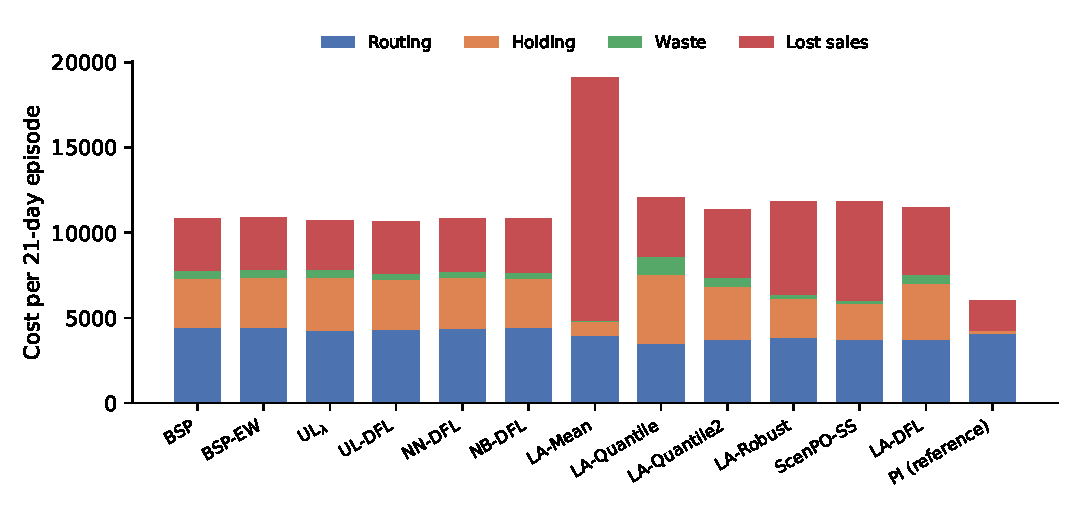
\includegraphics[width=0.85\textwidth]{fig_components.pdf}
\caption{Cost composition of each policy in the base case.}\label{fig:components}
\end{figure}

Four observations stand out. First, uncertainty is expensive: with perfect demand information the same lookahead costs \costPIBase{}, about half of the best implementable policy, almost entirely because lost sales and holding vanish. Second, point forecasts are a poor input for perishable replenishment. LA-Mean plans to sell exactly the expected demand and loses \lostLAMeanBase{} per episode in lost sales (fill rate \fillLAMeanBase\%), as Proposition~\ref{prop:marginal} suggests when $p_u$ is four times $p_s$. Third, among the policies without learning, the three stock-age-based inventory rules are the cheapest: UL$_\lambda$, BSP and BSP-EW cost between \costULBase{} and \costBSPEWBase{} with a fill rate of \fillULBase\% and a waste rate of about 2.5\%. With daily review, little of the current stock is at risk of expiring before it is sold, so the waste correction of BSP-EW rarely changes an order.

Fourth, integration with routing does reduce travel but loses more on the inventory side. The uncertainty-aware lookahead policies visit 7.7--9.0 stores per day instead of 9.2--9.6 and save about 500--1,000 in routing, but LA-Quantile and ScenPO-SS hold 26--37\% more stock than the rules and waste about twice as much (waste rates \wasteScenPOBase\% and \wasteLAQBase\%), while LA-Robust avoids the waste at the price of a fill rate of \fillLARobBase\%. A deterministic plan that covers two or three days with quantile targets stacks a safety buffer on every covered day, even though the next day's re-planning will correct any shortfall. LA-Quantile2, which keeps the 0.9 quantile only for the implemented day and plans later days at the 0.8 quantile, halves the waste rate of LA-Quantile (\wasteLAQTwoBase\% vs.\ \wasteLAQBase\%) and costs 5.7\% less; the scenario model reduces lost sales but, because its single plan must work for all scenarios, it also covers several days generously.

\begin{table}[H]
\centering\footnotesize
\caption{Paired episode-level comparisons of UL-DFL with every other policy (base case, 100 episodes). Negative differences favour UL-DFL. Holm adjustment over the five prespecified primary comparisons of UL-DFL.}\label{tab:testsul}
\setlength{\tabcolsep}{4pt}
\resizebox{\textwidth}{!}{\begin{tabular}{lrrrrrrr}
\toprule
Comparison & Mean diff. & 95\% bootstrap CI & Rel. (\%) & Wins (\%) & $p$ ($t$) & $p$ (Wilcoxon) & Holm $p$ \\
\midrule
UL-DFL $-$ BSP & -213.8 & [-265.8, -160.5] & -2.0 & 80 & $<$0.001 & $<$0.001 & -- \\
UL-DFL $-$ BSP-EW & -236.1 & [-289.0, -182.5] & -2.2 & 80 & $<$0.001 & $<$0.001 & $<$0.001 \\
UL-DFL $-$ UL$_\lambda$ & -107.4 & [-153.1, -60.5] & -1.1 & 67 & $<$0.001 & $<$0.001 & $<$0.001 \\
UL-DFL $-$ NN-DFL & -201.3 & [-254.4, -149.7] & -1.7 & 78 & $<$0.001 & $<$0.001 & -- \\
UL-DFL $-$ NB-DFL & -180.5 & [-225.4, -136.3] & -1.6 & 80 & $<$0.001 & $<$0.001 & -- \\
UL-DFL $-$ LA-Mean & -8,465.5 & [-8,764.1, -8,175.6] & -44.4 & 100 & $<$0.001 & $<$0.001 & -- \\
UL-DFL $-$ LA-Quantile & -1,434.2 & [-1,585.6, -1,278.2] & -11.8 & 98 & $<$0.001 & $<$0.001 & -- \\
UL-DFL $-$ LA-Quantile2 & -752.9 & [-872.7, -629.9] & -6.3 & 92 & $<$0.001 & $<$0.001 & $<$0.001 \\
UL-DFL $-$ LA-Robust & -1,193.9 & [-1,313.2, -1,076.2] & -10.0 & 99 & $<$0.001 & $<$0.001 & -- \\
UL-DFL $-$ ScenPO-SS & -1,199.2 & [-1,342.1, -1,056.2] & -10.3 & 95 & $<$0.001 & $<$0.001 & $<$0.001 \\
UL-DFL $-$ LA-DFL & -819.9 & [-958.9, -684.2] & -6.7 & 95 & $<$0.001 & $<$0.001 & $<$0.001 \\
UL-DFL $-$ PI & 4,630.0 & [4,454.8, 4,800.8] & 87.0 & 0 & $<$0.001 & $<$0.001 & -- \\
\bottomrule
\end{tabular}
}
\end{table}

UL-DFL is the cheapest implementable policy (Table~\ref{tab:testsul}). It costs \ULabsrelULBase\% less than the tuned UL$_\lambda$ from which it starts (95\% CI \ULciULBase{}, lower in \ULwinULBase\% of the episodes), \ULabsrelBSPEWBase\% less than BSP-EW, \ULabsrelScenPOBase\% less than ScenPO-SS, \ULabsrelLAQTwoBase\% less than LA-Quantile2 and \ULabsrelDFLBase\% less than LA-DFL; all five primary comparisons are significant after Holm adjustment ($p<0.001$). The gain over UL$_\lambda$ is a waste reduction: at the same fill rate (\fillULDFLBase\%) and almost the same lost-sales cost, UL-DFL lowers the waste rate from \wasteULBase\% to \wasteULDFLBase\%, i.e.\ it throws away a fifth fewer units, while holding and routing costs rise by at most 0.5\%.

\begin{table}[H]
\centering\footnotesize
\caption{Paired episode-level comparisons of LA-DFL with every other policy (base case, 100 episodes). Negative differences favour LA-DFL. Holm adjustment over the five prespecified primary comparisons of LA-DFL.}\label{tab:tests}
\setlength{\tabcolsep}{4pt}
\resizebox{\textwidth}{!}{\begin{tabular}{lrrrrrrr}
\toprule
Comparison & Mean diff. & 95\% bootstrap CI & Rel. (\%) & Wins (\%) & $p$ ($t$) & $p$ (Wilcoxon) & Holm $p$ \\
\midrule
LA-DFL $-$ BSP & 696.8 & [551.8, 844.2] & 6.4 & 18 & $<$0.001 & $<$0.001 & -- \\
LA-DFL $-$ BSP-EW & 662.5 & [517.0, 810.7] & 6.0 & 21 & $<$0.001 & $<$0.001 & $<$0.001 \\
LA-DFL $-$ UL$_\lambda$ & 749.0 & [606.5, 891.8] & 7.0 & 14 & $<$0.001 & $<$0.001 & $<$0.001 \\
LA-DFL $-$ UL-DFL & 839.7 & [705.7, 972.4] & 7.8 & 6 & $<$0.001 & $<$0.001 & -- \\
LA-DFL $-$ NN-DFL & 677.0 & [556.9, 797.0] & 6.2 & 13 & $<$0.001 & $<$0.001 & -- \\
LA-DFL $-$ LA-Mean & -7,822.9 & [-8,167.1, -7,477.1] & -40.4 & 100 & $<$0.001 & $<$0.001 & -- \\
LA-DFL $-$ LA-Quantile & -573.7 & [-683.7, -465.2] & -4.9 & 84 & $<$0.001 & $<$0.001 & $<$0.001 \\
LA-DFL $-$ LA-Quantile2 & 115.0 & [41.2, 190.6] & 1.0 & 41 & 0.004 & 0.015 & -- \\
LA-DFL $-$ LA-Robust & -400.0 & [-542.4, -255.7] & -3.4 & 70 & $<$0.001 & $<$0.001 & $<$0.001 \\
LA-DFL $-$ ScenPO-SS & -154.5 & [-365.6, 67.9] & -1.6 & 59 & 0.167 & 0.124 & 0.167 \\
LA-DFL $-$ PI & 5,789.9 & [5,575.4, 6,009.5] & 110.2 & 0 & $<$0.001 & $<$0.001 & -- \\
\bottomrule
\end{tabular}
}
\end{table}

LA-DFL improves the deterministic lookahead from which it starts (Table~\ref{tab:tests}). It reduces cost by \absrelLAQBase\% relative to LA-Quantile (95\% CI \ciLAQBase{}, lower in \winLAQBase\% of the episodes) and by \absrelLARobBase\% relative to LA-Robust; it is \absrelScenPOBase\% cheaper than ScenPO-SS, which is not significant (Holm-adjusted $p=$ \pholmScenPOBase{}). It does so by halving the waste rate of LA-Quantile (\wasteDFLBase\% vs.\ \wasteLAQBase\%) while accepting somewhat more lost sales. The simple LA-Quantile2, however, is \absrelLAQTwoBase\% cheaper still (CI \ciLAQTwoBase{}): the gain of LA-DFL over LA-Quantile is captured by a day-specific quantile level, which LA-DFL discovered (Section~\ref{sec:dflresults}) but did not improve on. LA-DFL also remains \absrelBSPEWBase\% more expensive than BSP-EW and \absrelULBase\% more expensive than UL$_\lambda$, both significant.

\subsection{What the decision-focused corrections learn}\label{sec:dflresults}

Table~\ref{tab:ulcorrections} summarises the learned corrections of UL-DFL on the delivery decisions it takes in the 100 base-case test episodes (the rule triggers a delivery on 94\% of the store-days; on the others the correction has no effect). The average correction is nearly zero: the tuned 0.95 level is right on average. What the network learns is \emph{when} to deviate from it, along two dimensions that a one-day order-up-to rule cannot see. On promotion days it lowers the level to an implied service level of about 0.89, i.e.\ by about a third of a day of mean demand. Promotions raise the forecast spread, so the 0.95 quantile lies far above the expected demand, and whatever is left when the promotion ends meets regular demand and ages. Over the week it raises the level from Wednesday to Friday (implied levels 0.96--0.97) and lowers it from Saturday to Monday (0.92--0.93): a unit left over before the weekend is sold in the Saturday peak, whereas a unit left over after it meets lower demand for the rest of its shelf life. The age of the stock on hand matters little, because the rule's order quantity already nets out the stock projected to expire. Both corrections reduce the stock that is still on the shelf when demand falls, which is where the waste of the rule arises.

\begin{table}[H]
\centering\footnotesize
\caption{Learned corrections of UL-DFL on the delivery decisions of 100 test episodes (base case): mean correction $\delta_\theta$ of the order-up-to level in units of the forecast scale, implied service level $\Phi(z_{0.95}+\delta_\theta)$, and change of the order-up-to level in days of mean store demand. Stock is measured in days of mean store demand.}\label{tab:ulcorrections}
\resizebox{0.85\textwidth}{!}{\begin{tabular}{lrrrr}
\toprule
Delivery decisions & $n$ & Correction $\delta_\theta$ (SD) & Implied service level & Change of $S$ (days) \\
\midrule
all delivery decisions & 18,952 & -0.13 (0.30) & 0.940 & -0.07 \\
no promotion & 16,404 & -0.08 (0.27) & 0.947 & -0.03 \\
promotion & 2,548 & -0.48 (0.27) & 0.890 & -0.37 \\
Mon & 2,715 & -0.31 (0.20) & 0.921 & -0.14 \\
Tue & 2,653 & -0.14 (0.22) & 0.941 & -0.07 \\
Wed & 2,745 & +0.01 (0.20) & 0.958 & -0.01 \\
Thu & 2,725 & +0.21 (0.23) & 0.972 & +0.09 \\
Fri & 2,755 & +0.06 (0.23) & 0.961 & +0.02 \\
Sat & 2,854 & -0.39 (0.20) & 0.908 & -0.23 \\
Sun & 2,505 & -0.35 (0.21) & 0.914 & -0.17 \\
stock <0.25 d & 4,450 & -0.09 (0.30) & 0.945 & -0.05 \\
stock 0.25-0.5 d & 2,595 & -0.12 (0.29) & 0.941 & -0.06 \\
stock >0.5 d & 11,907 & -0.15 (0.31) & 0.937 & -0.08 \\
no expiring units & 13,299 & -0.11 (0.30) & 0.942 & -0.06 \\
units expiring today & 5,653 & -0.19 (0.30) & 0.933 & -0.10 \\
\bottomrule
\end{tabular}
}
\end{table}

Table~\ref{tab:corrections} reports the corrections of LA-DFL on the decision states of 20 test episodes. Here the dominant pattern is temporal within the plan. For the implemented day the network keeps the target at about the 0.91 quantile, essentially the tuned LA-Quantile level, but it lowers the targets of the second and third lookahead days to about the 0.80 and 0.77 quantiles. In inventory terms, the network has learned that only today's shortfall is irreversible: tomorrow's planned demand will be re-planned with tomorrow's stock and forecast, so a full safety buffer on that day mostly turns into carried stock and, with a three-day shelf life, into waste. This is precisely the recourse that a deterministic lookahead ignores and that Proposition~\ref{prop:dfl} lets the gradient account for. Context-specific corrections are small: targets are lowered somewhat more on promotion days and slightly less when the store holds more or older stock. The day-specific levels learned by LA-DFL are those that the tuning of LA-Quantile2 selects, $(0.9,0.8)$, which explains why the two policies perform alike.

\begin{table}[H]
\centering\footnotesize
\caption{Learned corrections of LA-DFL on the decision states of 20 test episodes (base case): mean correction $\delta_\theta$ in forecast-scale units, implied quantile level of the planning target, and target relative to the mean forecast. $k$ is the lookahead offset; stock is measured in days of mean store demand.}\label{tab:corrections}
\resizebox{0.85\textwidth}{!}{\begin{tabular}{lrrrr}
\toprule
Targets & $n$ & Correction $\delta_\theta$ (SD) & Implied quantile level & Target / mean forecast \\
\midrule
all & 12,600 & -0.37 (0.38) & 0.826 & 1.46 \\
k=0 & 4,200 & +0.12 (0.15) & 0.910 & 1.67 \\
k=1 & 4,200 & -0.53 (0.15) & 0.804 & 1.38 \\
k=2 & 4,200 & -0.69 (0.17) & 0.765 & 1.31 \\
no promotion & 11,078 & -0.36 (0.39) & 0.828 & 1.45 \\
promotion & 1,522 & -0.47 (0.32) & 0.818 & 1.53 \\
stock <0.25 d & 2,694 & -0.42 (0.39) & 0.816 & 1.43 \\
stock 0.25-0.75 d & 4,059 & -0.40 (0.38) & 0.821 & 1.45 \\
stock >0.75 d & 5,847 & -0.33 (0.38) & 0.835 & 1.48 \\
no expiring units & 8,088 & -0.39 (0.38) & 0.822 & 1.45 \\
units expiring today & 4,512 & -0.33 (0.38) & 0.834 & 1.48 \\
\bottomrule
\end{tabular}
}
\end{table}

For both learners the closed-loop validation cost improved during the first three to five epochs and deteriorated afterwards (Figure~\ref{fig:dfltraining}), which is why model selection on closed-loop validation cost is part of the method. The result does not depend on a lucky seed (Table~\ref{tab:seeds}): the three UL-DFL networks are 0.8--0.9\% cheaper than UL$_\lambda$ on the base-case test set, and the three LA-DFL networks 3.5--4.7\% cheaper than LA-Quantile.

\begin{figure}[H]
\centering
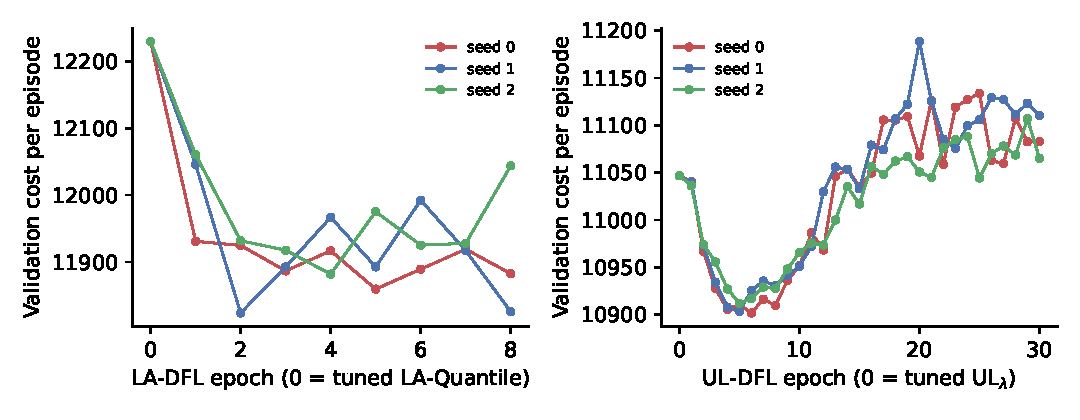
\includegraphics[width=0.9\textwidth]{fig_dfl_training.pdf}
\caption{Closed-loop validation cost by training epoch and seed (base case). Left: LA-DFL, epoch 0 is the tuned LA-Quantile policy. Right: UL-DFL, epoch 0 is the tuned UL$_\lambda$ rule.}\label{fig:dfltraining}
\end{figure}

\begin{table}[H]
\centering\footnotesize
\caption{Test-cost difference (\%) of each trained network relative to the policy it starts from, by seed; ``selected'' is the network chosen on validation cost.}\label{tab:seeds}
\begin{tabular}{llrrrr}
\toprule
Setting & Comparison & Selected (\%) & Seed 0 & Seed 1 & Seed 2 \\
\midrule
Base (fresh test) & UL-DFL vs UL$_\lambda$ & -1.05 & -1.05 & -1.02 & -0.98 \\
Base (fresh test) & NN-DFL vs UL$_\lambda$ & +0.75 & +0.49 & +0.86 & +0.75 \\
Base (fresh test) & NB-DFL vs UL$_\lambda$ & +0.57 & +0.52 & +0.57 & +0.89 \\
Base & UL-DFL vs UL$_\lambda$ & -0.81 & -0.81 & -0.75 & -0.93 \\
Base & NN-DFL vs UL$_\lambda$ & +1.25 & +1.26 & +1.18 & +1.25 \\
Base & NB-DFL vs UL$_\lambda$ & +1.00 & +0.97 & +1.00 & +1.26 \\
Base & LA-DFL vs LA-Quantile & -4.86 & -3.71 & -4.86 & -3.59 \\
Clustered & UL-DFL vs UL$_\lambda$ & -1.21 & -1.21 & -1.17 & -1.15 \\
Clustered & NN-DFL vs UL$_\lambda$ & +0.02 & +0.08 & +0.02 & +0.16 \\
Clustered & NB-DFL vs UL$_\lambda$ & -0.27 & -0.21 & -0.27 & +0.18 \\
Mixed & UL-DFL vs UL$_\lambda$ & -1.02 & -1.02 & -1.02 & -0.95 \\
Mixed & NN-DFL vs UL$_\lambda$ & +0.28 & +0.25 & +0.04 & +0.28 \\
Mixed & NB-DFL vs UL$_\lambda$ & -0.03 & +0.01 & -0.03 & +0.29 \\
$m=2$ & UL-DFL vs UL$_\lambda$ & -1.12 & -1.11 & -1.00 & -1.12 \\
$m=2$ & NN-DFL vs UL$_\lambda$ & -0.49 & -0.61 & -0.55 & -0.49 \\
$m=2$ & NB-DFL vs UL$_\lambda$ & -0.42 & -0.34 & -0.21 & -0.42 \\
$m=4$ & UL-DFL vs UL$_\lambda$ & -0.30 & -0.30 & -0.27 & -0.19 \\
$m=4$ & NN-DFL vs UL$_\lambda$ & +2.49 & +2.40 & +2.47 & +2.42 \\
$m=4$ & NB-DFL vs UL$_\lambda$ & +1.66 & +1.66 & +2.09 & +1.96 \\
$p_u=10$ & UL-DFL vs UL$_\lambda$ & -0.96 & -0.92 & -0.96 & -0.89 \\
$p_u=10$ & NN-DFL vs UL$_\lambda$ & +1.15 & +1.25 & +1.25 & +1.15 \\
$p_u=10$ & NB-DFL vs UL$_\lambda$ & +0.84 & +0.88 & +0.84 & +0.90 \\
$p_u=40$ & UL-DFL vs UL$_\lambda$ & -0.84 & -0.89 & -0.84 & -0.88 \\
$p_u=40$ & NN-DFL vs UL$_\lambda$ & +0.68 & +0.68 & +0.63 & +1.08 \\
$p_u=40$ & NB-DFL vs UL$_\lambda$ & +1.30 & +1.59 & +1.30 & +1.55 \\
$\rho=1.10$ & UL-DFL vs UL$_\lambda$ & -0.81 & -0.81 & -0.76 & -0.76 \\
$\rho=1.10$ & NN-DFL vs UL$_\lambda$ & +0.74 & +0.47 & +0.74 & +0.79 \\
$\rho=1.10$ & NB-DFL vs UL$_\lambda$ & +0.65 & +0.66 & +0.65 & +0.76 \\
$\rho=1.60$ & UL-DFL vs UL$_\lambda$ & -0.30 & -0.31 & -0.30 & -0.35 \\
$\rho=1.60$ & NN-DFL vs UL$_\lambda$ & +1.54 & +1.66 & +1.75 & +1.54 \\
$\rho=1.60$ & NB-DFL vs UL$_\lambda$ & +1.32 & +1.33 & +1.32 & +1.30 \\
High var. & UL-DFL vs UL$_\lambda$ & -0.00 & +0.04 & -0.00 & -0.18 \\
High var. & NN-DFL vs UL$_\lambda$ & +0.86 & +0.74 & +0.92 & +0.86 \\
High var. & NB-DFL vs UL$_\lambda$ & +1.30 & +1.39 & +1.30 & +1.56 \\
$c^{\mathrm{r}}=3$ & UL-DFL vs UL$_\lambda$ & -0.81 & -0.93 & -0.81 & -0.73 \\
$c^{\mathrm{r}}=3$ & NN-DFL vs UL$_\lambda$ & +4.56 & +4.69 & +4.65 & +4.56 \\
$c^{\mathrm{r}}=3$ & NB-DFL vs UL$_\lambda$ & +4.50 & +4.30 & +4.50 & +4.39 \\
30\% LIFO & UL-DFL vs UL$_\lambda$ & -0.80 & -0.80 & -0.75 & -0.82 \\
30\% LIFO & NN-DFL vs UL$_\lambda$ & +1.75 & +1.67 & +2.02 & +1.75 \\
30\% LIFO & NB-DFL vs UL$_\lambda$ & +1.43 & +1.39 & +1.43 & +1.56 \\
30\% LIFO & LA-DFL vs LA-Quantile & -4.94 & -4.43 & -4.94 & -3.43 \\
Real data & UL-DFL vs UL$_\lambda$ & +0.62 & +0.51 & +0.09 & +0.62 \\
Real data & NN-DFL vs UL$_\lambda$ & +1.44 & +1.78 & +1.44 & +1.60 \\
Real data & NB-DFL vs UL$_\lambda$ & +1.13 & +1.13 & +1.37 & +1.70 \\
\bottomrule
\end{tabular}

\end{table}

\subsection{Can re-tuning the rule reproduce UL-DFL?}\label{sec:frontier}

A natural objection is that UL-DFL merely finds better values of the rule's parameters than the tuning grid of Section~\ref{sec:design}. Figure~\ref{fig:frontier} places UL-DFL in the waste--service plane together with 124 parameterisations of the rules, all evaluated on the base-case test episodes: UL$_\lambda$ with $\lambda=1$, ten service levels $\alpha$ between 0.85 and 0.99 and eight trigger levels $\beta$ between 0.5 and 0.99, UL$_\lambda$ with $\lambda\in\{2,3\}$ on the original grid, and daily BSP and BSP-EW at the same ten service levels. No parameterisation serves at least UL-DFL's fill rate (96.2\%) with no more waste: at that fill rate the least waste any rule achieves is 2.48\% of the delivered units, against 1.98\% for UL-DFL. The learned corrections move the policy beyond the waste--service frontier of the rules, which no choice of a single service level and trigger can do.

In total cost the comparison is closer. The cheapest of the 124 rules in hindsight---selected on the test episodes themselves, an advantage UL-DFL does not have---is UL$_\lambda$ with $\alpha=0.96$ and $\beta=0.8$. It costs 10,715 per episode, the same as UL-DFL (difference $-0.05\%$, 95\% CI $[-59, 46]$), but it gets there differently: its lower trigger saves routing (4,168 vs.\ 4,337), and it wastes 2.80\% of the delivered units, 41\% more than UL-DFL. Part of the 0.8\% cost advantage of UL-DFL over the tuned rule therefore reflects the resolution of the tuning grid; the waste reduction at a given service level does not. The real-data case gives the same picture: no rule parameterisation reaches UL-DFL's fill rate (93.8\%) with its waste rate (2.96\%; the least any rule achieves at that fill rate is 3.15\%), and the best rule in hindsight ($\alpha=0.96$, $\beta=0.85$) matches its cost ($+0.02\%$ for UL-DFL, 95\% CI $[-50, 78]$) while wasting 23\% more.

\begin{figure}[H]
\centering
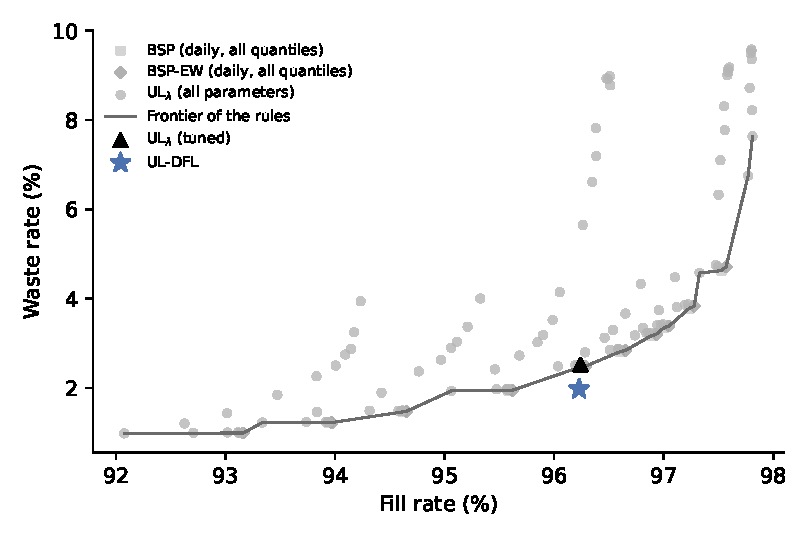
\includegraphics[width=0.62\textwidth]{fig_frontier.pdf}
\caption{Waste rate against fill rate of 124 parameterisations of the rules and of UL-DFL (base case, 100 test episodes). The line connects the rule parameterisations that are not dominated in both measures.}\label{fig:frontier}
\end{figure}

\subsection{Does the learner need the rule?}\label{sec:nndfl}

The converse question is whether the rule contributes anything once a network is trained on realised cost. NN-DFL answers it: it has the same inputs, differentiable simulation, loss, seeds and model selection as UL-DFL, but outputs the delivery directly, without the visit trigger and order-up-to structure of UL$_\lambda$. In the base case it costs \costNNDFLBase{} per episode, \ULabsrelNNDFLBase\% more than UL-DFL (95\% CI of UL-DFL minus NN-DFL \ULciNNDFLBase{}) and more than the tuned UL$_\lambda$ it would replace. It does learn to waste little (waste rate \wasteNNDFLBase\%), but it loses more sales and, lacking a trigger, visits slightly more stores (\visitsNNDFLBase{} per day against \visitsULDFLBase{}). Across the thirteen configurations UL-DFL is significantly cheaper than NN-DFL in twelve, by 0.8--4.9\% (Table~\ref{tab:uldfldiffs}). The gap is largest with expensive routing, where the trigger of UL-DFL cuts store visits to \visitsULDFLRouteThree{} per day while NN-DFL keeps visiting \visitsNNDFLRouteThree{}, and the two tie with a two-day shelf life, where frequent small deliveries suit the short shelf life. NN-DFL is more expensive than UL$_\lambda$ itself in eleven of the thirteen configurations (Table~\ref{tab:seeds}). These comparisons are secondary, because the ablation was added after the primary hypotheses were fixed, but they are consistent: with the same network and learning signal, the gain comes from placing the learner on the rule.

\subsection{Sensitivity analysis}\label{sec:sensitivity}

Table~\ref{tab:sensitivity} reports test costs across the configurations, and Tables~\ref{tab:uldfldiffs} and~\ref{tab:dfldiffs} the paired differences of the two learned policies. \SensitivityText

\begin{table}[H]
\centering\footnotesize
\caption{Mean test cost per episode by configuration (one factor changed at a time; bold: lowest implementable policy), and fill rates of selected policies.}\label{tab:sensitivity}
\setlength{\tabcolsep}{4pt}
\resizebox{\textwidth}{!}{\begin{tabular}{lrrrrrrrrrrrrr}
\toprule
Policy & Base & Clustered & Mixed & $m=2$ & $m=4$ & $p_u=10$ & $p_u=40$ & $\rho=1.10$ & $\rho=1.60$ & High var. & $c^{\mathrm{r}}=3$ & 30\% LIFO & Real data \\
\midrule
BSP & 10,851 & 8,266 & 10,206 & 12,607 & 10,490 & 9,056 & 13,480 & 12,221 & 9,868 & 15,011 & 19,633 & 11,208 & 13,068 \\
BSP-EW & 10,885 & 8,289 & 10,235 & 12,633 & 10,490 & 9,082 & 13,496 & 12,227 & 9,922 & 15,089 & 19,704 & 11,256 & 13,090 \\
UL$_\lambda$ & 10,799 & 8,274 & 10,199 & 12,599 & 10,339 & 8,956 & 13,374 & 12,152 & 9,798 & 14,885 & 18,856 & 11,141 & 13,027 \\
UL-DFL & \textbf{10,708} & \textbf{8,168} & \textbf{10,090} & 12,487 & \textbf{10,324} & \textbf{8,867} & \textbf{13,251} & \textbf{12,063} & \textbf{9,755} & \textbf{14,845} & 18,700 & \textbf{11,057} & \textbf{12,951} \\
NN-DFL & 10,871 & 8,263 & 10,221 & \textbf{12,483} & 10,534 & 9,052 & 13,396 & 12,179 & 9,892 & 14,974 & 19,645 & 11,253 & 13,093 \\
LA-Mean & 19,371 & 17,051 & 18,362 & 19,769 & 19,350 & 12,074 & 33,960 & 19,362 & 19,407 & 25,609 & 24,289 & 19,400 & 21,030 \\
LA-Quantile & 12,122 & 9,735 & 11,520 & 13,954 & 11,289 & 9,314 & 15,490 & 13,327 & 10,405 & 16,398 & 19,157 & 12,574 & 14,478 \\
LA-Quantile2 & 11,433 & 9,110 & 10,830 & 13,553 & 10,977 & 9,136 & 15,436 & 13,047 & 10,071 & 15,631 & 18,630 & 11,787 & 14,185 \\
LA-Robust & 11,948 & 9,545 & 11,209 & 13,622 & 11,221 & 9,173 & 15,295 & 13,291 & 10,184 & 15,851 & 18,983 & 12,110 & 14,560 \\
ScenPO-SS & 11,702 & 9,544 & 11,315 & 13,179 & 11,051 & 9,393 & 14,501 & 12,512 & 10,997 & 16,218 & \textbf{18,197} & 12,162 & 13,776 \\
LA-DFL & 11,548 & 9,294 & 11,089 & 14,295 & 11,015 & 9,258 & 15,498 & 13,260 & 10,146 & 16,101 & 19,058 & 11,974 & 14,333 \\
\midrule
PI (reference) & 5,758 & 3,352 & 5,180 & 6,121 & 5,752 & 5,005 & 7,260 & 7,678 & 4,728 & 7,097 & 13,589 & 5,758 & 7,329 \\
\midrule
Fill rate (\%), UL-DFL & 96.2 & 96.2 & 96.2 & 94.8 & 96.6 & 94.6 & 97.1 & 94.8 & 97.1 & 93.1 & 95.9 & 96.2 & 93.8 \\
Fill rate (\%), LA-DFL & 95.1 & 95.2 & 95.1 & 93.1 & 95.4 & 93.4 & 95.8 & 92.8 & 96.3 & 91.9 & 94.9 & 94.9 & 92.1 \\
Fill rate (\%), ScenPO-SS & 95.6 & 96.1 & 95.7 & 95.0 & 95.7 & 92.0 & 97.1 & 93.8 & 96.0 & 92.0 & 94.2 & 95.5 & 93.1 \\
Fill rate (\%), LA-Quantile & 95.7 & 96.2 & 96.1 & 91.2 & 95.9 & 92.7 & 95.8 & 91.6 & 96.3 & 89.1 & 93.0 & 95.6 & 92.8 \\
Fill rate (\%), BSP-EW & 96.3 & 96.3 & 96.3 & 94.5 & 96.3 & 94.7 & 97.0 & 94.5 & 97.4 & 93.8 & 96.3 & 96.2 & 93.8 \\
\bottomrule
\end{tabular}
}
\end{table}

\begin{table}[H]
\centering\footnotesize
\caption{Paired cost difference of UL-DFL relative to each comparator, in percent of the comparator's cost, by configuration. Bold: 95\% paired bootstrap interval excludes zero.}\label{tab:uldfldiffs}
\resizebox{\textwidth}{!}{\begin{tabular}{lrrrrrrrrrrrrr}
\toprule
UL-DFL & Base & Clustered & Mixed & $m=2$ & $m=4$ & $p_u=10$ & $p_u=40$ & $\rho=1.10$ & $\rho=1.60$ & High var. & $c^{\mathrm{r}}=3$ & 30\% LIFO & Real data \\
\midrule
vs UL$_\lambda$ & \textbf{-0.8} & \textbf{-1.2} & \textbf{-1.0} & \textbf{-1.1} & -0.3 & \textbf{-1.0} & \textbf{-0.8} & \textbf{-0.8} & -0.3 & -0.0 & \textbf{-0.8} & \textbf{-0.8} & \textbf{+0.6} \\
vs BSP-EW & \textbf{-2.2} & \textbf{-1.5} & \textbf{-1.4} & \textbf{-1.8} & \textbf{-2.2} & \textbf{-2.4} & \textbf{-2.2} & \textbf{-1.9} & \textbf{-2.1} & \textbf{-1.8} & \textbf{-5.4} & \textbf{-2.6} & -0.5 \\
vs ScenPO-SS & \textbf{-10.8} & \textbf{-15.9} & \textbf{-13.6} & \textbf{-4.4} & \textbf{-13.4} & \textbf{-9.9} & \textbf{-13.2} & \textbf{-4.7} & \textbf{-19.6} & \textbf{-11.5} & \textbf{-3.4} & \textbf{-9.9} & \textbf{-8.3} \\
vs LA-DFL & \textbf{-7.5} & \textbf{-11.4} & \textbf{-8.5} & \textbf{-12.3} & \textbf{-6.7} & \textbf{-4.1} & \textbf{-14.6} & \textbf{-9.4} & \textbf{-4.1} & \textbf{-7.8} & \textbf{-2.1} & \textbf{-7.9} & \textbf{-9.6} \\
vs LA-Quantile2 & \textbf{-6.6} & \textbf{-9.8} & \textbf{-6.1} & \textbf{-7.6} & \textbf{-6.5} & \textbf{-2.9} & \textbf{-14.3} & \textbf{-7.8} & \textbf{-3.4} & \textbf{-5.0} & +0.1 & \textbf{-6.6} & \textbf{-8.4} \\
vs NN-DFL & \textbf{-2.0} & \textbf{-1.1} & \textbf{-1.2} & \textbf{-0.6} & \textbf{-2.7} & \textbf{-2.1} & \textbf{-1.4} & \textbf{-1.5} & \textbf{-1.8} & \textbf{-0.8} & \textbf{-5.1} & \textbf{-2.4} & -0.8 \\
\bottomrule
\end{tabular}
}
\end{table}

\begin{table}[H]
\centering\footnotesize
\caption{Paired cost difference of LA-DFL relative to each comparator, in percent of the comparator's cost, by configuration. Bold: 95\% paired bootstrap interval excludes zero.}\label{tab:dfldiffs}
\resizebox{\textwidth}{!}{\begin{tabular}{lrrrrrrrrrrrrr}
\toprule
LA-DFL & Base & Clustered & Mixed & $m=2$ & $m=4$ & $p_u=10$ & $p_u=40$ & $\rho=1.10$ & $\rho=1.60$ & High var. & $c^{\mathrm{r}}=3$ & 30\% LIFO & Real data \\
\midrule
vs LA-Quantile & \textbf{-4.9} & \textbf{-5.0} & \textbf{-3.9} & \textbf{+2.1} & \textbf{-2.5} & -0.7 & +0.0 & -0.8 & \textbf{-2.4} & \textbf{-1.7} & -0.4 & \textbf{-4.9} & -1.4 \\
vs LA-Quantile2 & \textbf{+1.0} & \textbf{+1.9} & \textbf{+2.8} & \textbf{+5.7} & +0.3 & \textbf{+1.4} & +0.7 & \textbf{+1.8} & +0.8 & \textbf{+3.3} & \textbf{+2.4} & \textbf{+1.5} & +1.5 \\
vs ScenPO-SS & -1.6 & -3.4 & \textbf{-2.4} & \textbf{+7.7} & -0.5 & \textbf{-1.4} & \textbf{+6.4} & \textbf{+5.6} & \textbf{-7.6} & -0.8 & \textbf{+4.8} & -1.9 & \textbf{+4.5} \\
vs LA-Robust & \textbf{-3.4} & \textbf{-2.9} & -1.1 & \textbf{+4.8} & \textbf{-1.8} & \textbf{+0.9} & +1.9 & -0.2 & -0.3 & \textbf{+1.8} & +0.5 & -1.2 & -0.6 \\
vs BSP-EW & \textbf{+6.0} & \textbf{+11.8} & \textbf{+8.1} & \textbf{+12.7} & \textbf{+5.1} & \textbf{+1.9} & \textbf{+15.2} & \textbf{+8.6} & \textbf{+2.2} & \textbf{+6.8} & \textbf{-3.3} & \textbf{+6.2} & \textbf{+10.5} \\
vs UL$_\lambda$ & \textbf{+7.0} & \textbf{+12.1} & \textbf{+8.6} & \textbf{+13.1} & \textbf{+6.6} & \textbf{+3.5} & \textbf{+16.0} & \textbf{+9.2} & \textbf{+3.5} & \textbf{+8.4} & \textbf{+1.3} & \textbf{+7.4} & \textbf{+11.2} \\
\bottomrule
\end{tabular}
}
\end{table}

\begin{figure}[H]
\centering
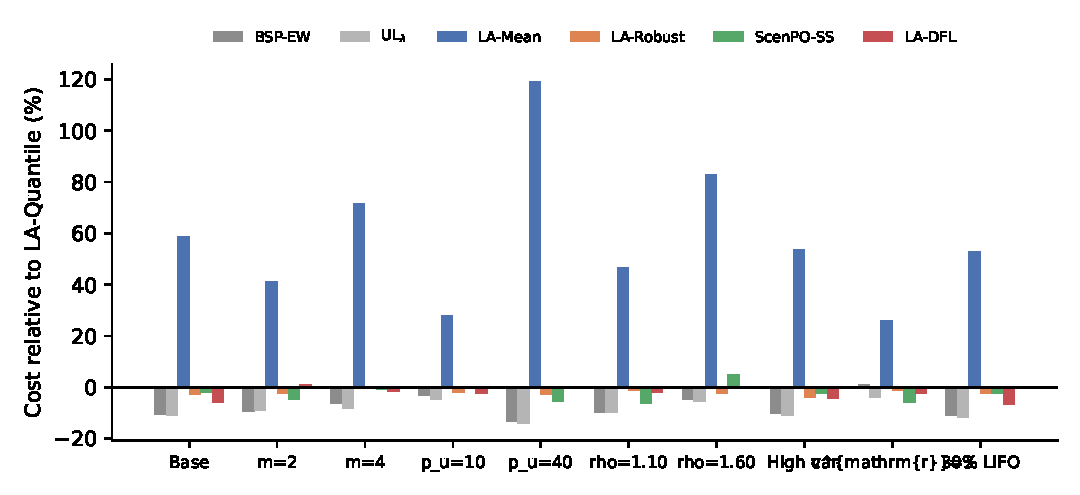
\includegraphics[width=0.95\textwidth]{fig_sensitivity.pdf}
\caption{Cost of selected policies relative to LA-Quantile, by configuration (LA-Mean is omitted for readability).}\label{fig:sensitivity}
\end{figure}

\subsection{Real-data case}\label{sec:realresults}

On observed demand (column ``Real data'' of Tables~\ref{tab:sensitivity} and~\ref{tab:uldfldiffs}) the ranking of the policy families is the same as in the synthetic base case. UL-DFL is the cheapest policy (\costULDFLFresh{} per episode), \ULabsrelULFresh\% below UL$_\lambda$ (95\% CI \ULciULFresh{}, Holm-adjusted $p=\ULpholmULFresh$), \ULabsrelBSPEWFresh\% below BSP-EW and \ULabsrelScenPOFresh\% below ScenPO-SS, the best integrated policy. Without learning, the rules (\costULFresh--\costBSPEWFresh) are again cheaper than every integrated policy, and LA-Mean is again the most expensive. Service is lower than in the synthetic study for all policies (fill rate \fillULFresh\% for UL$_\lambda$), because observed demand is more volatile and its promotion and weekend peaks occasionally exceed the daily fleet capacity.

The saving of UL-DFL has a different composition on real data. It reduces lost sales by 2.3\% and waste by 4.6\% while holding 3.1\% more stock, and its fill rate rises from \fillULFresh\% to \fillULDFLFresh\%. The learned corrections explain why. Demand in these data peaks at the weekend (Saturday and Sunday are 16\% and 29\% above the average day of the history window, Wednesday to Friday 8--10\% below it), and the network raises the order-up-to level on Thursday and Friday (implied service levels 0.96 and 0.99, Friday by 0.3 days of mean demand) and lowers it on Saturday to Monday (0.92, 0.85 and 0.92). Units delivered on Friday are carried into the weekend peak, which a one-day level misses, and units left over on Sunday meet the weaker start of the week. This is the same rule as in the synthetic data---build stock before the weekly peak, cut it on the days after---but here the peak is larger and falls on different days, so the correction mostly prevents weekend stock-outs instead of removing waste. Discounts, which are offered on 44\% of the store-days in these data and are mostly small, have no systematic effect on the correction. LA-DFL is \absrelLAQFresh\% cheaper than LA-Quantile, which is not significant (Holm-adjusted $p=\pholmLAQFresh$), and LA-Quantile2 is again cheaper than LA-DFL, though not significantly.

\subsection{Store-level service}\label{sec:stores}

Average fill rates hide how service is distributed over the network (Figure~\ref{fig:stores}). In all three layouts the inventory rules, with or without learning, serve every store at least 95.4\%. The deterministic lookahead policies do not: in the base layout their worst-served store, one of the more distant stores, reaches only 89.9--90.6\% (LA-Quantile, LA-Quantile2, LA-Robust, LA-DFL), and in the clustered and mixed layouts 89.6--94.5\%. Consolidating deliveries saves the most travel at stores that are expensive to reach, and the plan then accepts shortages there; in the base layout the store fill rate of the lookahead policies falls with distance from the depot (correlation $-0.24$ to $-0.26$ for LA-Quantile, LA-Quantile2 and LA-DFL), whereas that of the rules rises with it ($+0.81$). In the clustered and mixed layouts, where most stores are about equally far from the depot, the link with distance is weaker but the gap in the worst-served store remains. ScenPO-SS spreads service more evenly (worst store at least 95.0\% in all three layouts). This effect is relevant for retailers with service-level agreements per store: an integrated plan may concentrate stock-outs at individual stores even when its average fill rate is high.

\begin{figure}[H]
\centering
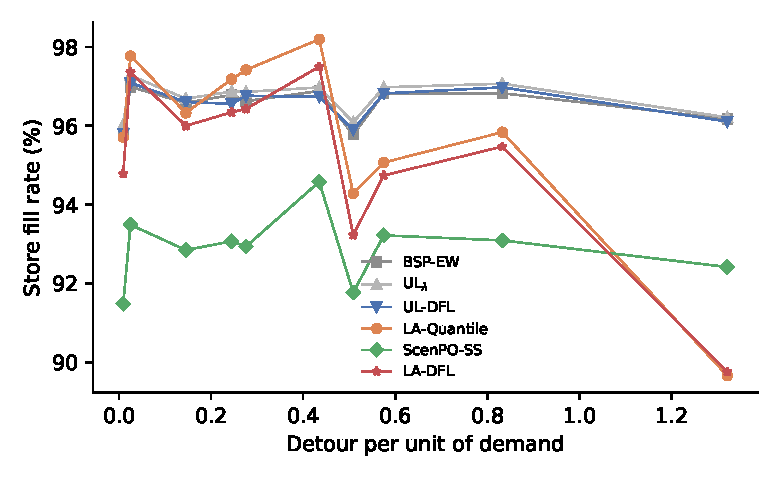
\includegraphics[width=0.6\textwidth]{fig_store_service.pdf}
\caption{Store fill rate against distance from the depot (base case, mean over 100 test episodes).}\label{fig:stores}
\end{figure}

\subsection{Computation}\label{sec:computation}

All \ndecisionsBase{} lookahead decisions of the base-case test were solved to a proven gap of at most \maxgapBase\%, with \nonoptBase{} time-limit stops and \fallbacksBase{} fallbacks; the same holds in every configuration reported. With 15 decisions solved in parallel, a deterministic lookahead decision takes about \secsLAQBase{} seconds and a ScenPO-SS decision \secsScenPOBase{} seconds; the rules, with or without learned corrections, need milliseconds. Training one UL-DFL network (30 epochs over 200 episodes, including closed-loop validation after every epoch) took about two minutes; training one LA-DFL network (2,100 states, eight epochs including MILP re-solves and closed-loop validation) about 45 minutes. The complete base case, including tuning of all policies and three seeds of each learner, took 4.2 hours, and each other configuration 1.0--2.6 hours with 13--15 parallel workers (training three NN-DFL networks adds about ten minutes).

The lookahead policies are deterministic: solving the same decision twice returns the same plan. Their closed-loop cost is nevertheless sensitive to negligible changes in the planning input, because several plans lie within the 0.5\% optimality gap and the solver returns the first one it proves; a different plan on one day changes the stock and therefore every later decision. To quantify this noise floor we re-ran LA-Quantile on the test episodes with its planning targets rounded to single precision, a relative change below $10^{-7}$. The plan changed on at least one day in each of the \noiseN{} test episodes of the thirteen configurations, and episode costs moved by \noiseSDBase\% (standard deviation) in the base case, between \noiseMinBase\% and \noiseMaxBase\%, and by \noiseSDLo--\noiseSDHi\% across configurations. Averaged over 100 episodes these changes largely cancel (mean change at most \noiseAbsMeanMax\% in absolute value, standard error at most \noiseSEHi\%). Paired comparisons remain valid, because this variation is part of the episode-level noise they account for, but differences of well below one percent between two lookahead policies should not be interpreted as a systematic effect. The rule-based policies, including UL-DFL, do not solve an optimisation model for their orders and are not affected.

\subsection{Verification of the structural results}\label{sec:verification}

Table~\ref{tab:verification} reports numerical checks of the results in Section~\ref{sec:theory} (script \texttt{verify\_theory.py} in the replication package). Theorem~\ref{thm:fifo}(ii) is checked by solving the recourse a second time with FIFO issuing and greedy service imposed through binary indicator constraints: if the theorem were false, the constrained value would exceed $V_{\mathrm{LP}}$ in some instance. The bound of Proposition~\ref{prop:marginal}(b) is attained in 71\% of the random instances, so it cannot be tightened in general. The physical FIFO cost equals $V_{\mathrm{LP}}$ in 63\% of the random instances; the remaining gap is the value of discarding stock early, which a store does not do in practice.

\begin{table}[H]
\centering\small
\caption{Numerical verification of the structural results.}\label{tab:verification}
\begin{tabular}{p{3.2cm}p{6.6cm}p{4.0cm}}
\toprule
Result & Check & Outcome \\
\midrule
Theorem~\ref{thm:fifo}(i) & 60 lookahead MILPs ($m\in\{2,3,4\}$, 1 or 5 scenarios) with demand from zero to four times fleet capacity & all feasible, all solved to proven gap \\
Theorem~\ref{thm:fifo}(ii) & 3,000 random recourse instances ($m\in\{2,3,4\}$, $H\in\{2,\dots,5\}$, random costs); FIFO- and greedy-constrained MILP value vs.\ $V_{\mathrm{LP}}$ & max.\ absolute difference $10^{-6}$ \\
Theorem~\ref{thm:fifo}(iii) & $V_{\mathrm{LP}}\le C_{\mathrm{FIFO}}$ in the same instances & holds in 3,000/3,000; equality in 63\% \\
Proposition~\ref{prop:marginal}(a) & dual bounds $[-p_u,p_s]$; subgradient inequality in 9,000 random directions & 3,000/3,000; 9,000/9,000 \\
Proposition~\ref{prop:marginal}(b) & autograd derivative of $C_{\mathrm{FIFO}}$ within \eqref{eq:marg} & 3,000/3,000; bound attained in 71\% \\
Proposition~\ref{prop:dfl}(c) & $m=1$, negative-binomial demand (mean 15), SGD on the decision-focused loss (with $m=1$ both learners deliver the learned quantity, so the check covers (a) and (b)) & learned target 20.03; empirical 0.8-quantile 20.0; $F(\tilde d)=0.809$ vs.\ $p_u/(p_u+p_s)=0.8$ \\
Coverage layer & 40 lookahead MILPs; deliveries implied by the visit pattern vs.\ MILP deliveries & 98.7\% of delivered volume reproduced (mean relative $L_1$ deviation 1.3\%) \\
\bottomrule
\end{tabular}
\end{table}


% ============================================================================
\section{Discussion and conclusion}\label{sec:conclusion}
% ============================================================================

\subsection{Managerial implications}

The study asked how contextual forecasts should be turned into replenishment decisions when perishable stock ages and deliveries share vehicles. Five implications follow for planners of fresh-food distribution.

\begin{enumerate}[leftmargin=*]
\item \textbf{Start from a stock-age-based replenishment rule, tune it finely, and benchmark against it before integrating.} Daily replenishment at a high service quantile, with the orders routed optimally, was cheaper than every integrated inventory-routing policy in all settings but the one with expensive routing, by 2.0--11.9\%, across three network layouts, shelf lives of two to four days, lower and higher lost-sales penalties, tighter and looser fleets, more variable demand, partial LIFO issuing and observed demand of a fresh-food retailer; the margin was smallest when lost sales were cheap, so that high service is worth less. In these settings the travel saved by consolidating deliveries is smaller than the extra holding, waste and lost sales that consolidation causes. A finer grid for the service level and the visit trigger alone lowered the cost of the deliver-up-to-level rule by up to 0.6\%. This extends the finding of \citet{haijema2019improved} and \citet{crama2018stochastic} that well-tuned simple rules are hard to beat to a setting with shared routes and contextual forecasts.
\item \textbf{Learn the order-up-to level, not only the forecast, but check that what is learned carries over.} Training the order-up-to level of the deliver-up-to-level rule on the realised cost of its decisions reduced cost by about 1\% in nine of thirteen settings and on fresh test episodes of the base case, where it reached almost the same fill rate with 28\% less waste, which no re-tuning of the rule's service level and trigger achieves. The gain was smallest, and not significant, where the rule already wasted little (four-day shelf life), with a loose fleet, and where demand was too variable for the context to anticipate it. On observed demand of new products the learned corrections did not carry over, and the rule was cheaper: corrections should be validated on products and periods like those on which they will be used, and the rule kept where they are not. The learning also needs the rule: the same network trained to order directly was more expensive than UL-DFL in twelve settings. The policy is operated exactly like the rule: it remains a rule with a visit trigger and an order-up-to level that planners can inspect. The learned corrections translate into practice that does not require machine learning: shift safety stock from the days after the weekly peak to the days before it, and, where promotions widen the forecast spread, lower the order-up-to level on promotion days.
\item \textbf{Integration pays when routing is expensive, and then the safety stock of the plan matters most.} With three times higher travel cost, a lookahead with day-specific quantile levels was the cheapest policy, level with UL-DFL, and every uncertainty-aware lookahead beat daily base-stock. Scenario-based lookahead with the scenario set of \citet{jia2025scenario}, which does not extend beyond the 0.9 quantile of the forecasts, under-stocked; with scenarios drawn from bands of the full quantile grid, which reach further into the upper tail, it would have been the cheapest policy in that setting. Deterministic lookahead with mean forecasts was the worst policy in every setting.
\item \textbf{If a deterministic plan is used, its safety stock should depend on the planning day.} Decision-focused learning on top of the lookahead learned to keep a high service quantile only for the day that is actually executed and to plan later days near the 0.8 quantile. A lookahead with these two quantile levels, tuned on validation data, removes about half of the waste of the single-quantile plan in the base case and was at least as cheap as the learned targets in all thirteen settings.
\item \textbf{Look at store-level service, not only at averages.} Integrated deterministic plans concentrated stock-outs at the store whose visit costs the most travel per unit sold, whereas the inventory rules served all stores alike. Retailers with per-store service targets should constrain or monitor this effect.
\end{enumerate}

\subsection{Limitations and further research}

The synthetic demand is generated by a documented contextual model; the real-data case uses observed sales of one retailer, from which latent demand had to be reconstructed under stock-outs and rescaled to the network's capacities, and from which products whose level shifted strongly were excluded. The test episodes of the synthetic configurations had been evaluated in an earlier round of the study; the primary hypotheses are therefore tested on fresh test episodes of the base case, and the other synthetic configurations are secondary evidence. In the real-data case, model selection on validation episodes did not protect against corrections that failed to transfer to new products; regularising the corrections towards the rule, or validating across products and periods, are natural remedies. Exact routing by enumeration limits the network to about a dozen stores; larger networks require heuristic routing, which would weaken the clean separation between replenishment and routing quality used here. Lead time is zero and each store sells one product; positive lead times would increase the value of stock-age information \citep{broekmeulen2009heuristic}, and multiple products would couple stores through shared vehicle space. The lookahead policies relax routing integrality beyond the implemented day, which favours visiting stores more often than a fully integer lookahead would. ScenPO-SS was implemented with the scenario set of the original study; its cost depends on how far the scenarios reach into the upper tail of the forecast, and tuning this choice on validation data, as done for the quantile levels of the deterministic lookahead, could make it more competitive. UL-DFL learns the order-up-to level but keeps the rule's visit trigger and sees fleet capacity only as a proportional scaling during training; learning the trigger as well, or training against the exact routing cost, could extend its advantage to settings with expensive routing. LA-DFL was trained on the decision states visited by LA-Quantile in one round; iterating between training and data collection, or training the scenario generator of ScenPO-SS decision-focusedly, are natural extensions. Finally, deep reinforcement learning has shown promise for single-location perishable inventory \citep{demoor2022reward,temizoz2025deep}; extending it to the routing-coupled action space studied here is an open problem.

\subsection{Conclusion}

Replenishing perishables on shared routes is a perishable inventory problem first and a routing problem second. Under a common closed-loop simulator with exact optimisation, stock-age-based replenishment rules were the strongest policies without learning unless travel was expensive, in which case a lookahead with day-specific safety quantiles matched them. Decision-focused learning made a well-tuned rule about 1\% cheaper and markedly less wasteful in most settings, including fresh test episodes, by learning from realised cost when to deviate from a fixed service quantile; on observed demand of new products its corrections did not carry over. On top of a deterministic lookahead it revealed why such plans mis-stock, a lesson that a day-specific quantile level implements without learning. The structural results, the experimental protocol and the code are available for testing further policies on the same benchmark.


\section*{Data and code availability}
All code, configuration files, random seeds and result files needed to reproduce every table and figure are provided in the replication package (\texttt{pirp/}, \texttt{experiments/}, \texttt{results/}). The demand data are generated by the package; no proprietary data are used.

\bibliographystyle{elsarticle-harv}
\bibliography{references}

% ============================================================================
\appendix
\section{Proofs}\label{app:proofs}
% ============================================================================

\begin{proof}[Proof of Proposition~\ref{prop:exact}]
Fix $v$ and $k$ and let $R^\star=\{i:z_{ivk}=1\}$. Constraint \eqref{eq:route} gives $\sum_R y_{Rvk}=1$ and $\sum_{R\ni i}y_{Rvk}=z_{ivk}$. For $i\in R^\star$ the second equality equals the first, so every $R$ with $y_{Rvk}>0$ contains $i$; for $i\notin R^\star$ the sum is zero, so no such $R$ contains $i$. Hence $y_{Rvk}>0$ implies $R=R^\star$, and $y_{R^\star vk}=1$. The routing cost is $\mathrm{TSP}(R^\star)$, vehicle loads are at most $Q$ by \eqref{eq:load}, and each store is on at most one vehicle. Every feasible lookahead plan (stores per vehicle, loads, inventory flows) has exactly one representation of this form, which proves exactness.
\end{proof}

\begin{proof}[Proof of Theorem~\ref{thm:fifo}]
(i) Setting $z=0$, $y_{\emptyset vk}=1$, $q=0$, $\zeta=0$ and serving demand from available stock in any order is feasible: day-0 stock satisfies the shelf constraint by assumption and stock only decreases afterwards. All cost terms (travel, holding of carried units, waste, lost sales) are non-negative, so the objective is bounded below by zero; with finitely many assignments and a bounded linear programme for each, an optimum exists.

(ii) Take an optimal recourse solution and view inventory as fungible flows of units per cohort. \emph{Greedy service.} If on day $k$ demand is lost while $\varepsilon>0$ units are left on the shelf, sell $\varepsilon$ of them. Those units originally had one of four fates: sold on a later day (that later sale is now lost; the cost change is $-p_u\varepsilon+p_u\varepsilon-h\varepsilon\cdot(\text{nights saved})\le0$), expired or disposed (saving $p_s\varepsilon$ and holding), or carried beyond the horizon (saving holding). The cost does not increase. \emph{FIFO.} If on day $k$ a younger cohort $r'$ is sold while $\varepsilon$ units of an older cohort $r<r'$ are left, sell $\varepsilon$ older units instead and keep $\varepsilon$ younger ones. The kept younger units replicate the original path of the older units: they are sellable on every day the older units were (their remaining life is longer); where the older units expired at the end of day $k+r-1$, the younger units are disposed on that day at the same cost $p_s$ and with the same number of holding nights; disposal and carrying beyond the horizon are replicated identically. The number of units carried each night is unchanged, so the cost is unchanged. Each exchange reduces $\sum_k\sum_r r\,w_{irk}$ and the feasible set is a polytope, so a finite sequence of exchanges yields an optimal solution with FIFO issuing and greedy service.

(iii) $q$ enters the recourse LP only through the right-hand side of $S_{imk}=q_k$, so $V_{\mathrm{LP}}$ is the value function of an LP in its right-hand side, which is convex and piecewise linear. The physical FIFO trajectory with $\zeta=0$ is feasible for the recourse LP and has cost $C_{\mathrm{FIFO}}$; hence $V_{\mathrm{LP}}\le C_{\mathrm{FIFO}}$. By (ii) there is an optimal solution with FIFO issuing and greedy service; if it uses no disposal it coincides with the physical trajectory and the two values are equal.
\end{proof}

\begin{proof}[Proof of Proposition~\ref{prop:marginal}]
(a) By LP duality, the optimal dual of the constraint $S_{imk}=q_k$ is a subgradient of the value function with respect to $q_k$. Adding $\varepsilon$ to $q_k$ and disposing of these units immediately is feasible and costs $p_s\varepsilon$ (holding $h\varepsilon$ through $S_{imk}$ plus $(p_s-h)\varepsilon$ through $\zeta$), so $V_{\mathrm{LP}}(q+\varepsilon e_k)\le V_{\mathrm{LP}}(q)+p_s\varepsilon$ and $\pi_k\le p_s$. Removing $\varepsilon\le q_k$ units turns at most $\varepsilon$ sales into lost sales and cannot increase holding or waste, so $V_{\mathrm{LP}}(q-\varepsilon e_k)\le V_{\mathrm{LP}}(q)+p_u\varepsilon$ and $\pi_k\ge -p_u$.

(b) $C_{\mathrm{FIFO}}$ is a composition of finitely many $\min$, $\max$ and affine maps of $q$, hence piecewise linear and Lipschitz. Compare the FIFO trajectories with deliveries $q$ and $q+\varepsilon e_k$. On day $k$ the extra units are the freshest and are sold last, so sales of older stock are unchanged. On later days the extra units are older than subsequent deliveries and may displace them, but stock that was older than the extra units is never affected. Therefore, relative to the original trajectory, lost sales can only fall, waste and carried stock can only rise, and the total extra stock $E_\ell$ carried on night $\ell$ satisfies $0\le E_\ell\le\varepsilon$. Each extra unit leaves the system by preventing a lost sale ($-p_u$), by expiring on some day $\tau\le H-1$ ($+p_s$ after at most $\tau-k\le H-1-k$ nights), or by remaining at the end ($H-k$ nights). The cost change per unit is therefore at least $-p_u$ and at most $\max\{p_s+(H-1-k)h,\,(H-k)h\}=p_s+(H-1-k)h$ when $h\le p_s$. Dividing by $\varepsilon$ gives \eqref{eq:marg} for both one-sided derivatives.
\end{proof}

\begin{proof}[Proof of Proposition~\ref{prop:dfl}]
(a) With the visit pattern fixed and no capacity binding, the coverage map gives $q_k=\sum_{j\in W_k}\tilde d_j-U_k(\tilde d)$, where $U_k$ is the planned usable stock that serves the window. A unit increase of $\tilde d_j$, $j\in W_k$, increases $q_k$ by one unless the planned stock already covers day $j$, in which case the target of day $j$ does not affect any delivery; days outside every window affect no delivery. The chain rule then gives \eqref{eq:stationary}, and setting it to zero is the first-order condition of $\min_q \mathbb E[C_{\mathrm{FIFO}}(q;D)\mid\xi]$ over the deliveries of the fixed pattern.

(b) With the trigger pattern fixed and no capacity binding, a triggered delivery is $q_{it}=\tilde S_{it}-U_{it}$, where the usable stock $U_{it}$ depends on earlier deliveries and demands but not on $\tilde S_{it}$. Hence $\partial q_{it}/\partial\tilde S_{it}=1$, and $\tilde S_{it}$ affects the episode only through $q_{it}$; later deliveries respond to it through their usable stock, with their own levels held fixed. The chain rule gives \eqref{eq:stationaryul}, with $\mathrm dC^{T}/\mathrm dq_{it}$ the total derivative along the trajectory. If $\delta_\theta$ can take any value for each input, stationarity of $\mathbb E[C^{T}]$ in $\theta$ implies that \eqref{eq:stationaryul} vanishes for every input, which is the first-order condition of minimising $\mathbb E[C^{T}]$ over the order-up-to levels of the triggered store-days given their inputs.

(c) With $m=1$ nothing is carried: $W_k=\{k\}$ and $q_k=\tilde d_k$ in (a), $U_{it}=0$ and $q_{it}=\tilde S_{it}$ in (b), and the cost of a day, $p_u(D-q)^++p_s(q-D)^+$, does not depend on other days. Thus $\mathbb E[\partial C/\partial q\mid\xi]=-p_u\mathbb P(D>q\mid\xi)+p_s\mathbb P(D<q\mid\xi)$, which vanishes when $F_{D\mid\xi}(q)=p_u/(p_u+p_s)$ (for continuous $F$; for discrete demand, at the smallest $q$ with $F\ge p_u/(p_u+p_s)$).
\end{proof}

% ============================================================================
\section{First versions of the rule tuning and of ScenPO-SS, and the rule as published}\label{app:variants}
% ============================================================================

Table~\ref{tab:variants} compares, on the earlier test episodes of every configuration, the first versions of three policies with the versions reported in the main text. UL$_\lambda$ tuned on the fine grid is up to 0.6\% cheaper than when tuned on the coarse grid, significantly in six configurations. About half of the advantage of the first version of UL-DFL, trained from the coarse rule, therefore came from the resolution of the grid: against the rule tuned on the fine grid it was significantly cheaper in six configurations and more expensive with a four-day shelf life. Retrained from the fine rule, UL-DFL is 0.8--1.2\% cheaper than it in nine configurations. ScenPO-SS with the scenario set of \citet{jia2025scenario} is more expensive than the first implementation in twelve configurations (significantly in nine) and cheaper with a two-day shelf life. The first implementation sampled ten scenarios with equal probability from the twelve bands of the full quantile grid; three of these bands lie above the 0.9 quantile, where only 9\% of the probability mass lies, so its scenarios over-represented high demand. It served 92.0--97.1\% of demand, against 87.2--94.7\% for the published scenario set, and with expensive routing it would have been the cheapest policy (18,197 per episode against 18,630 for LA-Quantile2). On the fresh base-case test episodes the two versions of ScenPO-SS differ by 0.8\%, which is not significant.

The two rows on the published rule compare UL$_\lambda$ with the deliver-up-to-level rule exactly as published by \citet{crama2018stochastic}: one target service level for both the trigger and the delivery quantity, the total stock counted, and $\lambda\in\{1,m-1\}$, with the service level tuned on the same validation episodes over the fine grid (the paper's 90\% is in the grid). The published rule is significantly more expensive than our UL$_\lambda$ in every configuration, by 0.6--3.4\% (1.6\% on the fresh base-case test episodes), and UL-DFL is 0.9--3.8\% cheaper than it. Tuning the two service levels separately and netting out the stock about to expire therefore make the rule a stronger comparator, not a weaker one.

\begin{table}[H]
\centering\footnotesize
\caption{First versus final versions, and the rule as published, on the earlier test episodes: paired cost difference of the first-named policy relative to the second, in percent. Bold: 95\% paired bootstrap interval excludes zero.}\label{tab:variants}
\resizebox{\textwidth}{!}{\begin{tabular}{lrrrrrrrrrrrrr}
\toprule
Comparison (\%) & Base & Clustered & Mixed & $m=2$ & $m=4$ & $p_u=10$ & $p_u=40$ & $\rho=1.10$ & $\rho=1.60$ & High var. & $c^{\mathrm{r}}=3$ & 30\% LIFO & Real data \\
\midrule
UL$_\lambda$, fine vs.\ coarse grid & \textbf{-0.5} & +0.1 & +0.1 & -0.3 & \textbf{-0.6} & +0.0 & -0.6 & \textbf{-0.5} & \textbf{-0.6} & -0.4 & -0.2 & \textbf{-0.6} & \textbf{-0.5} \\
UL-DFL vs.\ UL$_\lambda$, both coarse (first version) & \textbf{-0.8} & \textbf{-1.2} & \textbf{-1.0} & \textbf{-0.8} & -0.1 & \textbf{-1.0} & \textbf{-1.1} & \textbf{-0.9} & \textbf{-0.5} & -0.4 & \textbf{-0.8} & \textbf{-0.7} & \textbf{-0.5} \\
UL-DFL from coarse rule vs.\ UL$_\lambda$ fine & -0.3 & \textbf{-1.2} & \textbf{-1.1} & \textbf{-0.5} & \textbf{+0.4} & \textbf{-1.0} & \textbf{-0.4} & -0.3 & +0.1 & -0.0 & \textbf{-0.6} & -0.1 & +0.0 \\
UL-DFL vs.\ UL$_\lambda$, both fine (reported) & \textbf{-0.8} & \textbf{-1.2} & \textbf{-1.0} & \textbf{-1.1} & -0.3 & \textbf{-1.0} & \textbf{-0.8} & \textbf{-0.8} & -0.3 & -0.0 & \textbf{-0.8} & \textbf{-0.8} & \textbf{+0.6} \\
ScenPO-SS, Jia et al.\ vs.\ band sampling & \textbf{+2.2} & +1.7 & \textbf{+3.5} & \textbf{-1.8} & \textbf{+7.6} & \textbf{+5.0} & \textbf{+5.0} & +0.5 & \textbf{+10.6} & \textbf{+3.5} & \textbf{+6.3} & +0.3 & \textbf{+3.6} \\
UL$_\lambda$ as published vs.\ UL$_\lambda$ (reported) & \textbf{+1.7} & \textbf{+0.8} & \textbf{+0.6} & \textbf{+0.6} & \textbf{+2.4} & \textbf{+1.5} & \textbf{+3.4} & \textbf{+1.3} & \textbf{+1.4} & \textbf{+0.9} & \textbf{+1.5} & \textbf{+1.9} & \textbf{+2.9} \\
UL-DFL vs.\ UL$_\lambda$ as published & \textbf{-2.4} & \textbf{-2.0} & \textbf{-1.6} & \textbf{-1.7} & \textbf{-2.6} & \textbf{-2.4} & \textbf{-3.8} & \textbf{-2.0} & \textbf{-1.6} & \textbf{-0.9} & \textbf{-2.2} & \textbf{-2.6} & \textbf{-2.1} \\
\midrule
Fill rate (\%), ScenPO-SS, Jia et al. & 92.4 & 92.7 & 92.0 & 92.1 & 92.4 & 88.0 & 94.7 & 91.9 & 91.5 & 87.2 & 91.1 & 92.3 & 89.2 \\
Fill rate (\%), ScenPO-SS, band sampling & 95.6 & 96.1 & 95.7 & 95.0 & 95.7 & 92.0 & 97.1 & 93.8 & 96.0 & 92.0 & 94.2 & 95.5 & 93.1 \\
\bottomrule
\end{tabular}
}
\end{table}


\end{document}
